\section{Introduction}
Experimental evidence from a large number of high energy experiments has shown an 
overwhelming success of the Standard Model (SM) of fundamental interactions, although 
some questions remain unanswered like the origin of mass of elementary particles. In 
the SM~\cite{SM1,SM2,SM3}, this is achieved via the Higgs 
mechanism~\cite{Englert:1964et,Higgs:1964ia,Higgs:1964pj,Guralnik:1964eu,Higgs:1966ev,Kibble:1967sv}, 
which also predicts the existence of a scalar Higgs boson. However, the SM Higgs boson 
suffers from quadratically divergent self-energy corrections at high energy. Numerous 
extensions to the SM have been proposed to address these divergences. In the model of 
supersymmetry (SUSY)~\cite{Golfand:1971iw,Wess:1974tw} , a symmetry between fundamental 
bosons and fermions, a cancellation of these divergences occurs. The Higgs sector of the 
minimal supersymmetric standard model (MSSM)~\cite{fayet1,fayet2} has two scalar doublets 
which results in five physical Higgs bosons: a light and heavy CP-even $h$ and $H$, the 
CP-odd $A$ and the charged Higgs boson $H^{\pm}$. At lowest order the Higgs sector can 
be expressed in terms of two parameters which are usually chosen as tan$\beta$, the 
ratio of the two vacuum expectation values, and the mass of the CP-odd boson, $M_A$. 

The dominant neutral MSSM Higgs boson production mechanism is the gluon-fusion process, 
$\Pg\Pg \to h, H, A$, for small and moderate values of tan$\beta$. At large values of tan$\beta$ 
the b-associated production is the dominant contribution, due to the enhanced bottom Yukawa 
coupling. In the region of large tan$\beta$ the branching ratio to tau leptons is enhanced, 
making the search for neutral MSSM Higgs bosons in the di-$\Pgt$ final state of particular interest. 

This Summary reports a search for neutral MSSM Higgs bosons in pp collisions at $\sqrt{s}=$ 7~TeV 
and 8 TeV at the LHC. The data were recorded by the Compact Muon Solenoid experiment (CMS)~\cite{CMS-JINST} 
in 2011 and 2012 and correspond to an integrated luminosity of 24.6 fb$^{-1}$, with 4.9~fb$^{-1}$ 
at 7 TeV and 19.7~fb$^{-1}$ at 8 TeV. Five different $\Pgt\Pgt$ final states are studied: 
$\Pe\Pgt_{h}, \Pgm\Pgt_{h}, \Pe\Pgm$, $\Pgm\Pgm$ and $\Pgt_{h}\Pgt_{h}$, where $\Pgt_{h}$ denotes a 
hadronic decay of a $\tau$. These results are an extension of a previous search by the CMS 
experiment~\cite{CMS-PAPER-HIG-10-002} and are similar to those performed by the the ATLAS 
experiment~\cite{Atlas-MSSM}, the Tevatron~\cite{Tevatron-MSSM, D0-MSSM, CDF-MSSM}, and are 
complimentary to the MSSM Higgs search at LEP~\cite{LEP2-MSSM}. 

Traditionally, searches for MSSM Higgs bosons are expressed in terms of benchmark scenarios where 
the lowest-order parameters tan$\beta$ and $M_A$ are varied, while fixing the other parameters that 
enter through radiative corrections to certain benchmark values. 
In this study, the $m_{h}^{\rm max}$ scenario~\cite{MHMAX-Carena,MHMAX-Carena-2002} is used as it 
yields conservative expected limits in the tan$\beta$ and $M_A$ plane. 
%In this scenario, the parameters are set to the following values: 
$M_{\rm SUSY}$ = 1~TeV; $X_t$ =2$M_{\rm SUSY}$; $\Pgm$ =~200~$\GeV$; $M_{\tilde{g}}$ = 800~$\GeV$; 
$M_2$ = 200~$\GeV$; and $A_b = A_t$, where $M_{\rm SUSY}$ is the common soft-SUSY-breaking squark 
mass of the third generation; $X_t = A_t - \Pgm/\tan\beta$ is the stop mixing parameter; $A_t$ 
and $A_b$ are the stop and sbottom trilinear couplings, respectively; $\Pgm$ the Higgsino mass 
parameter; $M_{\tilde{g}}$ the gluino mass; and $M_2$ is the SU(2)-gaugino mass parameter. 
%The value of $M_1$ is fixed via the unification relation $M_1 =(5/3)M_2\sin\theta_{\rm W}/\cos\theta_{\rm W}$.

Recently the CMS and ATLAS experiments have reported the observation of a new boson with mass 
in the range 125-126~GeV~\cite{CMS-HIGGS-DISCOVERY,ATLAS-HIGGS-DISCOVERY}. 
An indication that this new boson decays into tau pairs has recently been reported by 
CMS~\cite{CMS-PAPER-HIG-13-004}.
If the new boson is interpreted as the light scalar MSSM Higgs $h$, part of the tan$\beta$ a
nd $M_A$ parameter space in the $m_{h}^{\rm max}$ scenario is excluded. 
However, changes in the stop mixing parameter open up a large region of the allowed parameter 
space~\cite{Heinemeyer:2011aa,Carena:2013qia}. 

In this report, the results are interpreted both in the context of the MSSM $m_{h}^{\rm max}$ scenario and also in a model independent way, 
in terms of upper limits on $\sigma\cdot$BR($\Phi\to\Pgt\Pgt$) for gluon-fusion and b-associated neutral Higgs boson production,
where we denote by $\Phi$ any of the three neutral MSSM Higgs bosons.
%In this report, the result is interpreted in the context of the MSSM $m_{h}^{\rm max}$ scenario.




 

\section{Trigger and Event Selection}

%The analysis makes use of the four independent tau-pair final states, $\Pe\Pgt_h$+X, $\Pgm\Pgt_h$+X, $\Pe\Pgm$+X, and $\Pgm\Pgm$+X.
%In all four channels, the reducible and irreducible backgrounds are substantial.

The trigger selection requires a combination of electron, muon and tau trigger objects~\cite{CMS-PAS-EGM-10-004,CMS-PAS-MUO-10-002,CMS-EWK-TAU}. The identification criteria and transverse momentum thresholds of these objects were progressively tightened as the LHC instantaneous luminosity increased over the data-taking period.

A particle-flow algorithm~\cite{CMS-PAS-PFT-09-001,CMS-PAS-PFT-10-002,CMS-PAS-PFT-10-003} is used to combine information from all CMS subdetectors to identify and reconstruct individual particles in the event, namely muons, electrons, photons, and charged and neutral hadrons. From the resulting particle list jets, hadronically decaying taus, and missing transverse energy ($\MET$), defined as the magnitude of the vector sum of the transverse momenta, are reconstructed. 
The jets are reconstructed using the anti-$k_T$ jet algorithm~\cite{Cacciari:fastjet1,Cacciari:fastjet2} with a distance parameter of $R=0.5$. Hadronically-decaying taus are reconstructed using the hadron plus strips (HPS) algorithm, which considers candidates with one charged pion and up to two neutral pions or three charged pions~\cite{CMS-PAS-TAU-11-001}. To tag jets coming from b-quark decays the Combined Secondary Vertex (CSV) algorithm is used. This algorithm is based on the reconstruction of secondary vertices, together with track-based lifetime information~\cite{BTV-11-004}. 

Events in the $\Pe\Pgt_h$ ($\Pgm\Pgt_h$) final state are required to contain
an electron of $\pt >$~20~$\GeV$ (muon $\pt >17~\GeV$) and $|\eta| < 2.1$ plus an oppositely charged $\Pgt_h$ of $\pt > 20~\GeV$ and $|\eta| < 2.3$.
The $\pt$ thresholds for electrons (muons) are increased to $24~\GeV$ ($20~\GeV$) in the 2012 dataset,
following the raise in trigger thresholds at higher instantaneous luminosity.
%In the $\Pe\Pgt_h$ and $\Pgm\Pgt_h$ final states, events are selected in the 2011 (2012) dataset with an electron of $\pt >$~20~$\GeV$ (24~$\GeV$) or a muon of $\pt >17~$\GeV$$ (20~$\GeV$) and $|\eta| < 2.1$ and an oppositely charged $\Pgt_h$ of $\pt > 20~$\GeV$$ and $|\eta| < 2.3$. 
To reduce the contamination of $\cPZ\to\Pe\Pe, \Pgm\Pgm$ background, events with two electrons or muons of $\pt >15~\GeV$, opposite charge and passing loose isolation criteria are rejected.
$\cPZ\to\Pe\Pe$ background in the $\Pe\Pgt_h$ final state is further suppressed by requiring $\MET > 25~\GeV$.
%To reduce the contamination of $\cPZ\to\Pe\Pe, \Pgm\Pgm$ background, events 
%with more than one electron or muon of $\pt >15~$\GeV$$ are rejected and in addition, $\MET$ is required to be larger that 25~$\GeV$ in the $\Pe\Pgt_h$ final state. 
In the $\Pe\Pgm$ and $\Pgm\Pgm$ final states events with two oppositely charged leptons are selected, where the highest-$\pt$ lepton is required to have $\pt >$ 20~$\GeV$ and the second-highest-$\pt$ lepton $\pt >10~\GeV$. Muons with $|\eta|<2.1$ and electrons
 with  $|\eta|<2.3$ are used. 
The large background arising from $\cPZ\to \Pgm\Pgm$ events in the $\Pgm\Pgm$ channel
is removed by a multivariate {\it Boosted Decision Tree} (BDT) discriminator.
In the $\Pgt_h\Pgt_h$ final states events with two oppositely charged hadronic taus with $\pt > 45~\GeV$ and $|\eta| < 2.1$ are selected.
%, where the highest-$\pt$ lepton is required to be more isolated than the second highest-$\pt$ one. 

An average of 10 (20) proton-proton interactions occurred per LHC bunch crossing in 2011 (2012), making the reconstruction of physics objects challenging. For each reconstructed collision vertex the sum of the $\pt^2$ of all tracks associated to the vertex is computed and the one with the largest value is taken as the primary collision vertex. In order to mitigate the effects of pile--up on the reconstruction of $\MET$, a multivariate regression correction is used where the inputs are separated in those components coming from the primary vertex and those which are not~\cite{CMS-PAS-JME-12-002}. 
The correction improves the $\MET$ resolution in $\cPZ\rightarrow\Pgm\Pgm$ events by roughly a factor of two in case 25 additional pile-up events are present. 

Taus from Higgs boson decays are expected to be isolated in the detector, while leptons from 
heavy-flavor (c and b) decays and decays in flight are expected to be found inside jets. A 
measure of isolation is used to discriminate the signal from the QCD multijet background, 
based on the charged hadrons, photons, and neutral hadrons falling within a cone around the 
lepton momentum direction.
A correction is applied to the isolation to reduce the effects of pile-up. For charged particles, 
only those associated with the primary vertex are considered and for neutral particles, a 
correction is applied by subtracting the energy deposited in the isolation cone by charged 
particles not associated with the primary vertex, multiplied by a factor of 0.5 which 
approximately corresponds to the ratio of neutral to charged hadron production in the 
hadronization process of pile-up interactions. An $\eta$, $\pt$, and lepton-flavor dependent 
threshold on the isolation variable of less than roughly 10\% of the candidate $\pt$ is applied.

To correct for the contribution to the jet energy due to pile-up, a median energy density ($\rho$) is determined event by event. The pile-up contribution to the jet energy is estimated as the product of $\rho$ and the area of the jet and subsequently subtracted from the jet transverse energy~\cite{Cacciari:subtraction}. In the fiducial region for jets of $|\eta| < 4.7$, jet energy corrections are also applied as a function of the jet \ET and $\eta$~\cite{cmsJEC}.

%For taus decaying hadronically, the isolation variable is calculated using a multivariate {\it Boosted Decision Tree} (BDT) technique based on the neighboring reconstructed particles. Rings of radius $\Delta R$ = $\sqrt{\Delta\phi^{2} + \Delta\eta^{2}}$ are formed in the vicinity of the identified $\tau_{h}$ candidate and the moments of the energy deposits in $\eta$ and $\phi$ and the energy density $\rho$ in the event is used to define the isolation variables.

In order to reject events coming from $\PW$+jets background a dedicated selection is applied. 
In the $\Pe\Pgt_h$ and $\Pgm\Pgt_h$ final states, the transverse mass of the electron 
or muon and the $\MET$, $M_{T} = \sqrt{2 \pt \MET (1-\cos\Delta\phi)}$, is required to 
be less than 30~$\GeV$, where $\pt$ is the lepton transverse momentum and $\Delta\phi$ is the difference in $\phi$ of the lepton and $\MET$ vector. In the $\Pe\Pgm$  final states, a discriminator is formed by considering the bisector of the directions of the visible tau decay products transverse to the beam direction, denoted as the $\zeta$ axis.  From the projections of the visible decay product momenta and the $\MET$ vector onto the $\zeta$ axis, two values are calculated: $ P_{\zeta} = \left( p_\mathrm{T,1} + p_\mathrm{T,2} + \MET \right) \cdot \zeta\;\;$; $\;\;P_{\zeta}^{\text{vis}} = \left( p_\mathrm{T,1} + p_\mathrm{T,2} \right) \cdot \zeta\;\;$, 
where $p_\mathrm{T, 1}$ and $p_\mathrm{T, 2}$ indicate the transverse momentum
of two reconstructed leptons.  $\Pe\Pgm$ events are selected with $P_\zeta - 1.85 \cdot P_\zeta^{\mathrm{vis}} > -20 $~$\GeV$.



To further enhance the sensitivity of the search for Higgs bosons, the sample of selected events is split into
two mutually exclusive categories:
\begin{itemize}
\item {\bf B-Tag:} This event category is intended to exploit the production of Higgs bosons in association with $b$-quarks 
which is enhanced in the MSSM. At least one $b$-tagged jet with $\pt>20$~$\GeV$ is required  and not more than one jet with $\pt>30$~$\GeV$. 
\item {\bf No-B-Tag:} This event category is mainly sensitive to the gluon-fusion Higgs production mechanism. Events are required to have no b-tagged jets with $\pt>20$~$\GeV$. 
\end{itemize}

%All categories are split in two regions of reconstructed transverse momentum. For the $\Pe\Pgt_h$ and $\Pgm\Pgt_h$% final states the $\pt$ threshold on the hadronic tau is 40~$\GeV$. For $\Pe\Pgm$ final state the threshold on the muon is 35~$\GeV$ and for the $\Pgm\Pgm$ the threshold of the leading muon is 30~$\GeV$.

The observed number of events for each category, as well as the expected number of events from various background processes, 
are shown in Tables~\ref{table:events_mutau}--~\ref{table:events_mumu} together with expected signal yields and efficiencies.

The largest source of background events comes from $\cPZ\to\Pgt\Pgt$, which is estimated using a sample of $\cPZ\to\Pgm\Pgm$ events where the reconstructed muons are replaced by the reconstructed particles from simulated tau decays. The normalization for this process is determined from the measurement of the $\cPZ\to\Pgm\Pgm$ yield in data. 
Another significant source of background is QCD multijet events.
QCD events may contribute to the $\Pgt_h\Pgt_h$ ($\Pe\Pgt_h$ and $\Pgm\Pgt_h$) channel
in case two jets are misidentified as hadronic tau decays (one jet is misidentified as an isolated electron or muon, and a second jet as $\Pgt_h$).
The QCD background contribution in the $\Pgt_h\Pgt_h$ channel
is estimated by measuring, in a control region, the probability for jets to pass hadronic tau identification criteria
and applying these probabilities as weights to events which pass all event selection criteria except tau identification requirements.
In the $\Pe\Pgt_h$ and $\Pgm\Pgt_h$ channels the rate of QCD background is estimated using the number of observed same-charge
tau pair events.
Events from $\PW$+jets in which there is a jet misidentified as a $\Pgt_h$ are another sizeable source of background in the $\Pe\Pgt_h$ and $\Pgm\Pgt_h$ channels.
The rate of this background is estimated using a control region of events with large transverse mass.
Other background processes include $\cPqt\cPaqt$ production
and $\cPZ\to \Pe\Pe/\Pgm\Pgm$ events, particularly in the $\Pe\Pgt_h$ channel, 
as the the probability for electrons to be misidentified as $\Pgt_h$ amounts to 1--2\%.
In the $\Pe\Pgm$ final state, the $\PW +$jets and multijet background events are obtained by measuring the number of events with one good lepton and a second one which passes relaxed selection criteria, but fails the nominal lepton selection.
This sample is extrapolated to the signal region using the efficiencies
for such loose lepton candidates to pass the nominal lepton selection. These efficiencies
are measured in data using observed multijet events. The shape of the \ttbar  and di-boson backgrounds are estimated from simulation 
using \MADGRAPH~\cite{Alwall:2007st} and \PYTHIA~\cite{Pythia}, respectively. The event yields are determined from measurements in background-enriched regions.

The event generator \PYTHIA is used to model the MSSM Higgs boson signal.
Taus are decayed by the \TAUOLA~\cite{TAUOLA} package.
In all Monte Carlo  samples, additional interactions are simulated and reweighted to the observed pile-up distribution.  
The missing transverse energy in Monte Carlo simulated events is corrected for the difference between data and simulation 
measured using a sample of $Z\rightarrow\mu\mu$ events~\cite{CMS-EWK-WZ}.


\begin{table*}[!h]
  \begin{center}
    \caption{Number of expected events in the two event categories in the $\Pgm\Pgt_{\rm h}$ channel, where the combined statistical and systematic uncertainty is shown. 
      The signal yields for the sum of all three neutral MSSM Higgs bosons, A+H+h, expected for $M_{A}$= 160 GeV and $\tan\beta$= 8 are given for comparison.
      Also given are the products of signal efficiency times acceptance for $M_{\Phi}$= 160 GeV.}
\begin{tabular}{|l|r@{$ \,\,\pm\,\, $}l|r@{$ \,\,\pm\,\, $}l|} 
\hline 
Process & \multicolumn{2}{c|}{\emph{B-Tag}} & \multicolumn{2}{c|}{\emph{No-B-Tag}}\\ 
\hline 
Z$\rightarrow \tau\tau$          &       1381    &       103     &       112024  &       7721    \\ 
\hline 
QCD                              &       685     &       113     &       22863   &       1858    \\ 
\hline 
W+jets                           &       291     &       74      &       15552   &       1299    \\ 
\hline 
Z+jets (l/jet faking $\tau$)     &       63      &       10      &       4232    &       638     \\ 
\hline 
t$\bar{\rm{t}}$                  &       222     &       36      &       678     &       85      \\ 
\hline 
Dibosons                         &       73      &       10      &       623     &       91      \\ 
\hline 
\hline 
Total Background                 &       2715    &       175     &       155972  &       8073    \\ 
\hline 
A+H+h\,$\rightarrow\tau\tau$           &       85      &       6     &       1174     &       61      \\ 
\hline 
Data                             & \multicolumn{2}{|c|}{2761}    & \multicolumn{2}{|c|}{159294}  \\ 
\hline 
\multicolumn{5}{c}{ } \\
\multicolumn{2}{l}{Signal Eff.} &  \multicolumn{3}{c}{ } \\
\hline
gg$\rightarrow\Phi$                &       \multicolumn{2}{|c|}{2.36 $\cdot 10^{-4}$}      &       \multicolumn{2}{|c|}{1.91 $\cdot 10^{-2}$}\\ 
\hline 
bb$\rightarrow\Phi$                &       \multicolumn{2}{|c|}{2.82 $\cdot 10^{-3}$}      &       \multicolumn{2}{|c|}{1.63 $\cdot 10^{-2}$}\\ 
\hline 
\end{tabular} 
\label{table:events_mutau} 
\end{center} 
\end{table*} 

\vspace*{-0.2cm}
\begin{table*}[!h]
  \begin{center}
    \caption{Number of expected events in the two event categories in the $e\Pgt_{\rm h}$ channel, where the combined statistical and systematic uncertainty is shown. 
      The signal yields for the sum of all three neutral MSSM Higgs bosons, A+H+h, expected for $M_{A}$= 160 GeV and $\tan\beta$= 8 are given for comparison.
      Also given are the products of signal efficiency times acceptance for $M_{\Phi}$= 160 GeV.}
\begin{tabular}{|l|r@{$ \,\,\pm\,\, $}l|r@{$ \,\,\pm\,\, $}l|} 
\hline 
Process & \multicolumn{2}{c|}{\emph{B-Tag}} & \multicolumn{2}{c|}{\emph{No-B-Tag}}\\ 
\hline 
Z$\rightarrow \tau\tau$          &       580     &       43      &       41349   &       2797    \\ 
\hline 
QCD                              &       268     &       41      &       14817   &       1166    \\ 
\hline 
W+jets                           &       157     &       39      &       7534    &       630     \\ 
\hline 
Z+jets (l/jet faking $\tau$)     &       95      &       14      &       8035    &       1109    \\ 
\hline 
t$\bar{\rm{t}}$                  &       116     &       20      &       353     &       44      \\ 
\hline 
Dibosons                         &       37      &       5       &       283     &       41      \\ 
\hline 
\hline 
Total Background                 &       1253    &       75      &       72371   &       3288    \\ 
\hline 
A+H+h\,$\rightarrow\tau\tau$       &       48      &       3     &       605     &       31       \\ 
\hline 
Data                             & \multicolumn{2}{|c|}{1249}    & \multicolumn{2}{|c|}{73332}   \\ 
\hline 
\multicolumn{5}{c}{ } \\
\multicolumn{2}{l}{Signal Eff.} &  \multicolumn{3}{c}{ } \\
\hline
gg$\rightarrow\Phi$                &       \multicolumn{2}{|c|}{1.16 $\cdot 10^{-4}$}      &       \multicolumn{2}{|c|}{1.04 $\cdot 10^{-2}$}\\ 
\hline 
bb$\rightarrow\Phi$                &       \multicolumn{2}{|c|}{1.61 $\cdot 10^{-3}$}      &       \multicolumn{2}{|c|}{8.52 $\cdot 10^{-3}$}\\ 
\hline 
\end{tabular} 
\label{table:events_etau} 
\end{center} 
\end{table*} 

\begin{table*}[!h]
  \begin{center}
    \caption{Number of expected events in the two event categories in the $e\Pgm$ channel, where the combined statistical and systematic uncertainty is shown. 
      The signal yields for the sum of all three neutral MSSM Higgs bosons, A+H+h, expected for $M_{A}$= 160 GeV and $\tan\beta$= 8 are given for comparison.
      Also given are the products of signal efficiency times acceptance for $M_{\Phi}$= 160 GeV.}
\begin{tabular}{|l|r@{$ \,\,\pm\,\, $}l|r@{$ \,\,\pm\,\, $}l|} 
\hline 
Process & \multicolumn{2}{c|}{\emph{B-Tag}} & \multicolumn{2}{c|}{\emph{No-B-Tag}}\\ 
\hline 
Z$\rightarrow \tau\tau$          &       826     &       30      &       60897   &       2013    \\ 
\hline 
QCD                              &       158     &       46      &       4887    &       1289    \\ 
\hline 
t$\bar{\rm{t}}$                  &       1496    &       156     &       2826    &       279     \\ 
\hline 
Dibosons                         &       373     &       51      &       2962    &       387     \\ 
\hline 
\hline 
Total Background                 &       2853    &       173     &       71572   &       2437    \\ 
\hline 
A+H+h\,$\rightarrow\tau\tau$           &       43      &       2     &       585     &       19       \\ 
\hline 
Data                             & \multicolumn{2}{|c|}{2911}    & \multicolumn{2}{|c|}{72721}   \\ 
\hline 
\multicolumn{5}{c}{ } \\
\multicolumn{2}{l}{Signal Eff.} &  \multicolumn{3}{c}{ } \\
\hline
gg$\rightarrow\Phi$               &       \multicolumn{2}{|c|}{9.41 $\cdot 10^{-5}$}      &       \multicolumn{2}{|c|}{9.54 $\cdot 10^{-3}$}\\ 
\hline 
bb$\rightarrow\Phi$               &       \multicolumn{2}{|c|}{1.41 $\cdot 10^{-3}$}      &       \multicolumn{2}{|c|}{8.18 $\cdot 10^{-3}$}\\ 
\hline 
\end{tabular} 
\label{table:events_emu} 
\end{center} 
\end{table*} 

\vspace*{-0.2cm}
\begin{table*}[!h]
  \begin{center}
    \caption{Number of expected events in the two event categories in the $\Pgm\Pgm$ channel, where the combined statistical and systematic uncertainty is shown. 
      The signal yields for the sum of all three neutral MSSM Higgs bosons, A+H+h, expected for $M_{A}$= 160 GeV and $\tan\beta$= 8 are given for comparison.
      Also given are the products of signal efficiency times acceptance for $M_{\Phi}$= 160 GeV.}
\begin{tabular}{|l|r@{$ \,\,\pm\,\, $}l|r@{$ \,\,\pm\,\, $}l|} 
\hline 
Process & \multicolumn{2}{c|}{\emph{B-Tag}} & \multicolumn{2}{c|}{\emph{No-B-Tag}}\\ 
\hline 
Z$\rightarrow \tau\tau$          &       133     &       9       &       27083   &       1610    \\ 
\hline 
Z$\rightarrow \mu\mu$            &       6654    &       381     &       2448357         &       98499   \\ 
\hline 
QCD                              &       36      &       8       &       1526    &       128     \\ 
\hline 
t$\bar{\rm{t}}$                  &       412     &       48      &       1047    &       115     \\ 
\hline 
Dibosons                         &       49      &       12      &       5848    &       1437    \\ 
\hline 
\hline 
Total Background                 &       7284    &       385     &       2483861         &       98523   \\ 
\hline 
A+H+h\,$\rightarrow\tau\tau$           &       11      &       0.7    &       258      &       11       \\ 
\hline 
Data                             & \multicolumn{2}{|c|}{7167}    & \multicolumn{2}{|c|}{2493540}         \\ 
\hline 
\multicolumn{5}{c}{ } \\
\multicolumn{2}{l}{Signal Eff.} &  \multicolumn{3}{c}{ } \\
\hline
gg$\rightarrow\Phi$                &       \multicolumn{2}{|c|}{2.35 $\cdot 10^{-5}$}      &       \multicolumn{2}{|c|}{4.17 $\cdot 10^{-3}$}\\ 
\hline 
bb$\rightarrow\Phi$                &       \multicolumn{2}{|c|}{3.94 $\cdot 10^{-4}$}      &       \multicolumn{2}{|c|}{3.97 $\cdot 10^{-3}$}\\ 
\hline 
\end{tabular} 
\label{table:events_mumu} 
\end{center} 
\end{table*} 

\clearpage

\vspace*{-0.2cm}
\begin{table*}[!h]
  \begin{center}
    \caption{Number of expected events in the two event categories in the $\Pgt_{h}\Pgt_{h}$ channel, where the combined statistical and systematic uncertainty is shown. 
      The signal yields for the sum of all three neutral MSSM Higgs bosons, A+H+h, expected for $M_{A}$= 160 GeV and $\tan\beta$= 8 are given for comparison.
      Also given are the products of signal efficiency times acceptance for $M_{\Phi}$= 160 GeV.}
\begin{tabular}{|l|r@{$ \,\,\pm\,\, $}l|r@{$ \,\,\pm\,\, $}l|} 
\hline 
Process & \multicolumn{2}{c|}{\emph{B-Tag}} & \multicolumn{2}{c|}{\emph{No-B-Tag}}\\ 
\hline 
Z$\rightarrow \tau\tau$          &       52      &       10      &       2165    &       423     \\ 
\hline 
QCD                              &       296     &       104     &       19842   &       6945    \\ 
\hline 
W+jets                           &       16      &       5       &       630     &       189     \\ 
\hline 
Z+jets (l/jet faking $\tau$)     &       2       &       0.4     &       95      &       19      \\ 
\hline 
t$\bar{\rm{t}}$                  &       14      &       3       &       33      &       7       \\ 
\hline 
Dibosons                         &       4       &       1       &       55      &       16      \\ 
\hline 
\hline 
Total Background                 &       384     &       104     &       22836   &       6960    \\ 
\hline 
A+H+h\,$\rightarrow\tau\tau$       &       26      &       5     &       296     &       42       \\ 
\hline 
Data                             & \multicolumn{2}{|c|}{381}     & \multicolumn{2}{|c|}{23606}   \\ 
\hline 
\multicolumn{5}{c}{ } \\
\multicolumn{2}{l}{Signal Eff.} &  \multicolumn{3}{c}{ } \\
\hline
gg$\rightarrow\Phi$                &       \multicolumn{2}{|c|}{1.12 $\cdot 10^{-4}$}      &       \multicolumn{2}{|c|}{8.28 $\cdot 10^{-3}$}\\ 
\hline 
bb$\rightarrow\Phi$                &       \multicolumn{2}{|c|}{1.19 $\cdot 10^{-3}$}      &       \multicolumn{2}{|c|}{6.61 $\cdot 10^{-3}$}\\ 
\hline 
\end{tabular} 
\label{table:events_tautau} 
\end{center} 
\end{table*} 

\section{Tau-pair invariant mass reconstruction}

To distinguish the signal of Higgs bosons from the background, 
the tau-pair mass, $M_{\Pgt\Pgt}$, is reconstructed using a maximum likelihood technique~\cite{CMS-PAPER-HIG-10-002}. The algorithm computes the tau-pair mass that is most compatible with the observed momenta of visible tau decay products and the missing transverse energy reconstructed in the event. Free parameters, corresponding to the missing neutrino momenta, are subject to kinematic constraints and are eliminated by marginalization. The algorithm yields a tau-pair mass distribution consistent with the true value and a resolution of $15$-$20\%$.

\section{Systematic uncertainties}

Various imperfectly known or simulated effects can alter the shape and normalization of the invariant mass spectrum. The main contributions to the normalization uncertainty include the uncertainty in the total integrated luminosity (4.5\% for 2011 and 2.6\% for 2012 data)~\cite{CMS-LUMI}, jet energy scale (2--5\% depending on $\eta$ and $\pt$), background normalization
(Tables~\ref{table:events_mutau}--~\ref{table:events_mumu}), $\cPZ$ boson production cross section (2.5\%)~\cite{CMS-EWK-WZ}, lepton identification and isolation efficiency (1.0\%), and trigger efficiency (1.0\%). The tau-identification efficiency uncertainty is estimated to be 7\% from an independent study done using a tag-and-probe technique~\cite{CMS-EWK-WZ} including the uncertainty of the trigger efficiency. The lepton identification and isolation efficiencies are stable as a function of the number of additional interactions in the bunch crossing in data and in Monte Carlo simulation. The $b$-tagging efficiency has an uncertainty of 10\%, and the $b$-mistag rate is accurate to 30\%~\cite{BTV-11-004}. Uncertainties that contribute to mass spectrum shape variations include the tau (3\%), muon (1\%), and electron (1.5\%) energy scales.
The effect of the uncertainty on the $\MET$ scale, mainly due to pile-up effects, is incorporated by varying the mass spectrum shape as described in the next section.
The neutral MSSM Higgs production cross sections and the corresponding uncertainties are provided by the LHC Higgs Cross Section Group~\cite{LHCHiggsCrossSectionWorkingGroup:2011ti}. The cross sections have been obtained from the GGH@NNLO~\cite{Harlander:2002wh,Anastasiou:2002yz,Ravindran:2003um,Harlander:2002vv,Anastasiou:2002wq} and HIGLU~\cite{Spira:1995rr,Spira:1995mt} programs for the gluon-fusion process. For the $b\bar{b}\to\Phi$ process, the four-flavor calculation~\cite{Dittmaier:2003ej,Dawson:2003kb} and the five-flavor calculation as implemented in BBH@NNLO~\cite{Harlander:2003ai} have been combined using the Santander matching scheme~\cite{Santander}. 
Yukawa couplings for the $m_{h}^{\rm max}$ MSSM benchmark scenario have been calculated by FeynHiggs~\cite{Heinemeyer:1998yj,Heinemeyer:1998np,Degrassi:2002fi}.
The uncertainties for the MSSM signal depends on tan$\beta$ and $M_{A}$ and can amount up to 25\%. The MSTW2008 proton distribution function is used, and the associated uncertainties range from 2-10\%. The renormalization and factorization scale uncertainties amount to 5-25\% in the gluon-fusion process and 8-15\% in the associated-b process. 


\section{Results}

To search for the presence of a Higgs boson signal in the selected events, a binned maximum likelihood fit is performed.
The tau-pair invariant-mass spectrum is used as input for the fit in the $\Pe\Pgt_{h}, \Pgm\Pgt_{h}, \Pe\Pgm$ and $\Pgt_{h}\Pgt_{h}$ final states.
The sensitivity of the $\Pgm\Pgm$ channel is enhanced by fitting the two-dimensional distribution of tau-pair invariant-mass versus $M_{vis}$, the mass of the visible tau decay products,
utilizing the fact that most of the large $\cPZ\to \Pgm\Pgm$ background contributing to this channel 
is concentrated in the $M_{vis}$ distribution within a narrow peak around the Z-mass.
The fit is performed simultaneously for the five final states $\Pe\Pgt_{h}, \Pgm\Pgt_{h}, \Pe\Pgm$, $\Pgm\Pgm$ and $\Pgt_{h}\Pgt_{h}$
and the two event categories B-tag and no-B-tag.
Systematic uncertainties are represented by nuisance parameters in the fitting process. Log-normal priors are assumed for the normalization parameters, and Gaussian priors for mass-spectrum shape uncertainties. The uncertainties that affect the shape of the mass spectrum, mainly those corresponding to the energy scales, are represented by nuisance parameters whose variation results in a continuous perturbation of the spectrum shape. 
In the regions of $M_{\Pgt\Pgt} >$  150 $\GeV$, where the event statistic of the background templates is reduced, a fit of the form $f=\exp\left(-\frac{M_{\Pgt\Pgt}}{c_{0}+c_1\cdot M_{\Pgt\Pgt}}\right)$ is performed, and the uncertainties on the fit parameters $c_{0}$ and $c_{1}$ are propagated. 

The signal expectation is determined in each point of the parameter space as follows:
\begin{itemize}
\item At each point of $M_A$ and tan$\beta$ the mass, the gluon-fusion and associated-$b$ production cross sections and the branching ratio to $\tau\tau$ are determined for $h$, $H$ and $A$.
\item For each neutral Higgs boson the expected reconstructed di-$\tau$ mass is obtained via ``horizontal template morphing''~\cite{Read:1999kh},
  using as input the $M_{\tau\tau}$ shape templates of the nearest lower and upper mass--points for which Monte Carlo samples have been produced.
\item The contributions of all three neutral Higgs boson are added using the corresponding cross sections times branching fraction. 
\end{itemize}


Fig.~\ref{fig:mass_no_b_tag} shows the distribution of the tau-pair mass for the five final states in the no-B-Tag category, which is  more sensitive to the gluon-fusion production mechanism, compared with the background prediction. 
Fig.~\ref{fig:mass_b_tag} shows the distribution of the tau-pair mass for the five final states in the B-Tag category, which enhances the sensitivity to the bb$\rightarrow \Phi$ production mechanism. 


 
\begin{figure*}[!h]\begin{center}
 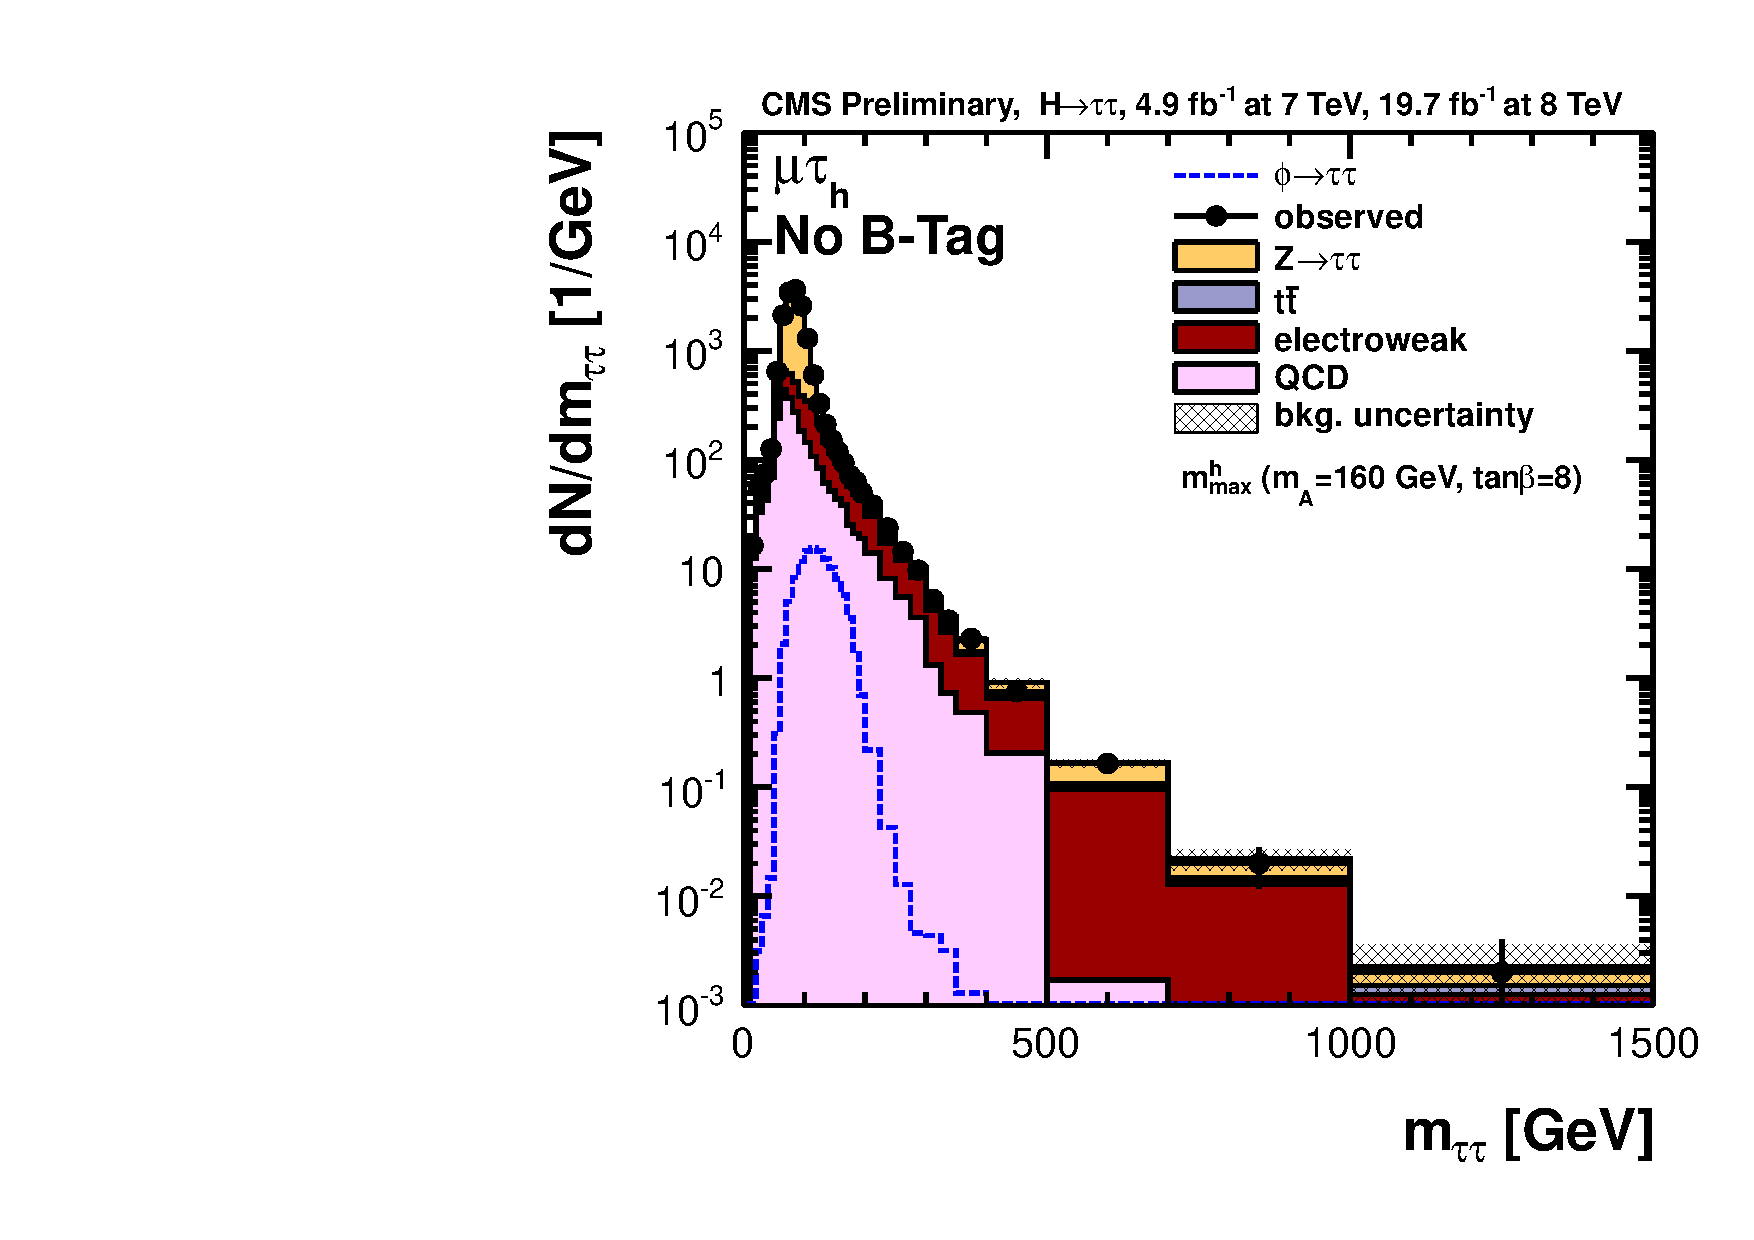
\includegraphics[width=0.45\textwidth]{MSSM/PLOTS/muTau_nobtag_postfit_7+8TeV_LOG.pdf}
 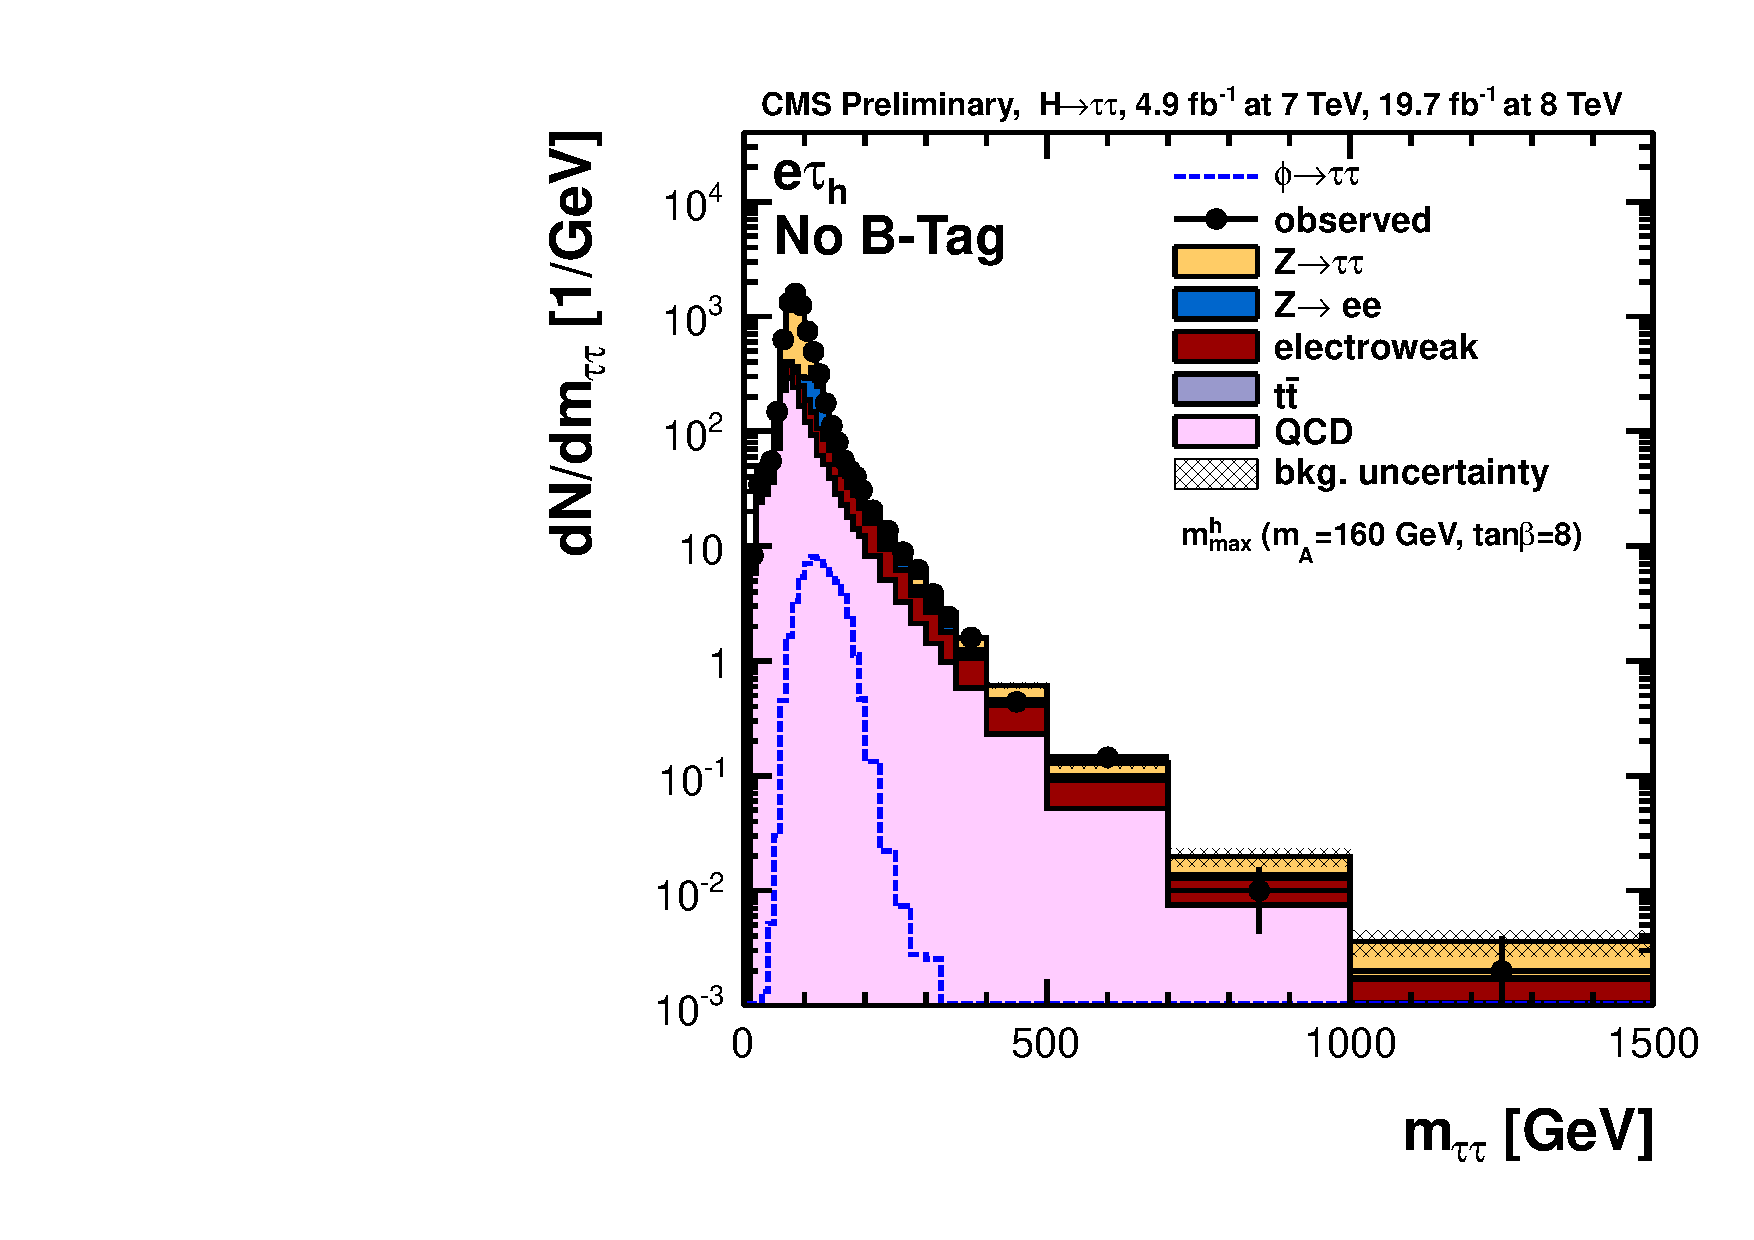
\includegraphics[width=0.45\textwidth]{MSSM/PLOTS/eleTau_nobtag_postfit_7+8TeV_LOG.pdf}
 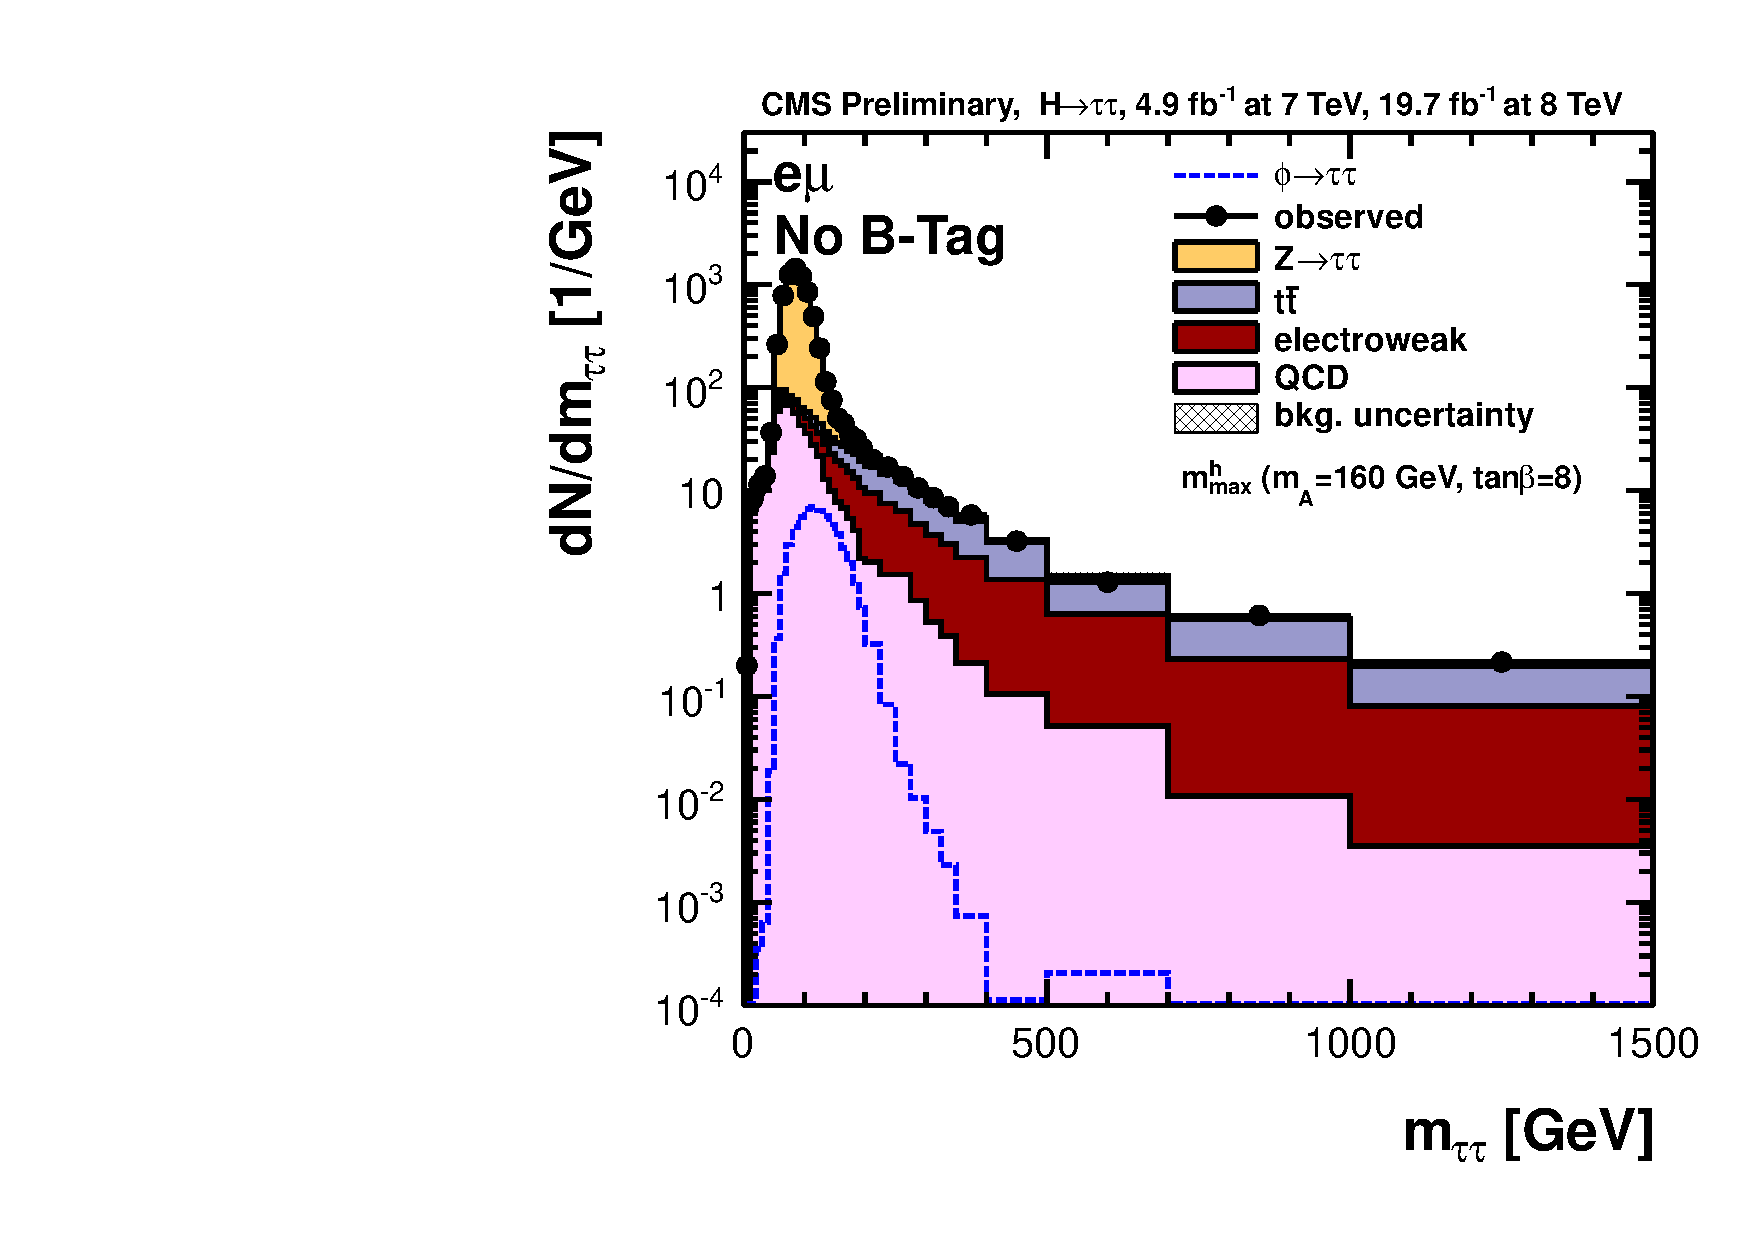
\includegraphics[width=0.45\textwidth]{MSSM/PLOTS/emu_nobtag_postfit_7+8TeV_LOG.pdf}
 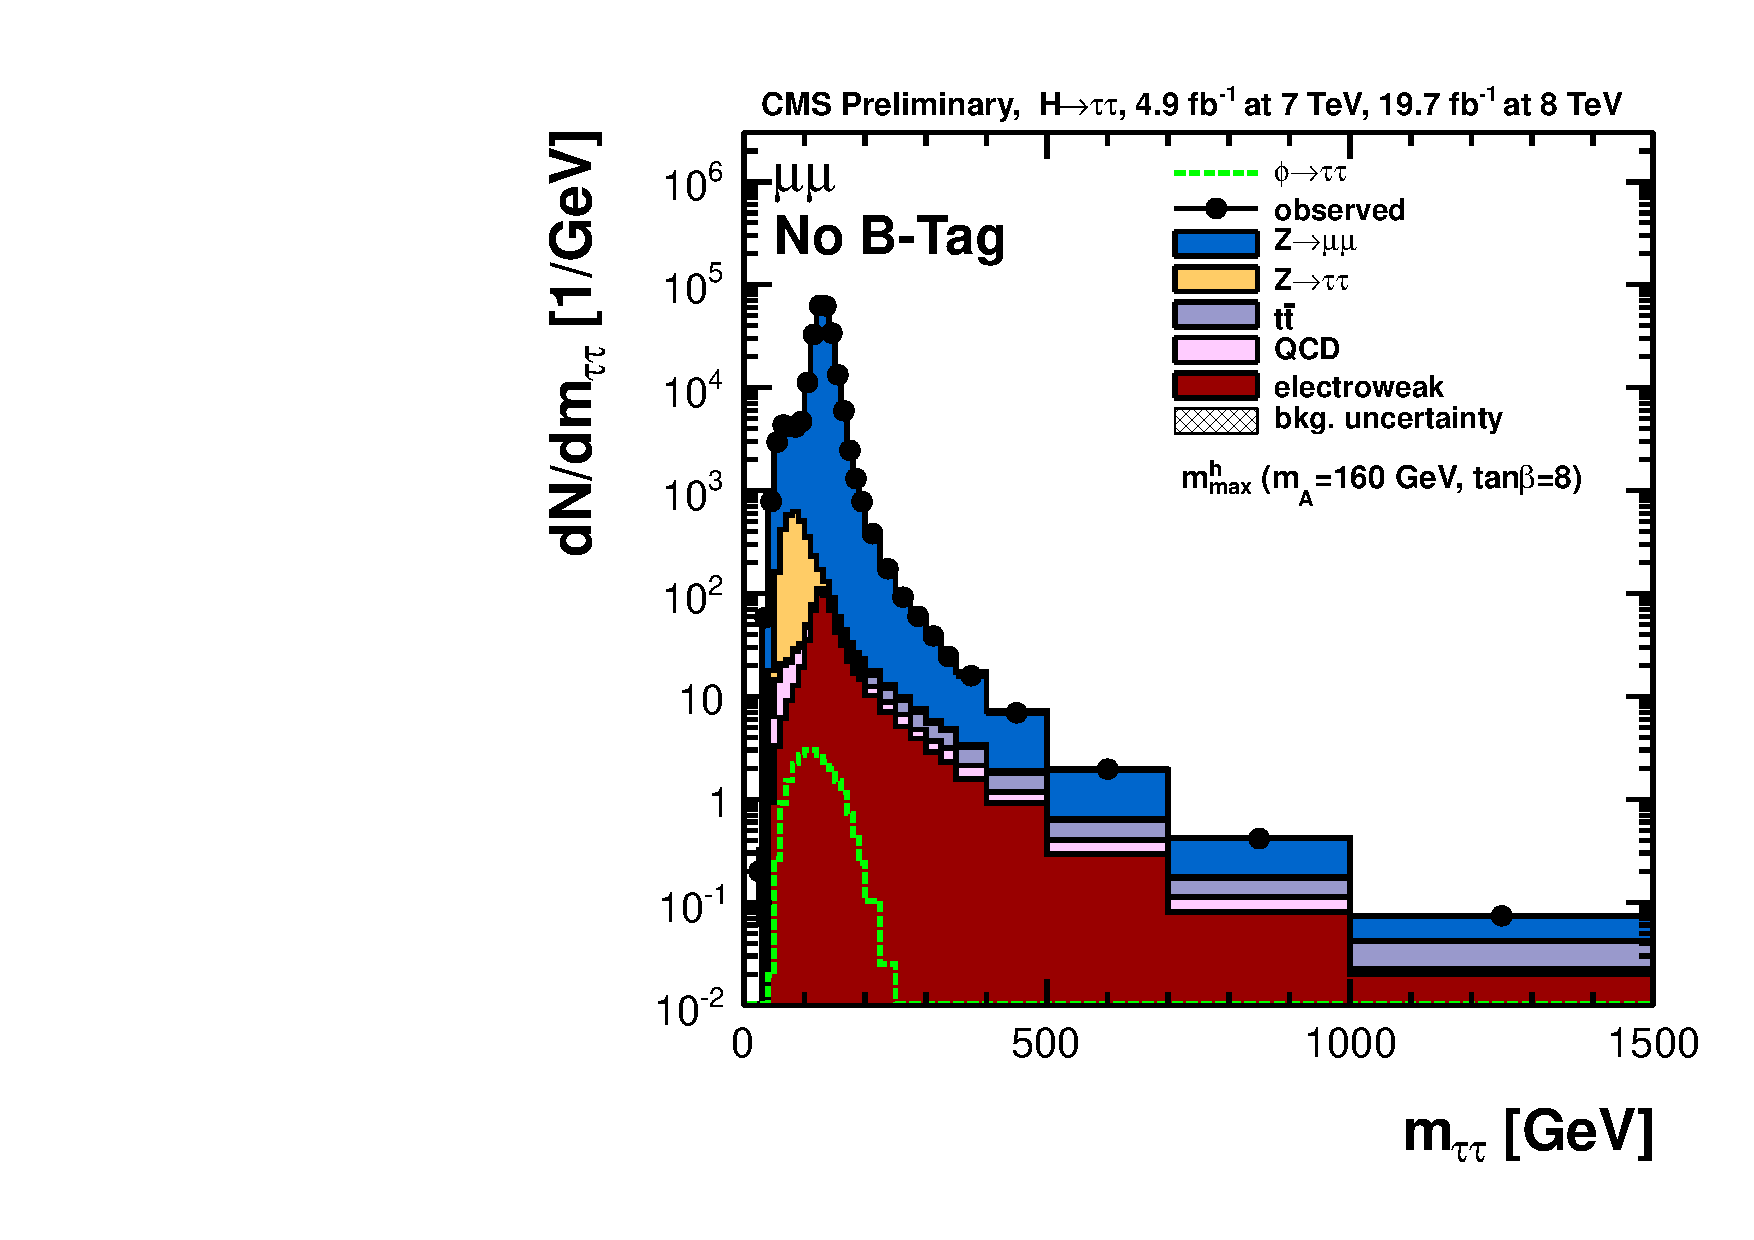
\includegraphics[width=0.45\textwidth]{MSSM/PLOTS/mumu_nobtag_postfit_7+8TeV_LOG.pdf}
 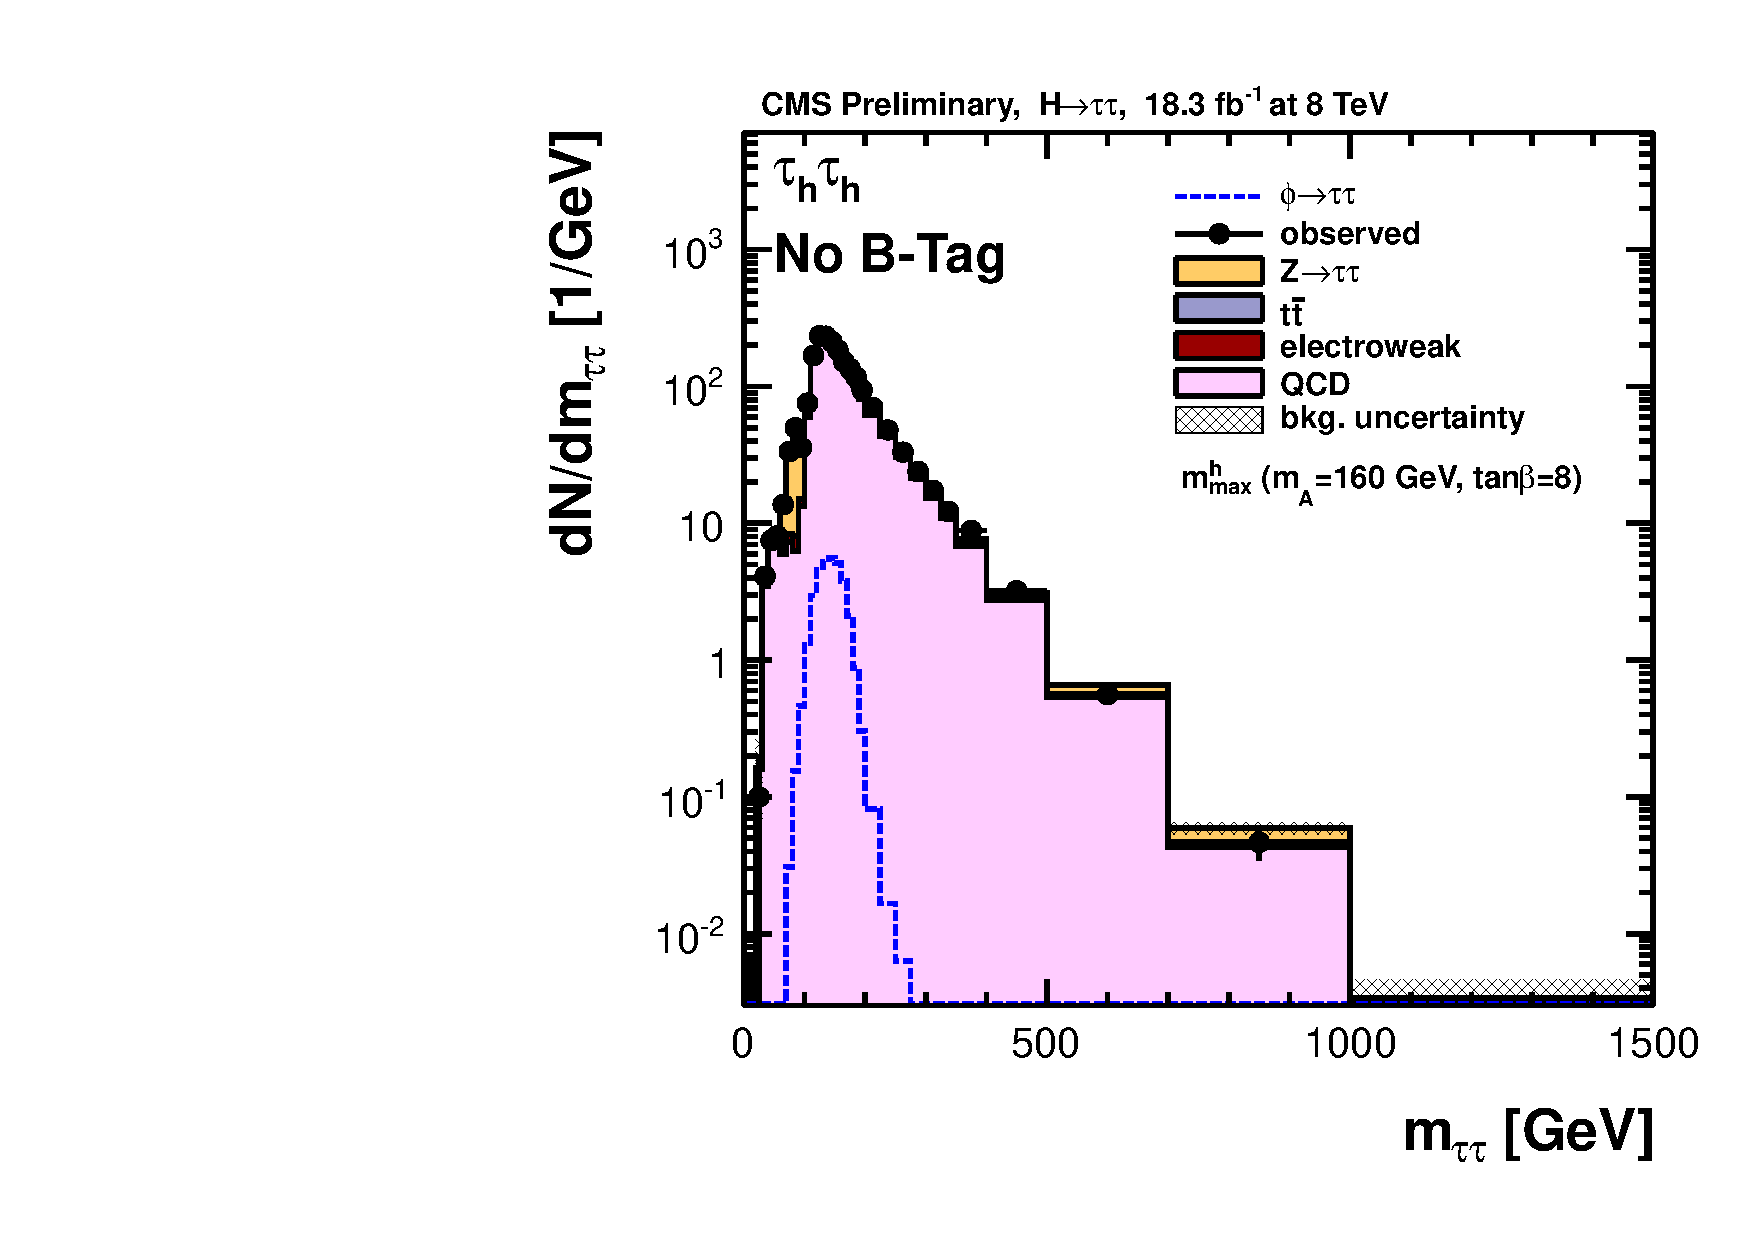
\includegraphics[width=0.45\textwidth]{MSSM/PLOTS/tauTau_nobtag_postfit_8TeV_LOG.pdf}
 \caption{Reconstructed di-$\Pgt$ mass in the no-b-tag category for the $\Pgm\Pgt_{h}, \Pe\Pgt_{h}, \Pe\Pgm$, $\Pgm\Pgm$ and $\Pgt_{h}\Pgt_{h}$ channels.}
  \label{fig:mass_no_b_tag}\end{center}\end{figure*}


\begin{figure*}[!h]\begin{center}
 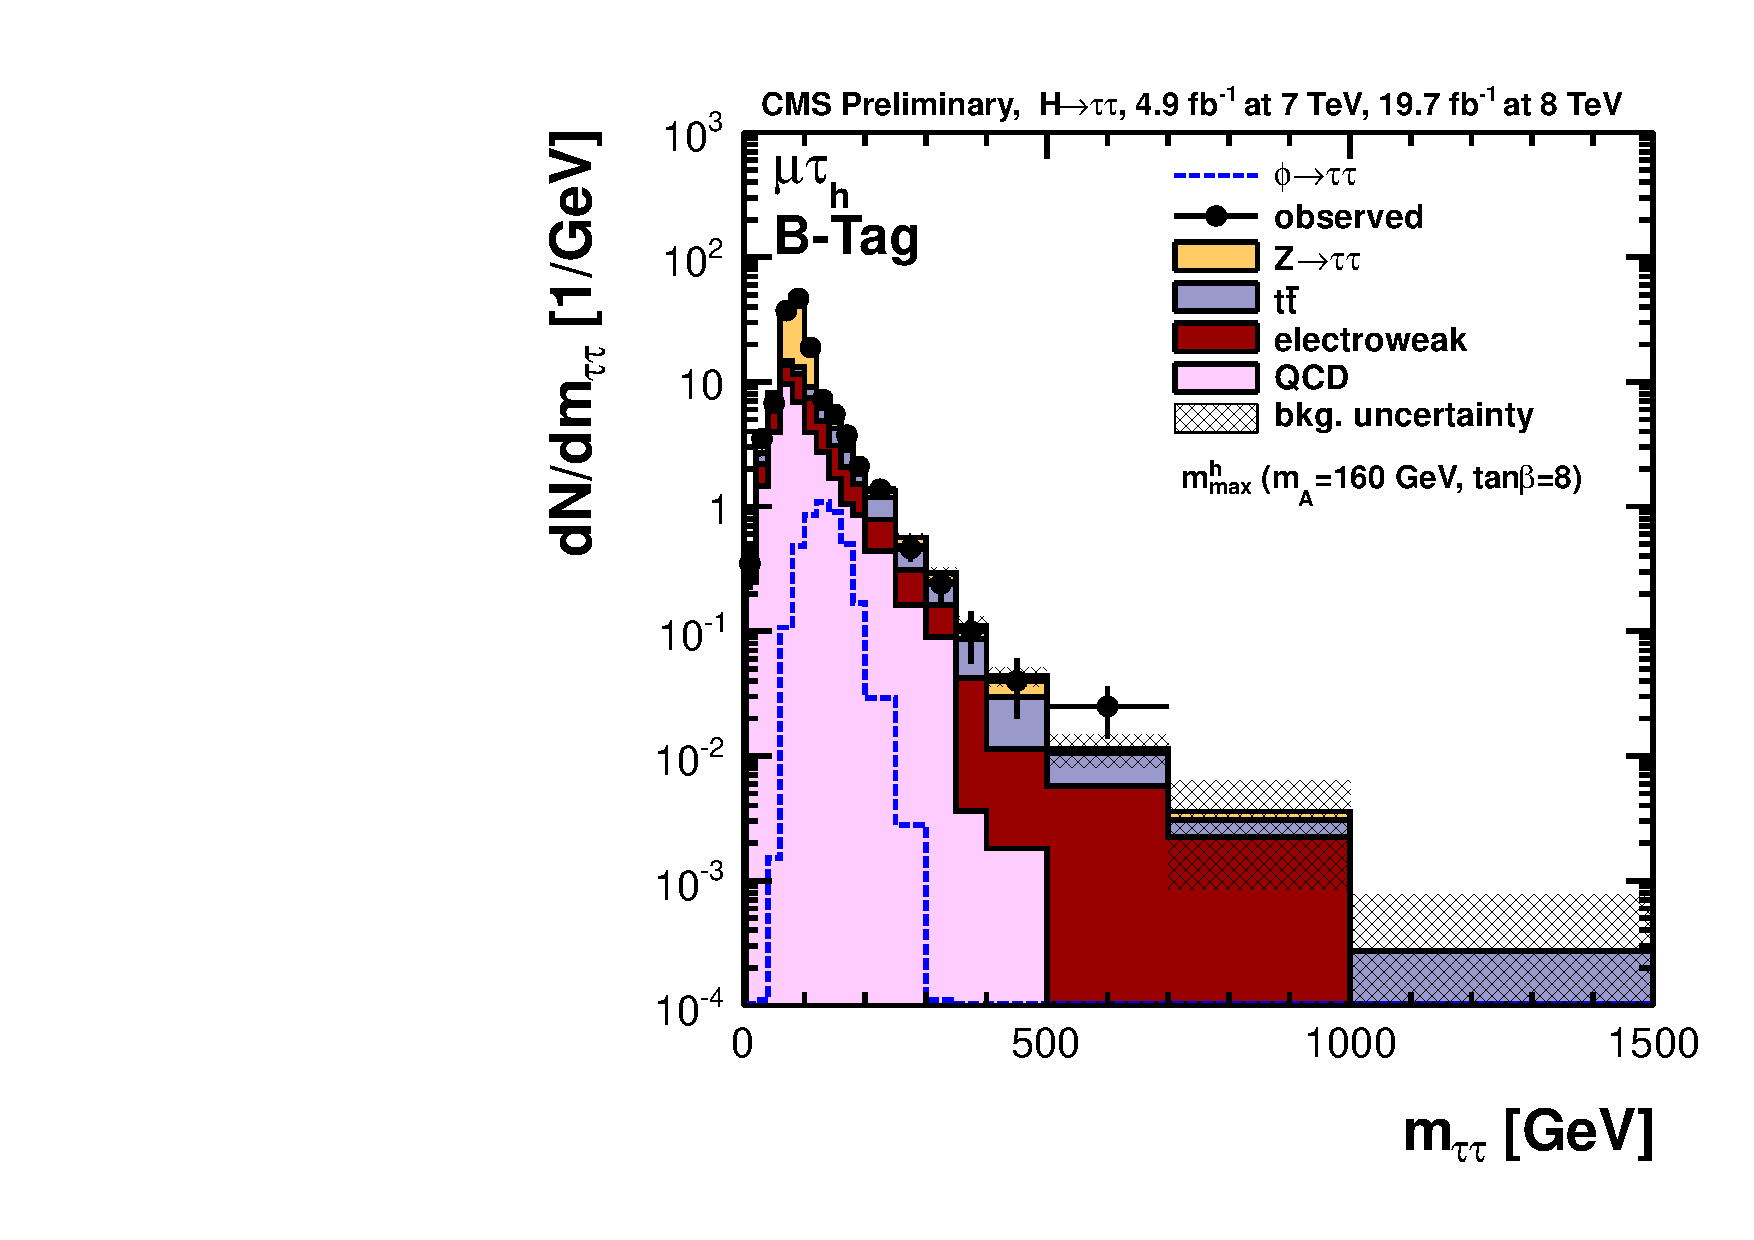
\includegraphics[width=0.45\textwidth]{MSSM/PLOTS/muTau_btag_postfit_7+8TeV_LOG.pdf}
 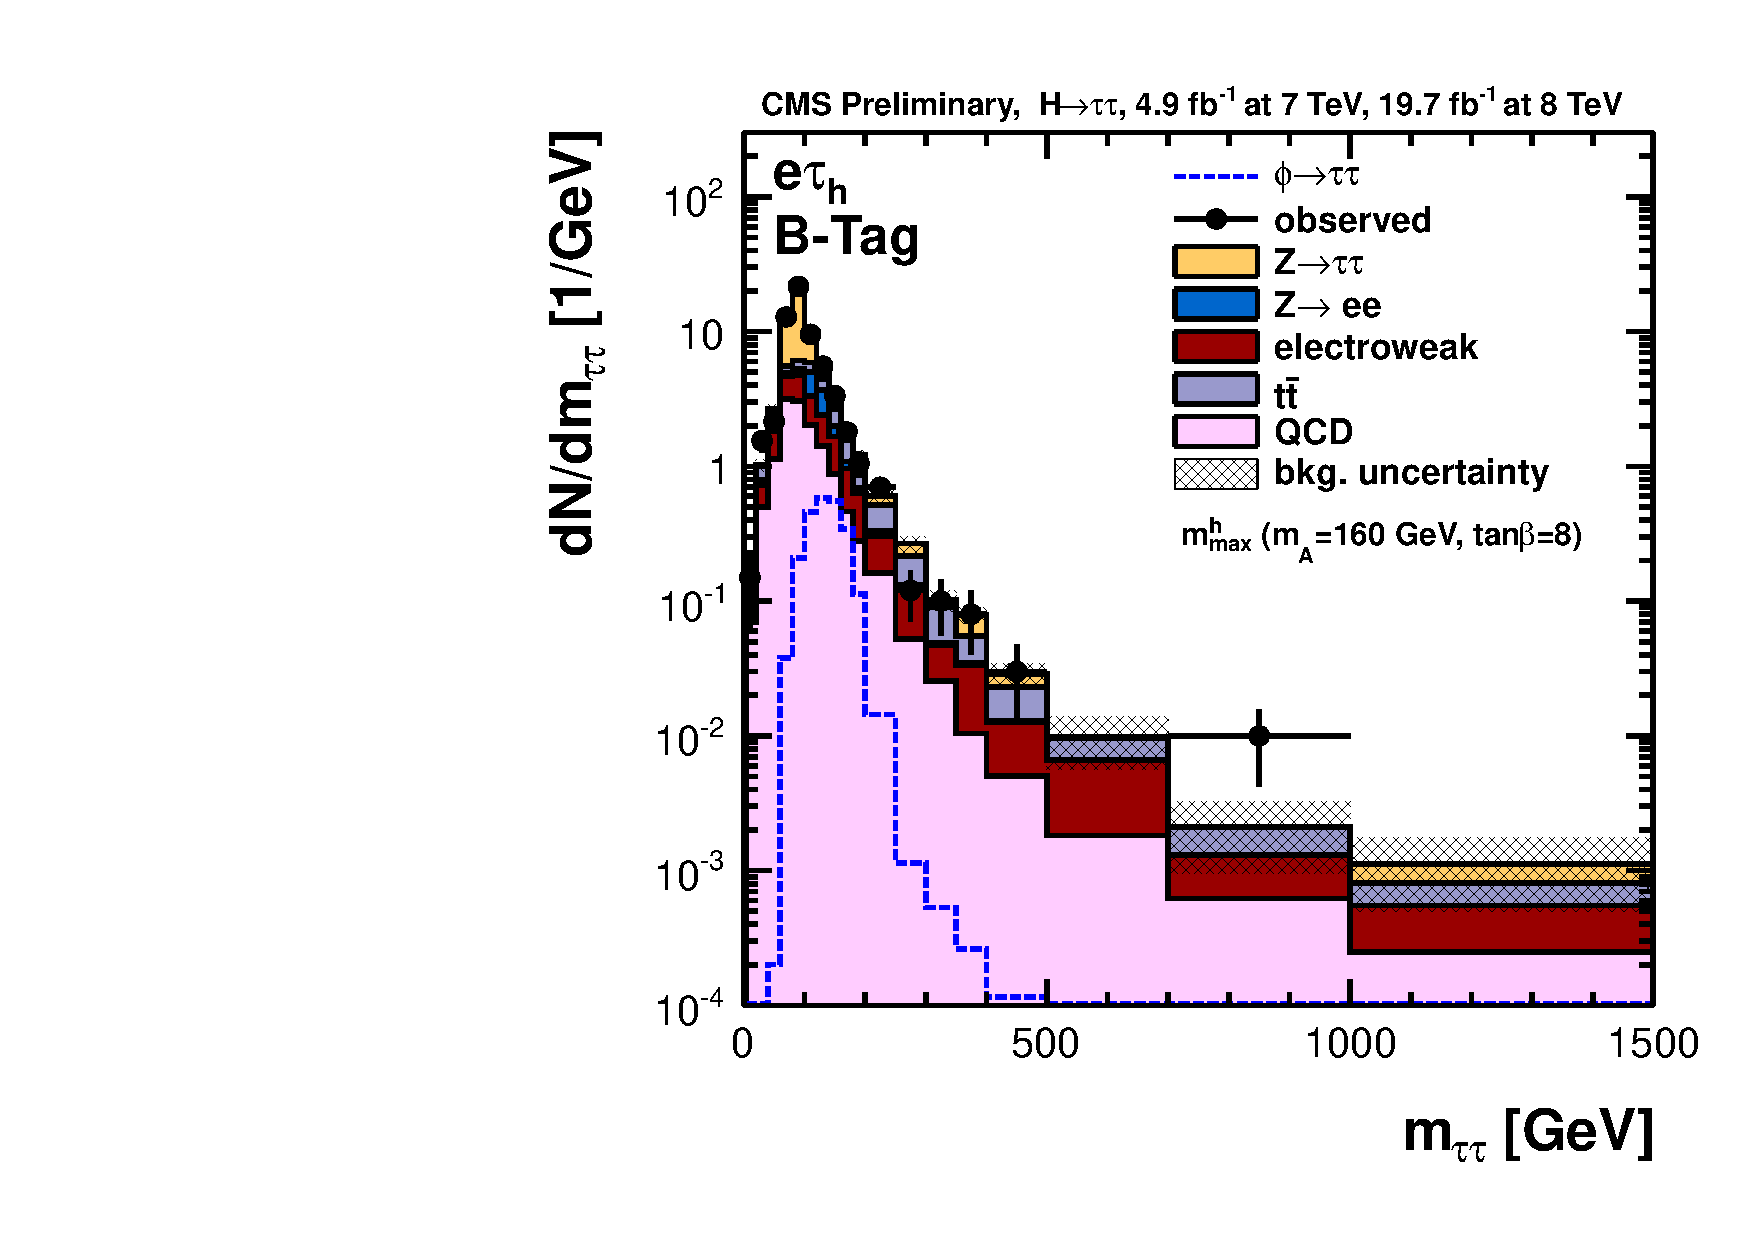
\includegraphics[width=0.45\textwidth]{MSSM/PLOTS/eleTau_btag_postfit_7+8TeV_LOG.pdf}
 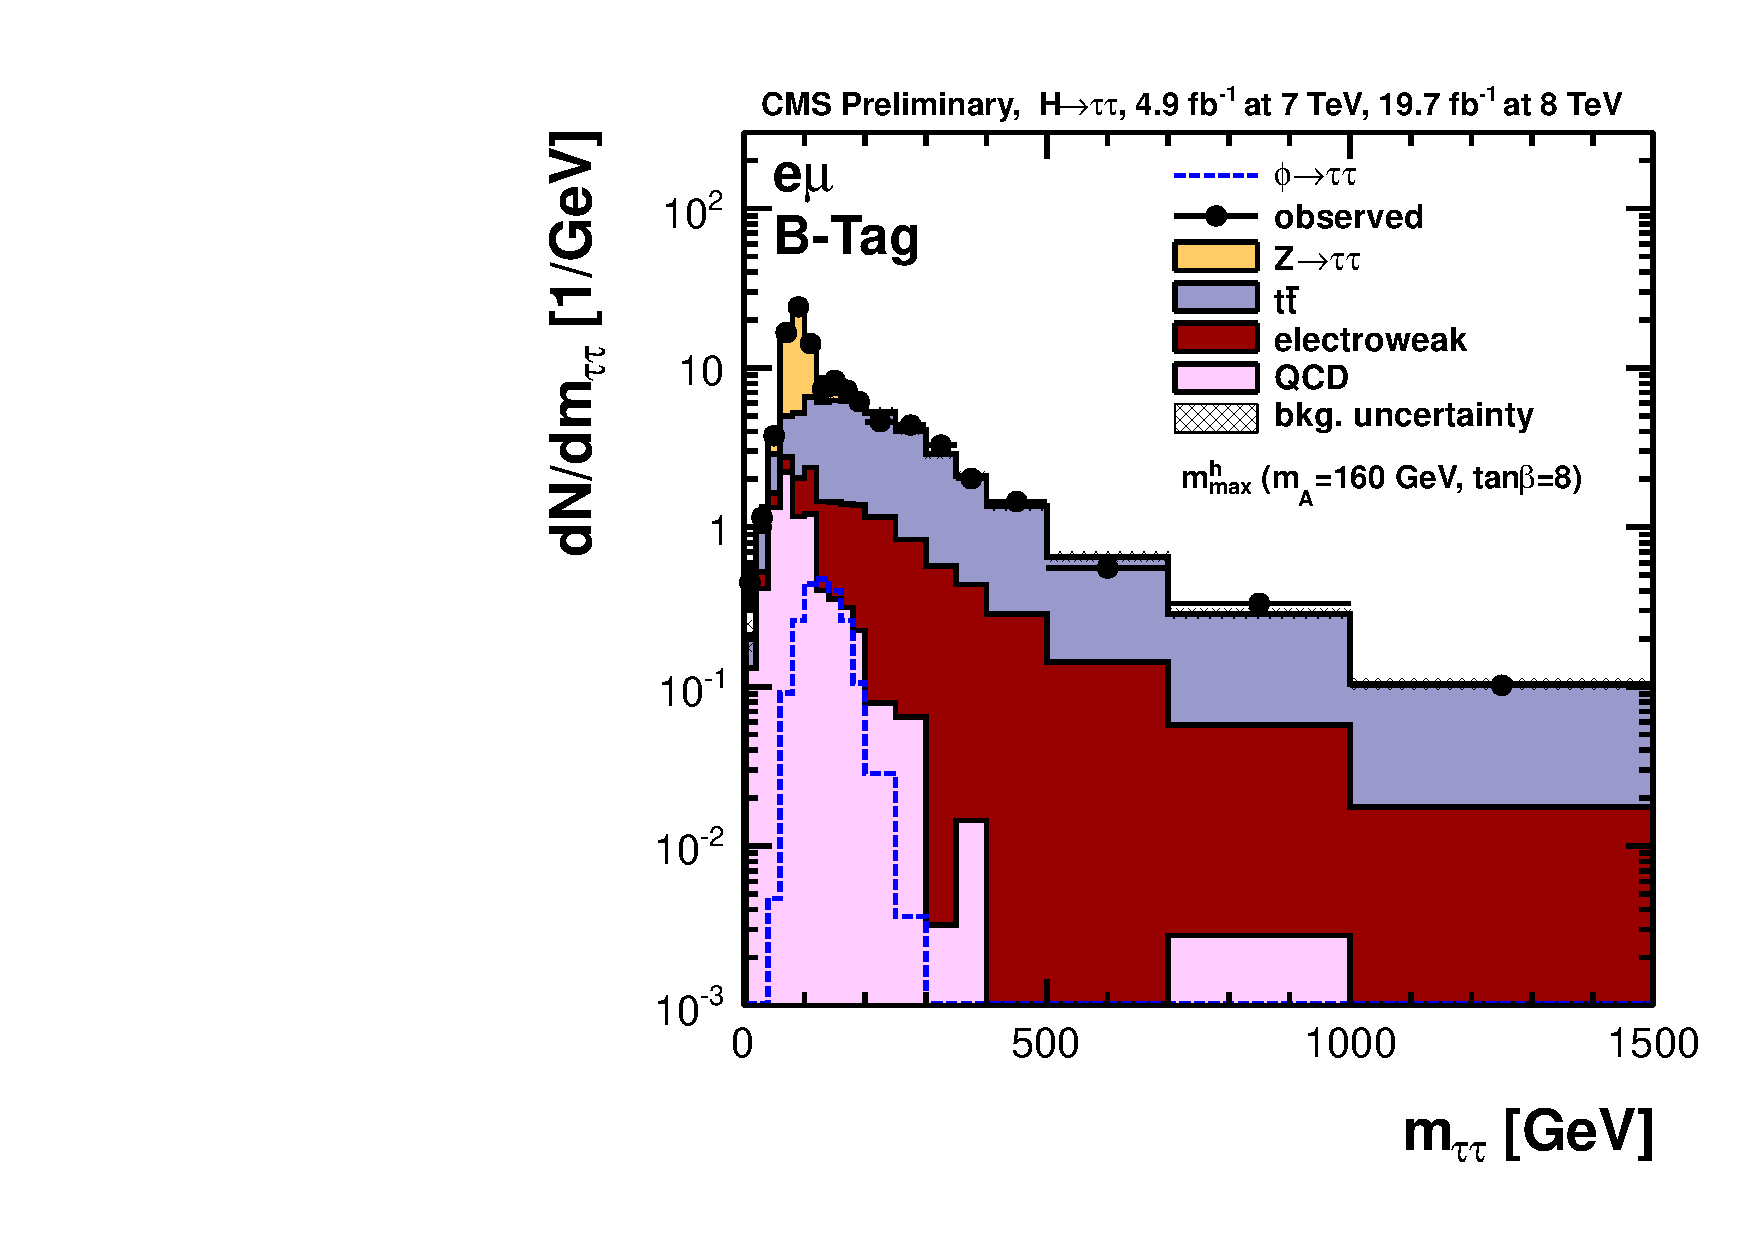
\includegraphics[width=0.45\textwidth]{MSSM/PLOTS/emu_btag_postfit_7+8TeV_LOG.pdf}
 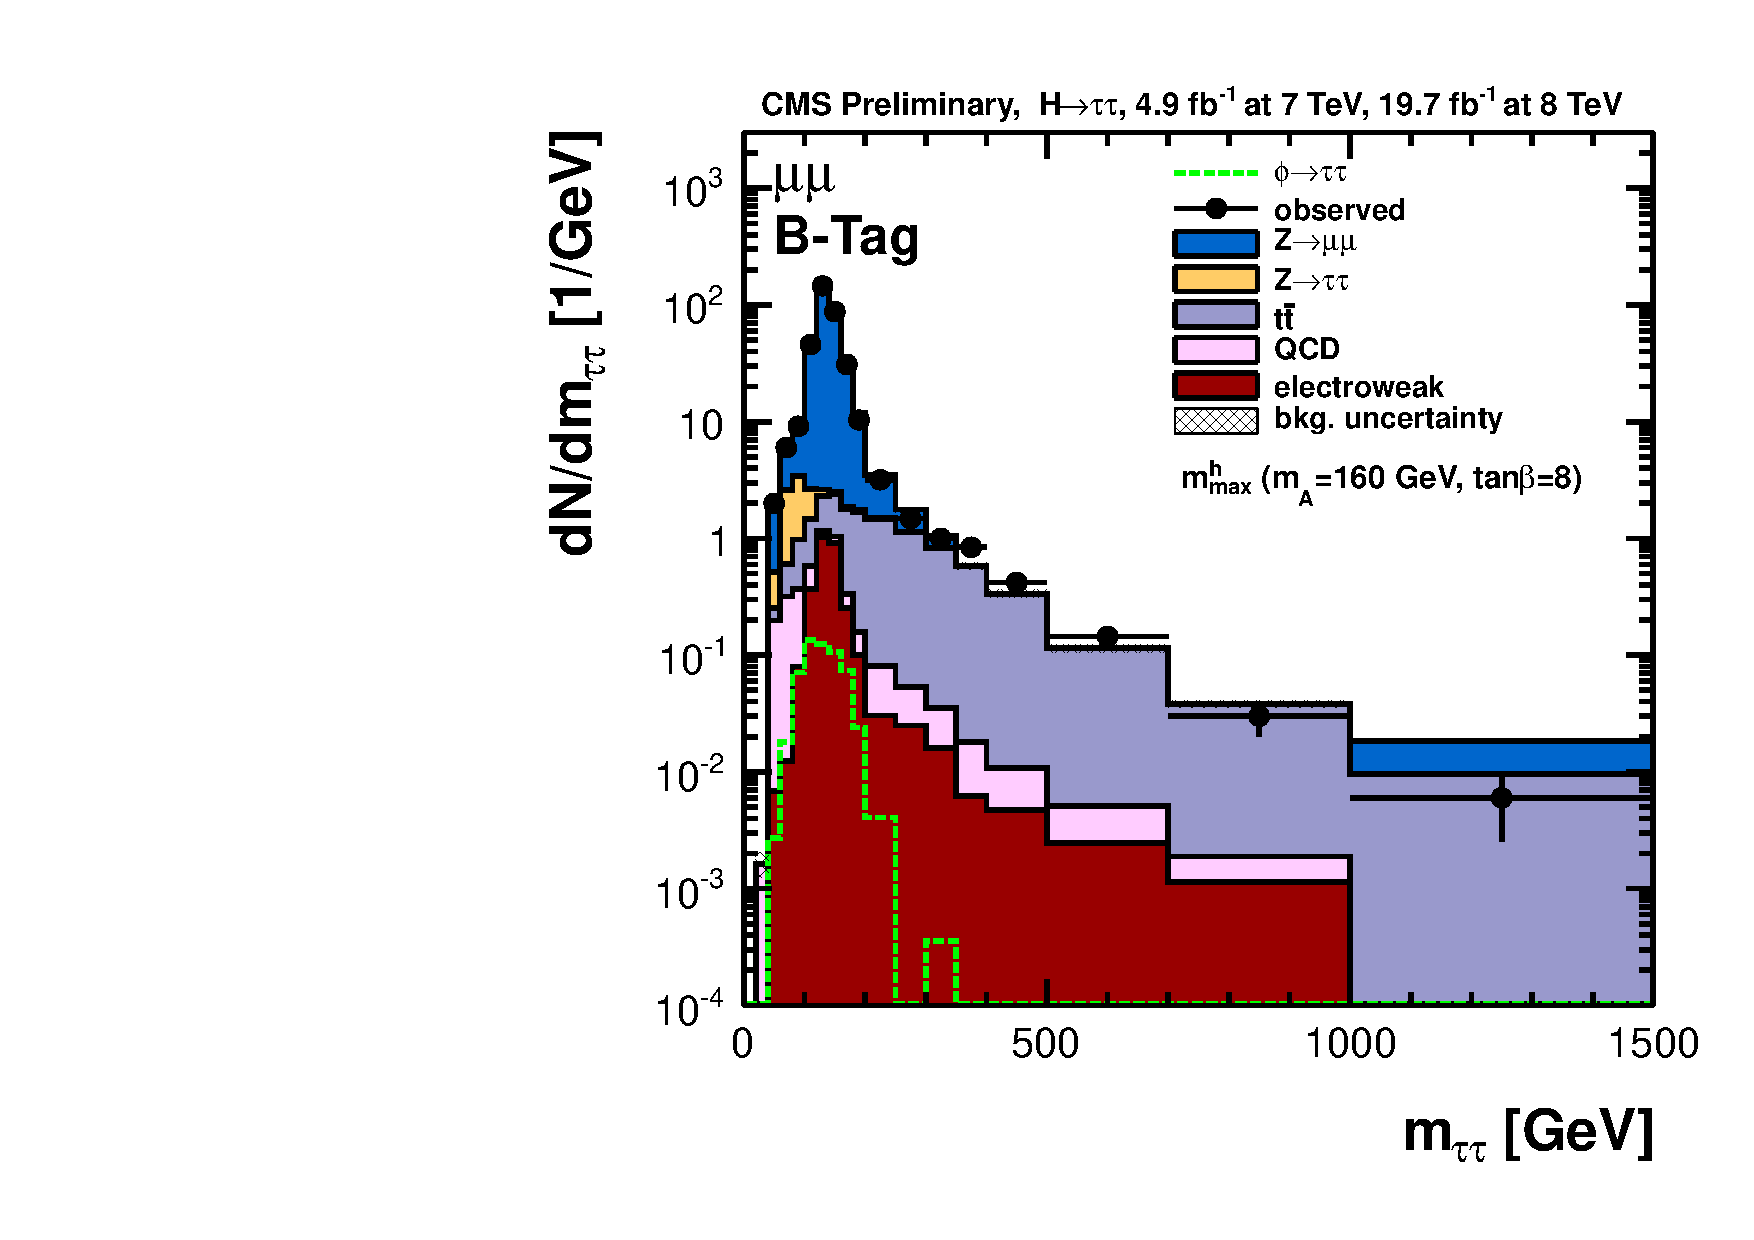
\includegraphics[width=0.45\textwidth]{MSSM/PLOTS/mumu_btag_postfit_7+8TeV_LOG.pdf}
 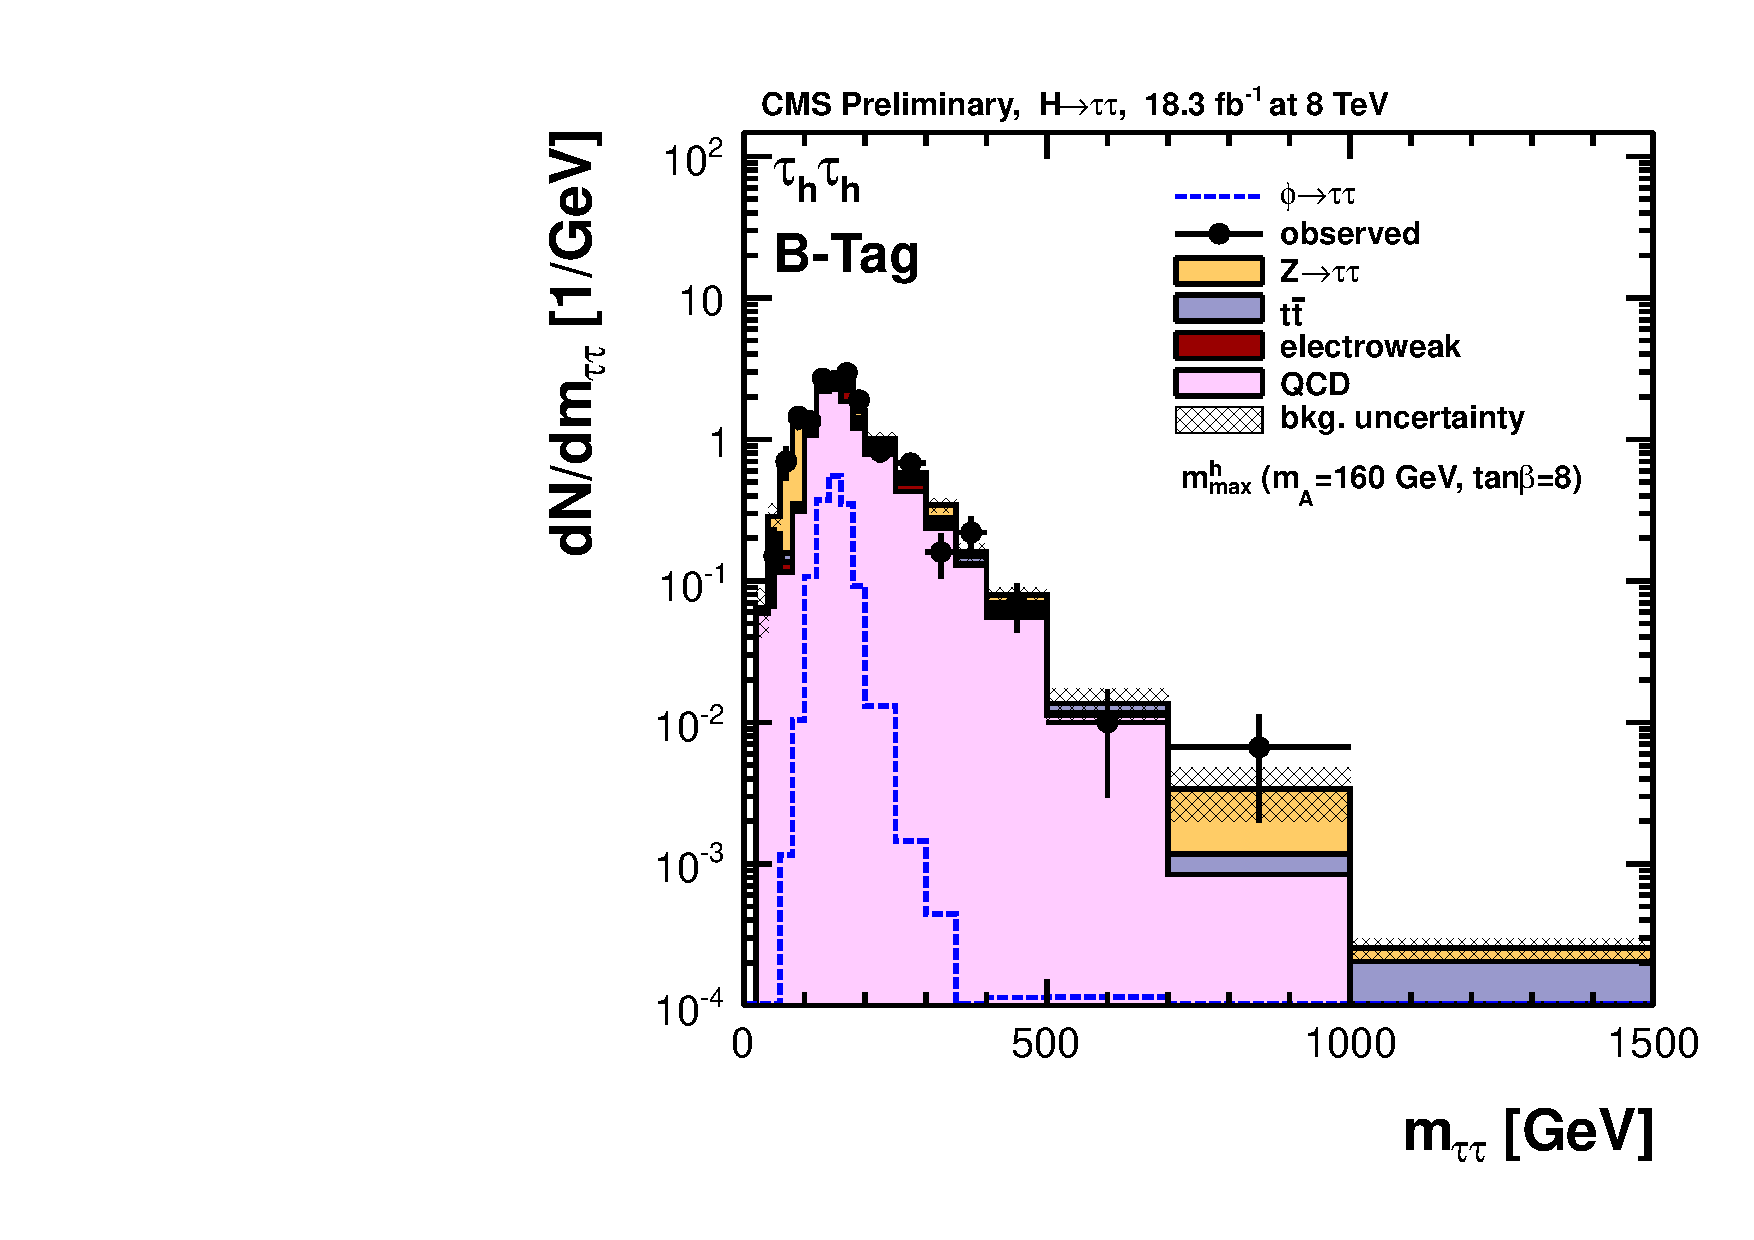
\includegraphics[width=0.45\textwidth]{MSSM/PLOTS/tauTau_btag_postfit_8TeV_LOG.pdf}
 \caption{Reconstructed di-$\Pgt$ mass in the b-tag category for the $\Pgm\Pgt_{h}, \Pe\Pgt_{h}, \Pe\Pgm$, $\Pgm\Pgm$ and $\Pgt_{h}\Pgt_{h}$  channels.}
  \label{fig:mass_b_tag}\end{center}\end{figure*}


The invariant mass spectra show no clear evidence for the presence of a MSSM Higgs boson signal, 
therefore 95\% CL upper bounds on tan$\beta$ as a function of the pseudoscalar Higgs boson mass $M_A$ are set.
The limits are computed using the modified Frequentist method~\cite{Read}.
%Exclusion limits obtained in the tan$\beta$ and $M_A$ plane for the $m_{h}^{\rm max}$ MSSM benchmark scenario are shown in Tab.~\ref{tab-limits}. 

%Signal contributions from $h$, $H$ and $A$ production are considered in the limit setting procedure.
%The limit is computed by performing a scan in the tan$\beta$ and $M_A$ plane.
%At each scan point, the signal expectation for the sum of $h$, $H$ and $A$ is computed as described before.
%The relative contributions of gluon fusion and b-associated production are computed for the tan$\beta$ value under consideration.
%A point in the tan$\beta$ and $M_A$ plane is excluded by the data
%if the ratio of signal-plus-background to background-only hypothesis, $CL_{s} = \{frac{P_{S+B}}{1 - P_{B}}}$, is below $5\%$.

%In the fit, signal contributions from $h$, $H$ and A production are considered. The relative contributions of gluon fusion and b-associated production are taken for different tan$\beta$ values for each mass hypothesis.  The $m_{h}^{\rm max}$ scenario is used, and yields conservative expected limits in the tan$\beta$ and $M_A$ plane. 
%In this scenario, the parameters are set to the following values: $M_{\rm SUSY}$ = 1~TeV; $X_t$ =2$M_{\rm SUSY}$; $\Pgm$ =~200~$\GeV$; $M_{\tilde{g}}$ = 800~$\GeV$; $M_2$ = 200~$\GeV$; and $A_b = A_t$, where $M_{\rm SUSY}$ is the common soft-SUSY-breaking squark mass of the third generation; $X_t = A_t - \Pgm/\tan\beta$ is the stop mixing parameter; $A_t$ and $A_b$ are the stop and sbottom trilinear couplings, respectively; $\Pgm$ the Higgsino mass parameter; $M_{\tilde{g}}$ the gluino mass; and $M_2$ is the SU(2)-gaugino mass parameter. The value of $M_1$ is fixed via the unification relation $M_1 =(5/3)M_2\sin\theta_{\rm W}/\cos\theta_{\rm W}$.



\clearpage


%Fig.~\ref{fig:tanbeta_ma} shows the 95\% CL exclusion in the tan$\beta$-$M_{A}$ parameter space for the MSSM m$_{\rm h}^{\rm max}$ scenario. 
%The expected limit has been computed for the case that no, i.e. neither a MSSM nor a SM, Higgs signal is present in the data.
%The limit expected in case a Standard Model Higgs boson is present in the data is shown separately in the figure.
%The presence of a SM Higgs boson is expected to make a difference of 1-2 units in tan$\beta$ at low $M_{A}$.
%At high $M_{A}$ the presence of a SM Higgs boson is seen to still have some effect on the expected limit;
%this is because a SM Higgs boson would appear as a signal peak compatible with the light scalar MSSM Higgs $h$.
%The exclusion limits set by the LEP experiments are also shown.
%Numerical values for the expected and observed exclusion limits are given in Tab.~\ref{tab-limits}. 

Figure~\ref{fig:tanbeta_ma} shows the 95\% CL exclusion in the tan$\beta$-$M_{A}$ parameter space for the MSSM m$_{\rm h}^{\rm max}$ scenario. 
The exclusion limit set by the LEP experiments~\cite{LEP2-MSSM} is also shown.
Numerical values for the expected and observed exclusion limits are given in Tab.~\ref{tab-limits}. 
The expected limit has been computed for the case that no Higgs signal, neither of SM nor of MSSM type, is present in the data.
The limit expected in case a SM Higgs boson is present in the data is computed separately 
and differs by 1-2 units in tan$\beta$ at low $M_{A}$.
At high $M_{A}$ there is also some effect as the limit is mainly
driven by the light scalar Higgs $h$, which has the largest expected cross section.

\begin{figure}[!h]
\setlength{\unitlength}{1mm}
\begin{center}
\begin{picture}(150,90)(0,0)
\put(-10.5, -2.0){\mbox{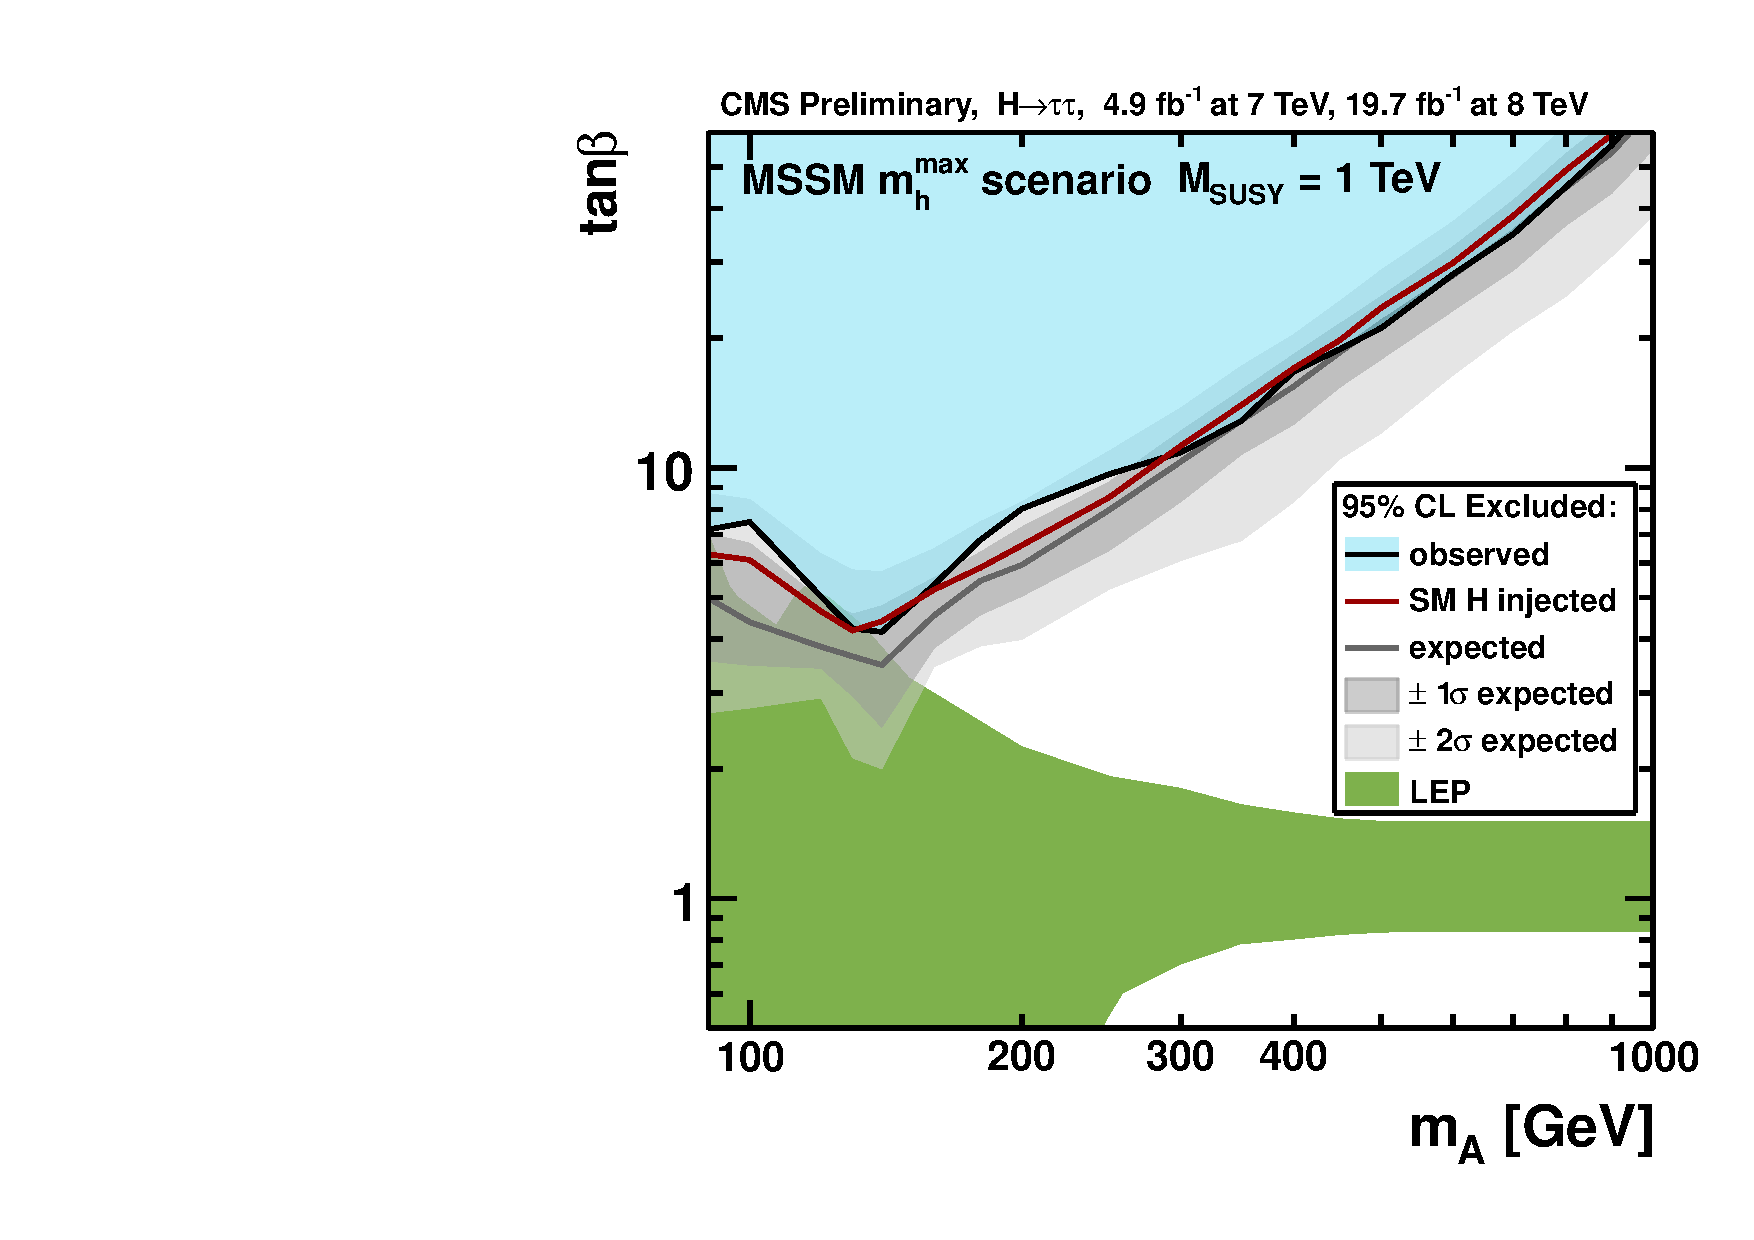
\includegraphics[width=96mm]{MSSM/PLOTS/limit_tanBeta_vs_mA_log.pdf}}}
\put(86.0, 8.0){\mbox{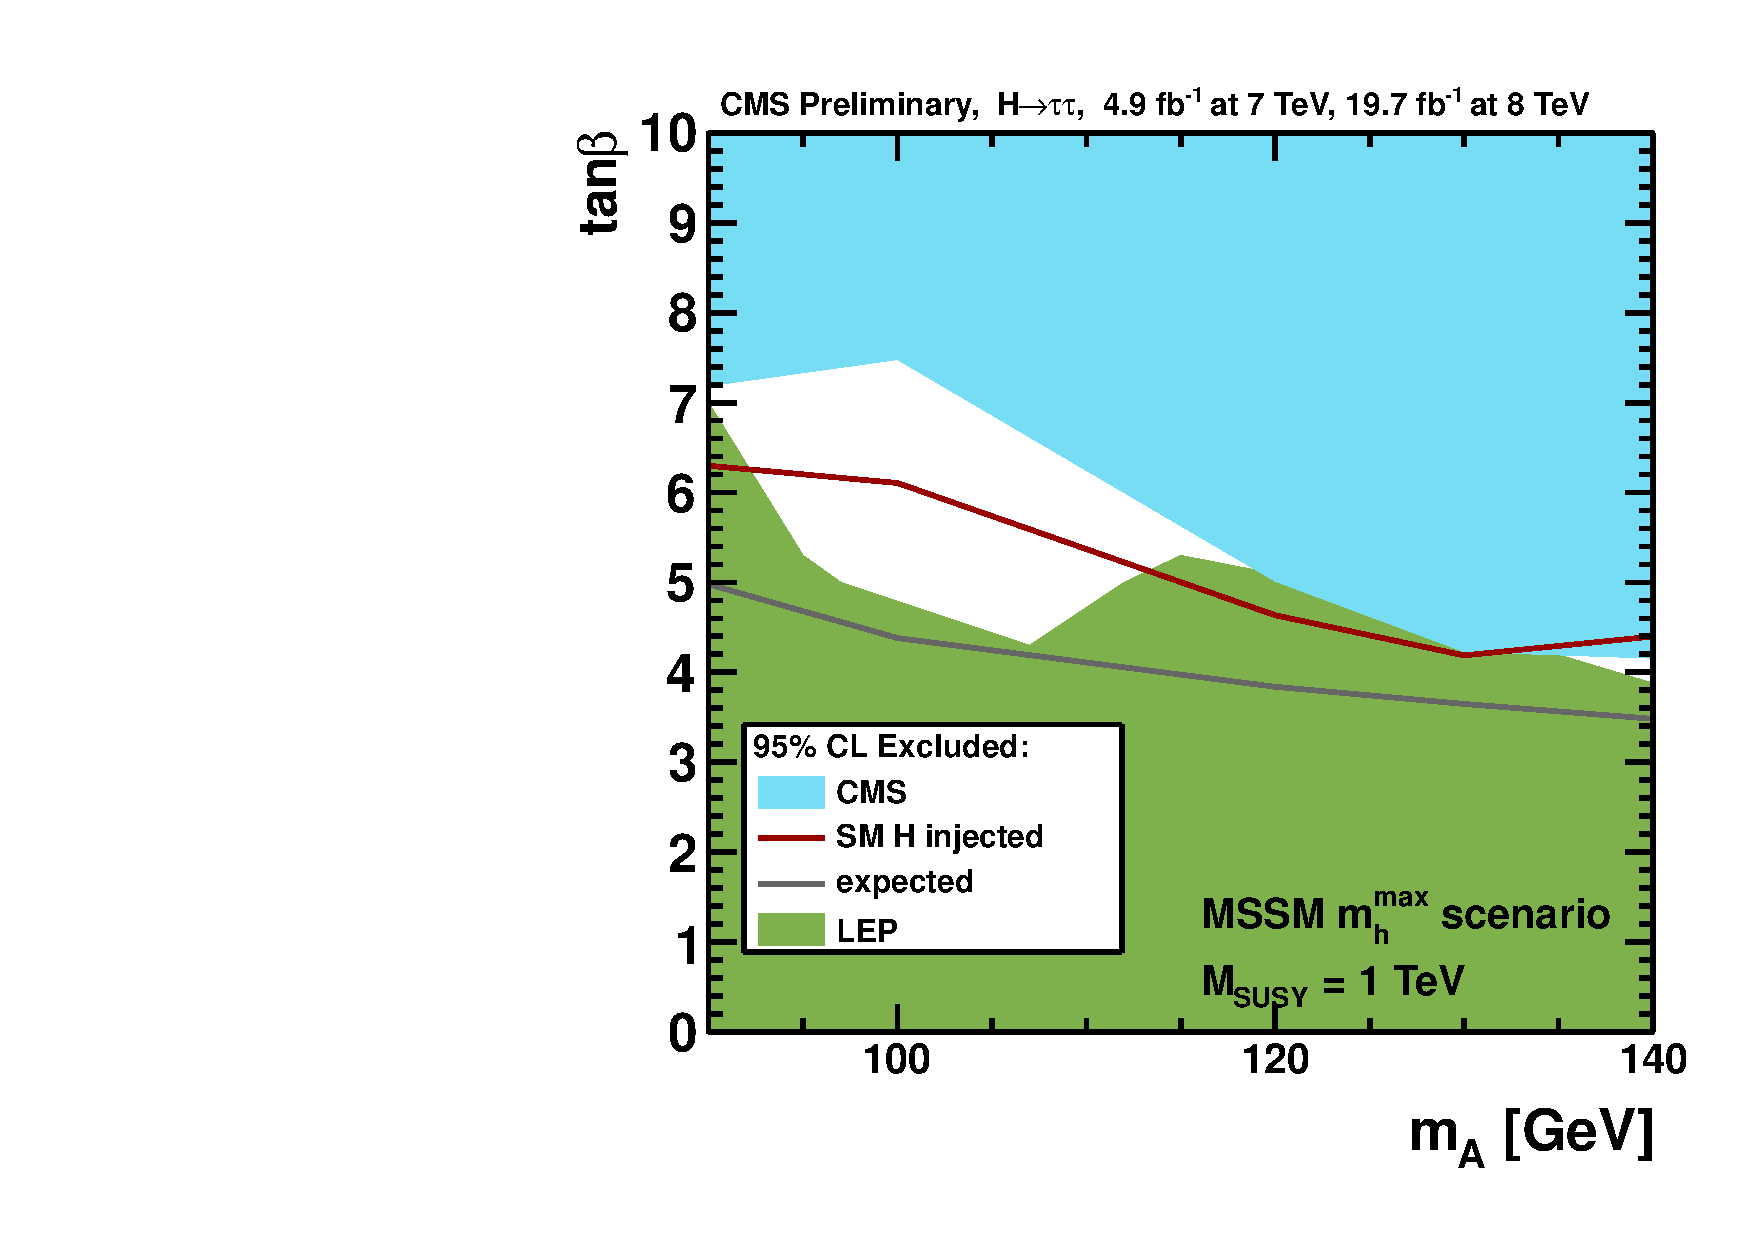
\includegraphics[width=72mm]{MSSM/PLOTS/limit_tanBeta_vs_mA_linear_ZOOM.pdf}}}
\end{picture}
%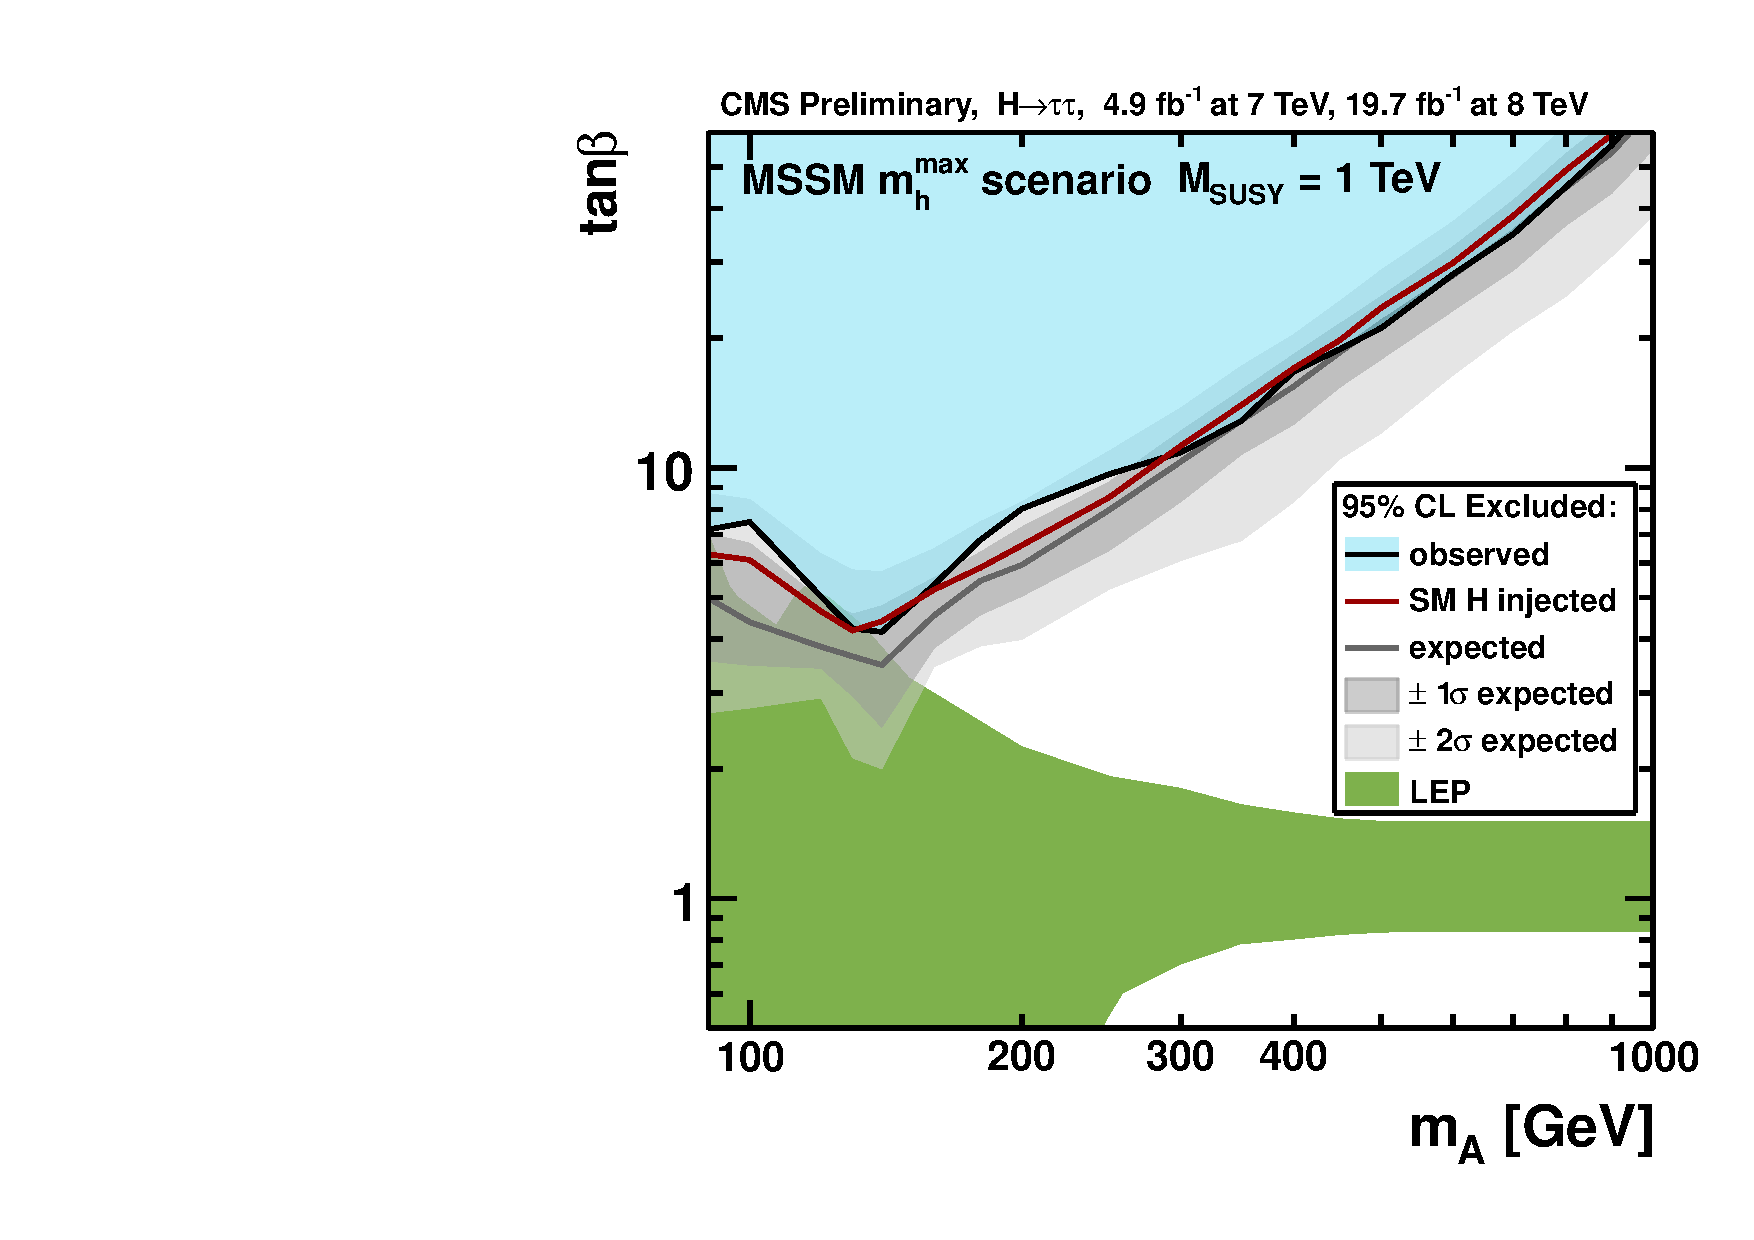
\includegraphics[width=110mm]{MSSM/PLOTS/limit_tanBeta_vs_mA_log.pdf}
%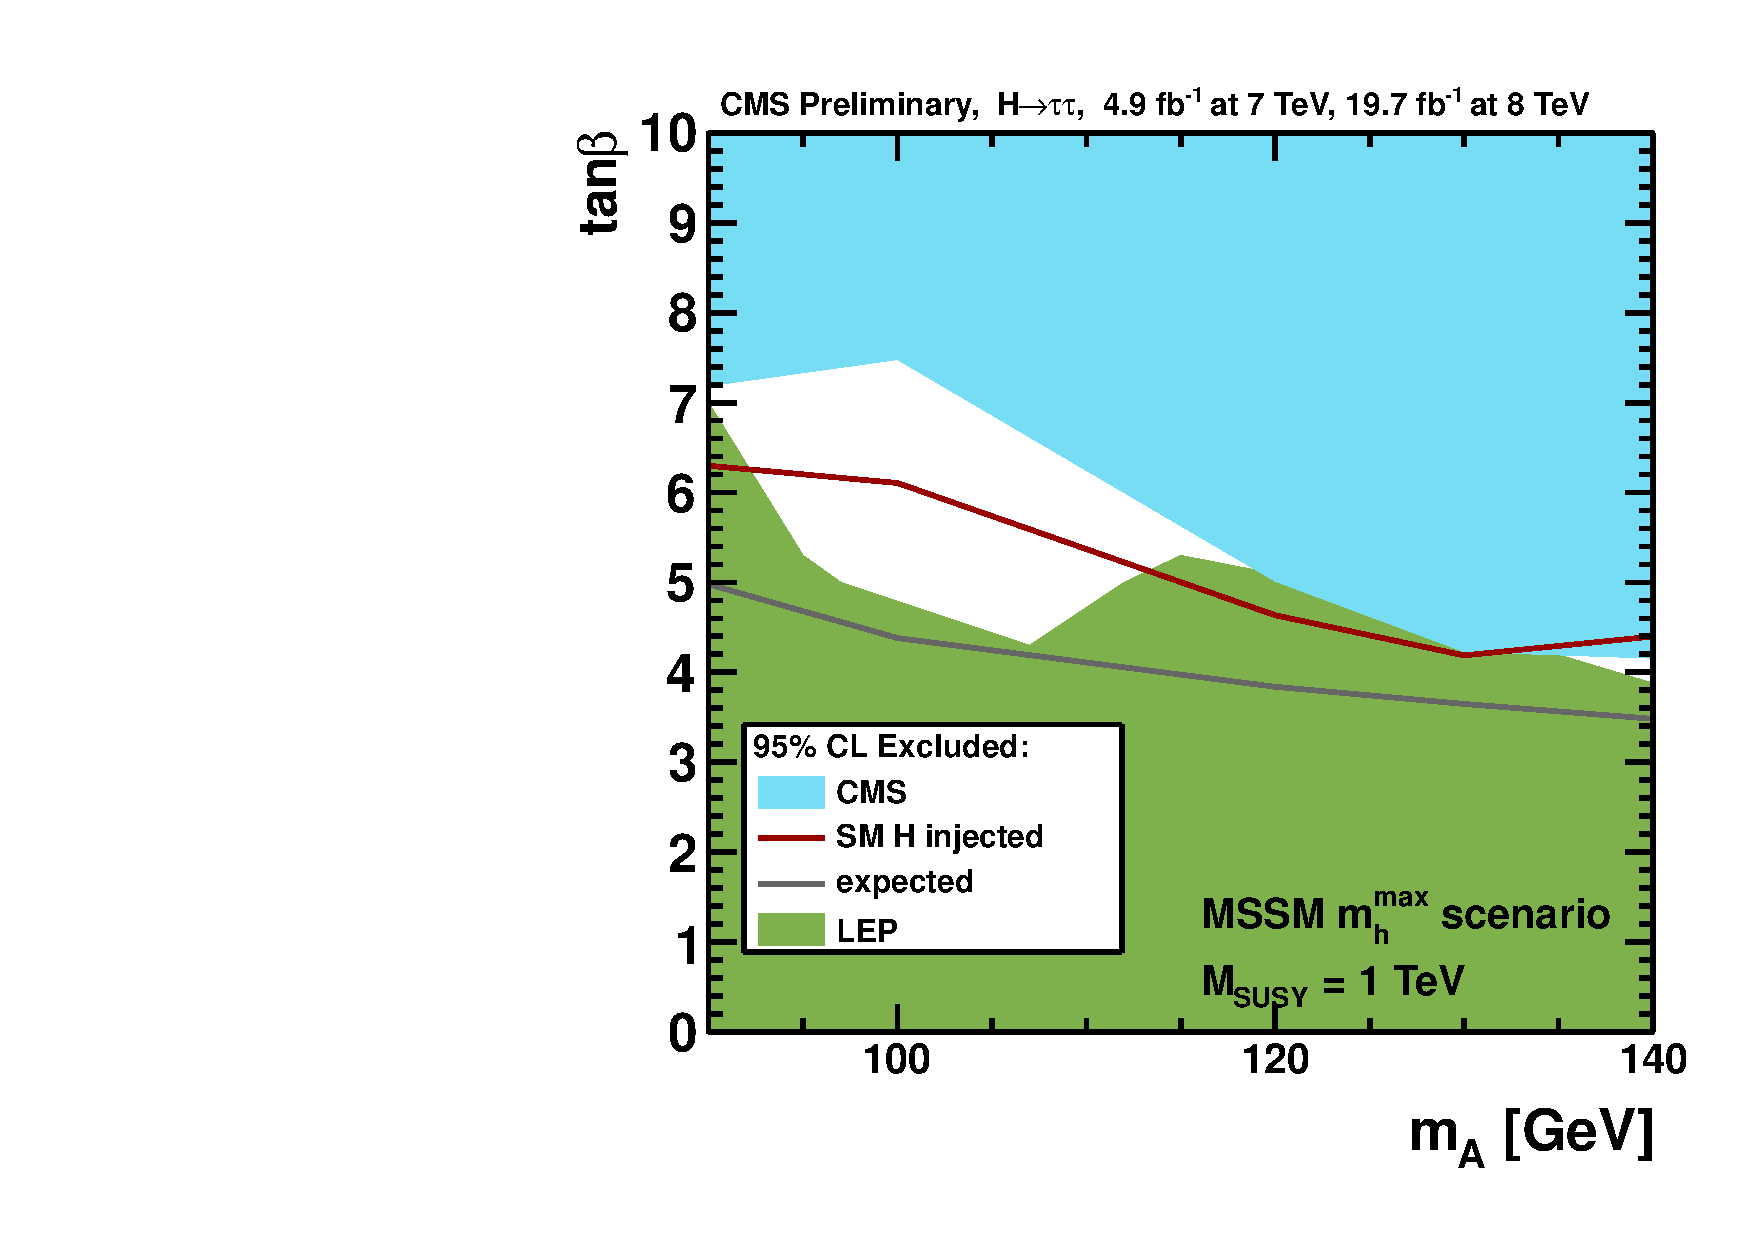
\includegraphics[width=110mm]{MSSM/PLOTS/limit_tanBeta_vs_mA_linear_ZOOM.pdf}
\end{center}
\caption{
  Left: Exclusion at 95\% CL in the tan$\beta$-$M_{A}$ parameter space for the MSSM m$_{\rm h}^{\rm max}$ scenario. The exclusion limits from the LEP experiments are also shown.
  Expected limits are computed for two cases:
  for the assumption that there is no Higgs $\to \tau\tau$ signal
  (neither MSSM nor SM) present in the data (dark grey line)
  and assuming that there is no MSSM, but a SM Higgs of mass
  $125$--$126$~$\GeV$ present (red line).
  Right: 95\% CL exclusion limit in the low $M_{A}$ region. 
  %The uncertainty bands around the expected limit are omitted to see more clearly the region in parameter space not excluded by CMS or LEP data (white area).
}
\label{fig:tanbeta_ma}
\end{figure}


\begin{table*}[!h]
  \begin{center}
    \caption{Expected range and observed 95\% CL upper limits for
             $\tan\beta$ as a function of $M_A$, for the MSSM search.
}
%%{\small
\begin{tabular}{|c|c|c|c|c|c|c|}
\cline{2-7}
\multicolumn{1}{c}{MSSM Higgs}      & \multicolumn{5}{|c|}{Expected $\tan\beta$ limit}   &  Observed \\
\cline{1-6}
  $m_\mathrm{A}$ [GeV] &$-2\sigma$  &   $-1\sigma$ &        Median &    $+1\sigma$ &  $+2\sigma$ & $\tan\beta$ limit \\ 
\hline
                90~$\GeV$ &            2.70 &            3.56 &            4.98 &            7.02 &            8.71 &            7.19  \\
\hline
               100~$\GeV$ &            2.77 &            3.48 &            4.38 &            6.68 &            8.44 &            7.48  \\
\hline
               120~$\GeV$ &            2.92 &            3.42 &            3.84 &            4.94 &            6.30 &            5.01  \\
\hline
               130~$\GeV$ &            2.12 &            2.95 &            3.65 &            4.57 &            5.79 &            4.23  \\
\hline
               140~$\GeV$ &            2.00 &            2.50 &            3.48 &            4.78 &            5.74 &            4.16  \\
\hline
               160~$\GeV$ &            3.45 &            3.81 &            4.54 &            5.56 &            6.49 &            5.35  \\
\hline
               180~$\GeV$ &            3.86 &            4.55 &            5.46 &            6.36 &            7.49 &            6.80  \\
\hline
               200~$\GeV$ &            3.99 &            5.03 &            5.95 &            7.28 &            8.32 &            8.02  \\
\hline
               250~$\GeV$ &            5.22 &            6.43 &            7.98 &            9.27 &           10.9 &            9.66  \\
\hline
               300~$\GeV$ &            6.09 &            8.34 &           10.3 &           12.2 &           13.8 &           10.9  \\
\hline
               350~$\GeV$ &            6.77 &           10.7 &           12.9 &           15.1 &           17.2 &           12.8  \\
\hline
               400~$\GeV$ &            8.33 &           12.6 &           15.4 &           18.3 &           20.4 &           16.7  \\
\hline
               450~$\GeV$ &           10.5 &           15.4 &           18.5 &           21.6 &           24.4 &           18.8  \\
\hline
               500~$\GeV$ &           12.0 &           17.9 &           21.7 &           25.0 &           28.8 &           21.1  \\
\hline
               600~$\GeV$ &           16.4 &           23.1 &           27.9 &           32.6 &           37.2 &           28.1  \\
\hline
               700~$\GeV$ &           20.8 &           28.7 &           35.2 &           41.8 &           48.2 &           34.9  \\
\hline
               800~$\GeV$ &           25.0 &           36.5 &           44.7 &           53.6 &           $> 60$$^{1}$ &           44.8  \\
\hline
               900~$\GeV$ &           31.0 &           43.4 &           53.9 &           $> 60$\,$^{1}$ &          $> 60$\,$^{1}$ &           $> 60$\,$^{1}$  \\
\hline
              1000~$\GeV$ &           38.5 &           54.9 &          $> 60$\,$^{1}$ &           $> 60$\,$^{1}$ &          $> 60$\,$^{1}$ &           $> 60$\,$^{1}$  \\
\hline
 \end{tabular}
%%} % end small
    \label{tab-limits}
  \end{center}
$^{1}$ We do not quote limits above $\tan\beta = 60$ as the theoretical calculations
which provide the relation between cross section and $\tan\beta$ 
become unreliable at high $\tan\beta$. 
\end{table*}

\clearpage

Model independent limits on $\sigma\cdot$BR($\Phi\to\Pgt\Pgt$) for gluon-fusion and b-associated Higgs production as a function of the Higgs mass
have been determined.
The results for 8 TeV center-of-mass energy are shown in Fig.~\ref{fig:ggH_bbH_limit}.
In this case, a single resonance search (for a resonance of mass $m_{\Phi}$) is performed.  The results are also shown in Tables~\ref{ggH-limit} and~\ref{bbH-limit}.
Figures~\ref{fig:contour1}-~\ref{fig:contour4} show the 2-dimensional 68\% and 95\% CL likelihood scans of $\sigma\cdot$BR($\Phi\to\Pgt\Pgt$) for gluon-fusion and b-associated Higgs production, for different Higgs masses.



\begin{figure*}[!h]\begin{center}
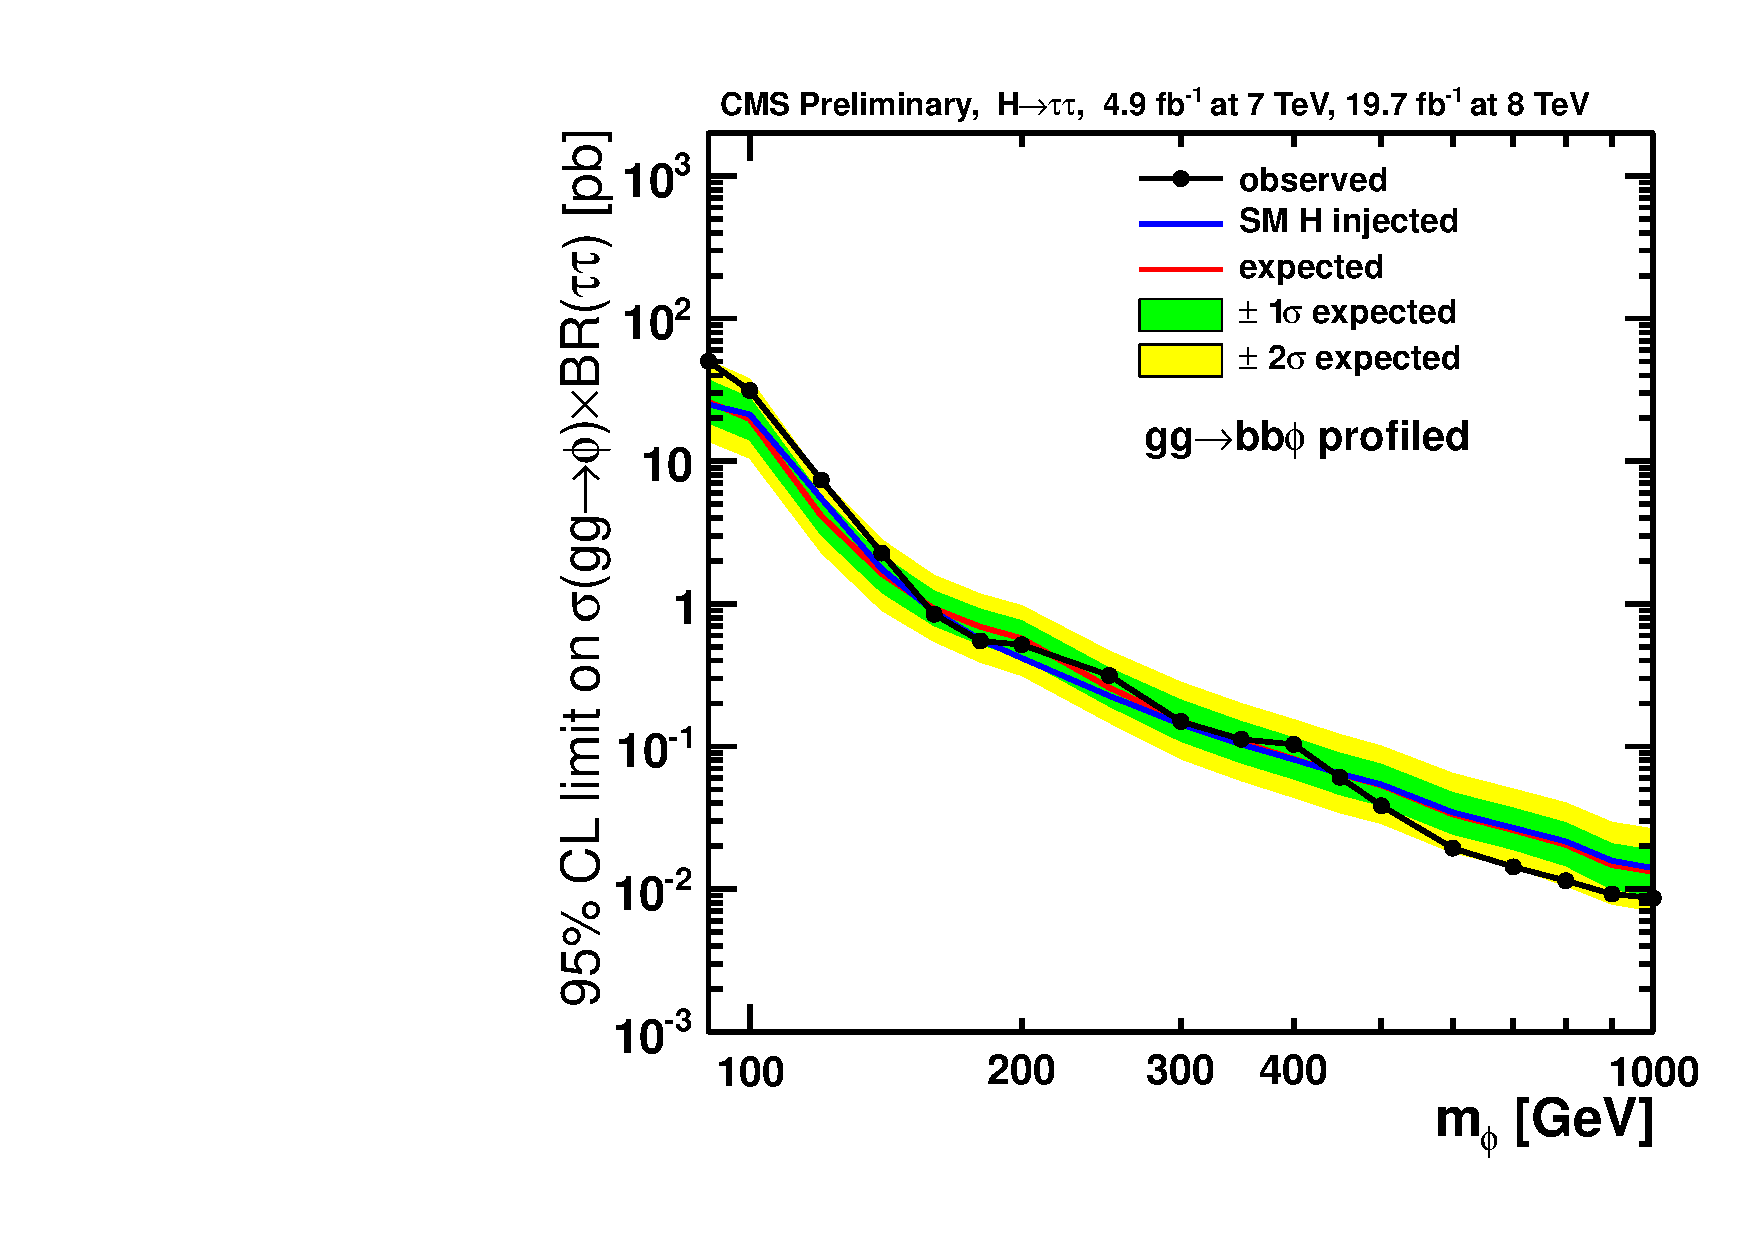
\includegraphics[width=0.45\textwidth]{MSSM/PLOTS/cmb_ggH-limit.pdf}
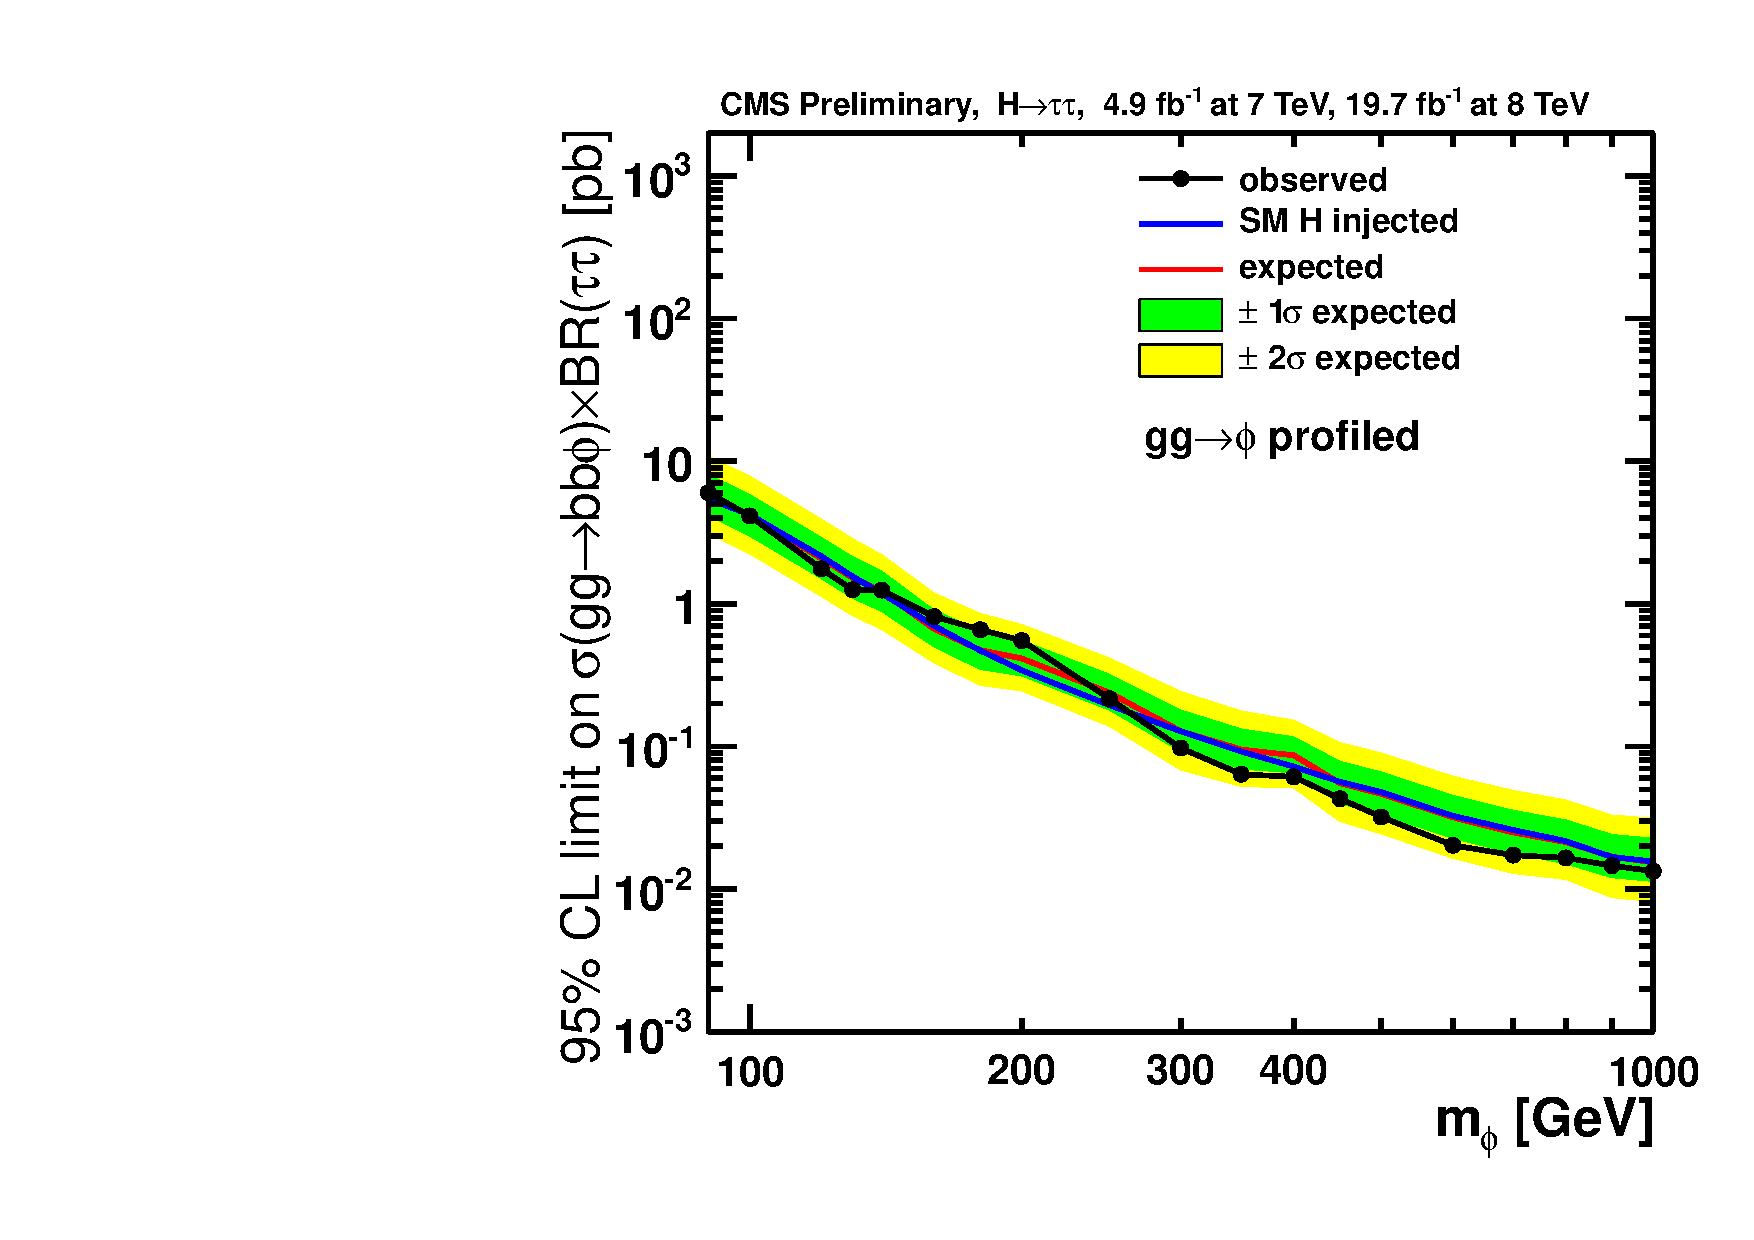
\includegraphics[width=0.45\textwidth]{MSSM/PLOTS/cmb_bbH-limit.pdf}
\caption{
  95\% CL upper limit on $\sigma\cdot$BR($\Phi\to\Pgt\Pgt$) for gluon-fusion (left) and b-associated (right) production at 8 TeV center-of-mass energy as a function of $M_{\Phi}$.
  Expected limits are computed for two cases:
  for the assumption that there is no Higgs $\to \tau\tau$ signal
  (neither MSSM nor SM) present in the data (red line)
  and assuming that there is no MSSM, but a SM Higgs of mass
  $125$--$126$~$\GeV$ present (blue line).
}
  \label{fig:ggH_bbH_limit}\end{center}\end{figure*}

\begin{table*}[!h]
  \begin{center}
    \caption{$95\%$ CL upper limits for $\sigma\cdot$BR(gg$\Phi$) (pb) as a function of $M_{\Phi}$.}
{\small
\begin{tabular}{|c|c|c|c|c|c|c|}
\cline{2-7}
\multicolumn{1}{c}{MSSM Higgs}      & \multicolumn{5}{|c|}{Expected $\sigma\cdot$BR (gg$\Phi$) limit} & Observed \\
\cline{1-6}
  $m_{\Phi}$ [GeV] &$-2\sigma$  &   $-1\sigma$ &        Median &    $+1\sigma$ &  $+2\sigma$ & $\sigma\cdot$BR (gg$\Phi$) limit \\
\hline
                90~$\GeV$ &               $13.8$ &               $18.6$ &               $26.1$ &               $37.2$ &               $50.9$ &               $50.2$  \\
\hline
               100~$\GeV$ &               $10.5$ &               $14.1$ &               $19.8$ &               $27.9$ &               $37.8$ &               $31.3$  \\
\hline
               120~$\GeV$ &               $2.29$ &               $3.03$ &               $4.14$ &               $5.71$ &               $7.56$ &               $7.38$  \\
\hline
               140~$\GeV$ &               $8.99 \cdot 10^{-1}$ &               $1.20$ &               $1.63$ &               $2.18$ &               $2.82$ &               $2.27$  \\
\hline
               160~$\GeV$ &               $5.44 \cdot 10^{-1}$ &               $7.02 \cdot 10^{-1}$ &               $9.26 \cdot 10^{-1}$ &               $1.23$ &               $1.58$ &               $8.45 \cdot 10^{-1}$  \\
\hline
               180~$\GeV$ &               $3.90 \cdot 10^{-1}$ &               $5.19 \cdot 10^{-1}$ &               $6.91 \cdot 10^{-1}$ &               $9.19 \cdot 10^{-1}$ &               $1.17$ &               $5.49 \cdot 10^{-1}$  \\
\hline
               200~$\GeV$ &               $3.14 \cdot 10^{-1}$ &               $4.17 \cdot 10^{-1}$ &               $5.73 \cdot 10^{-1}$ &               $7.62 \cdot 10^{-1}$ &               $9.73 \cdot 10^{-1}$ &               $5.17 \cdot 10^{-1}$  \\
\hline
               250~$\GeV$ &               $1.47 \cdot 10^{-1}$ &               $1.91 \cdot 10^{-1}$ &               $2.59 \cdot 10^{-1}$ &               $3.54 \cdot 10^{-1}$ &               $4.67 \cdot 10^{-1}$ &               $3.15 \cdot 10^{-1}$  \\
\hline
               300~$\GeV$ &               $8.18 \cdot 10^{-2}$ &               $1.09 \cdot 10^{-1}$ &               $1.51 \cdot 10^{-1}$ &               $2.12 \cdot 10^{-1}$ &               $2.83 \cdot 10^{-1}$ &               $1.50 \cdot 10^{-1}$  \\
\hline
               350~$\GeV$ &               $5.74 \cdot 10^{-2}$ &               $7.65 \cdot 10^{-2}$ &               $1.07 \cdot 10^{-1}$ &               $1.50 \cdot 10^{-1}$ &               $2.00 \cdot 10^{-1}$ &               $1.12 \cdot 10^{-1}$  \\
\hline
               400~$\GeV$ &               $4.39 \cdot 10^{-2}$ &               $5.91 \cdot 10^{-2}$ &               $8.20 \cdot 10^{-2}$ &               $1.15 \cdot 10^{-1}$ &               $1.54 \cdot 10^{-1}$ &               $1.03 \cdot 10^{-1}$  \\
\hline
               450~$\GeV$ &               $3.43 \cdot 10^{-2}$ &               $4.59 \cdot 10^{-2}$ &               $6.41 \cdot 10^{-2}$ &               $8.99 \cdot 10^{-2}$ &               $1.21 \cdot 10^{-1}$ &               $6.07 \cdot 10^{-2}$  \\
\hline
               500~$\GeV$ &               $2.88 \cdot 10^{-2}$ &               $3.84 \cdot 10^{-2}$ &               $5.34 \cdot 10^{-2}$ &               $7.52 \cdot 10^{-2}$ &               $1.01 \cdot 10^{-1}$ &               $3.85 \cdot 10^{-2}$  \\
\hline
               600~$\GeV$ &               $1.80 \cdot 10^{-2}$ &               $2.42 \cdot 10^{-2}$ &               $3.34 \cdot 10^{-2}$ &               $4.75 \cdot 10^{-2}$ &               $6.48 \cdot 10^{-2}$ &               $1.93 \cdot 10^{-2}$  \\
\hline
               700~$\GeV$ &               $1.42 \cdot 10^{-2}$ &               $1.89 \cdot 10^{-2}$ &               $2.59 \cdot 10^{-2}$ &               $3.70 \cdot 10^{-2}$ &               $5.04 \cdot 10^{-2}$ &               $1.43 \cdot 10^{-2}$  \\
\hline
               800~$\GeV$ &               $1.05 \cdot 10^{-2}$ &               $1.46 \cdot 10^{-2}$ &               $2.04 \cdot 10^{-2}$ &               $2.92 \cdot 10^{-2}$ &               $4.03 \cdot 10^{-2}$ &               $1.15 \cdot 10^{-2}$  \\
\hline
               900~$\GeV$ &               $7.82 \cdot 10^{-3}$ &               $9.98 \cdot 10^{-3}$ &               $1.47 \cdot 10^{-2}$ &               $2.08 \cdot 10^{-2}$ &               $2.94 \cdot 10^{-2}$ &               $9.23 \cdot 10^{-3}$  \\
\hline
              1000~$\GeV$ &               $7.02 \cdot 10^{-3}$ &               $8.96 \cdot 10^{-3}$ &               $1.32 \cdot 10^{-2}$ &               $1.87 \cdot 10^{-2}$ &               $2.64 \cdot 10^{-2}$ &               $8.65 \cdot 10^{-3}$  \\
\hline
 \end{tabular}
} % end small
    \label{ggH-limit}
  \end{center}
\end{table*}

\clearpage

\begin{table*}[!h]
  \begin{center}
    \caption{Expected range and observed 95\% CL upper limits for $\sigma\cdot$BR(bb$\Phi$) (pb) at 8 TeV center-of-mass energy as a function of $M_{\Phi}$.}
{\small
\begin{tabular}{|c|c|c|c|c|c|c|}
\cline{2-7}
\multicolumn{1}{c}{MSSM Higgs}      & \multicolumn{5}{|c|}{Expected $\sigma\cdot$BR (bb$\Phi$) limit} & Observed \\
\cline{1-6}
  $m_{\Phi}$ [GeV] &$-2\sigma$  &   $-1\sigma$ &        Median &    $+1\sigma$ &  $+2\sigma$ & $\sigma\cdot$BR (bb$\Phi$) limit \\ 
\hline
                90~$\GeV$ &               $3.11$ &               $4.15$ &               $5.79$ &               $8.07$ &               $10.9$ &               $6.03$  \\
\hline
               100~$\GeV$ &               $2.24$ &               $2.99$ &               $4.17$ &               $5.85$ &               $7.85$ &               $4.14$  \\
\hline
               120~$\GeV$ &               $1.13$ &               $1.50$ &               $2.09$ &               $2.93$ &               $3.93$ &               $1.76$  \\
\hline
               140~$\GeV$ &               $6.61 \cdot 10^{-1}$ &               $8.85 \cdot 10^{-1}$ &               $1.22$ &               $1.70$ &               $2.21$ &               $1.25$  \\
\hline
               160~$\GeV$ &               $3.85 \cdot 10^{-1}$ &               $4.98 \cdot 10^{-1}$ &               $6.68 \cdot 10^{-1}$ &               $9.05 \cdot 10^{-1}$ &               $1.19$ &               $8.14 \cdot 10^{-1}$  \\
\hline
               180~$\GeV$ &               $2.68 \cdot 10^{-1}$ &               $3.47 \cdot 10^{-1}$ &               $4.73 \cdot 10^{-1}$ &               $6.49 \cdot 10^{-1}$ &               $8.56 \cdot 10^{-1}$ &               $6.59 \cdot 10^{-1}$  \\
\hline
               200~$\GeV$ &               $2.45 \cdot 10^{-1}$ &               $3.12 \cdot 10^{-1}$ &               $4.14 \cdot 10^{-1}$ &               $5.54 \cdot 10^{-1}$ &               $7.17 \cdot 10^{-1}$ &               $5.53 \cdot 10^{-1}$  \\
\hline
               250~$\GeV$ &               $1.39 \cdot 10^{-1}$ &               $1.80 \cdot 10^{-1}$ &               $2.38 \cdot 10^{-1}$ &               $3.21 \cdot 10^{-1}$ &               $4.17 \cdot 10^{-1}$ &               $2.17 \cdot 10^{-1}$  \\
\hline
               300~$\GeV$ &               $6.84 \cdot 10^{-2}$ &               $9.20 \cdot 10^{-2}$ &               $1.28 \cdot 10^{-1}$ &               $1.80 \cdot 10^{-1}$ &               $2.43 \cdot 10^{-1}$ &               $9.75 \cdot 10^{-2}$  \\
\hline
               350~$\GeV$ &               $5.24 \cdot 10^{-2}$ &               $6.94 \cdot 10^{-2}$ &               $9.52 \cdot 10^{-2}$ &               $1.33 \cdot 10^{-1}$ &               $1.77 \cdot 10^{-1}$ &               $6.38 \cdot 10^{-2}$  \\
\hline
               400~$\GeV$ &               $5.12 \cdot 10^{-2}$ &               $6.53 \cdot 10^{-2}$ &               $8.67 \cdot 10^{-2}$ &               $1.17 \cdot 10^{-1}$ &               $1.53 \cdot 10^{-1}$ &               $6.13 \cdot 10^{-2}$  \\
\hline
               450~$\GeV$ &               $2.98 \cdot 10^{-2}$ &               $3.98 \cdot 10^{-2}$ &               $5.53 \cdot 10^{-2}$ &               $7.87 \cdot 10^{-2}$ &               $1.06 \cdot 10^{-1}$ &               $4.31 \cdot 10^{-2}$  \\
\hline
               500~$\GeV$ &               $2.44 \cdot 10^{-2}$ &               $3.30 \cdot 10^{-2}$ &               $4.66 \cdot 10^{-2}$ &               $6.62 \cdot 10^{-2}$ &               $9.01 \cdot 10^{-2}$ &               $3.20 \cdot 10^{-2}$  \\
\hline
               600~$\GeV$ &               $1.64 \cdot 10^{-2}$ &               $2.27 \cdot 10^{-2}$ &               $3.19 \cdot 10^{-2}$ &               $4.53 \cdot 10^{-2}$ &               $6.19 \cdot 10^{-2}$ &               $2.03 \cdot 10^{-2}$  \\
\hline
               700~$\GeV$ &               $1.29 \cdot 10^{-2}$ &               $1.78 \cdot 10^{-2}$ &               $2.49 \cdot 10^{-2}$ &               $3.57 \cdot 10^{-2}$ &               $4.92 \cdot 10^{-2}$ &               $1.73 \cdot 10^{-2}$  \\
\hline
               800~$\GeV$ &               $1.17 \cdot 10^{-2}$ &               $1.50 \cdot 10^{-2}$ &               $2.14 \cdot 10^{-2}$ &               $3.06 \cdot 10^{-2}$ &               $4.21 \cdot 10^{-2}$ &               $1.66 \cdot 10^{-2}$  \\
\hline
               900~$\GeV$ &               $8.70 \cdot 10^{-3}$ &               $1.20 \cdot 10^{-2}$ &               $1.69 \cdot 10^{-2}$ &               $2.41 \cdot 10^{-2}$ &               $3.31 \cdot 10^{-2}$ &               $1.46 \cdot 10^{-2}$  \\
\hline
              1000~$\GeV$ &               $8.17 \cdot 10^{-3}$ &               $1.13 \cdot 10^{-2}$ &               $1.54 \cdot 10^{-2}$ &               $2.27 \cdot 10^{-2}$ &               $3.14 \cdot 10^{-2}$ &               $1.33 \cdot 10^{-2}$  \\
\hline
 \end{tabular}
} % end small
    \label{bbH-limit}
  \end{center}
\end{table*}

\vspace*{1cm}


\begin{figure*}[!h]\begin{center}
 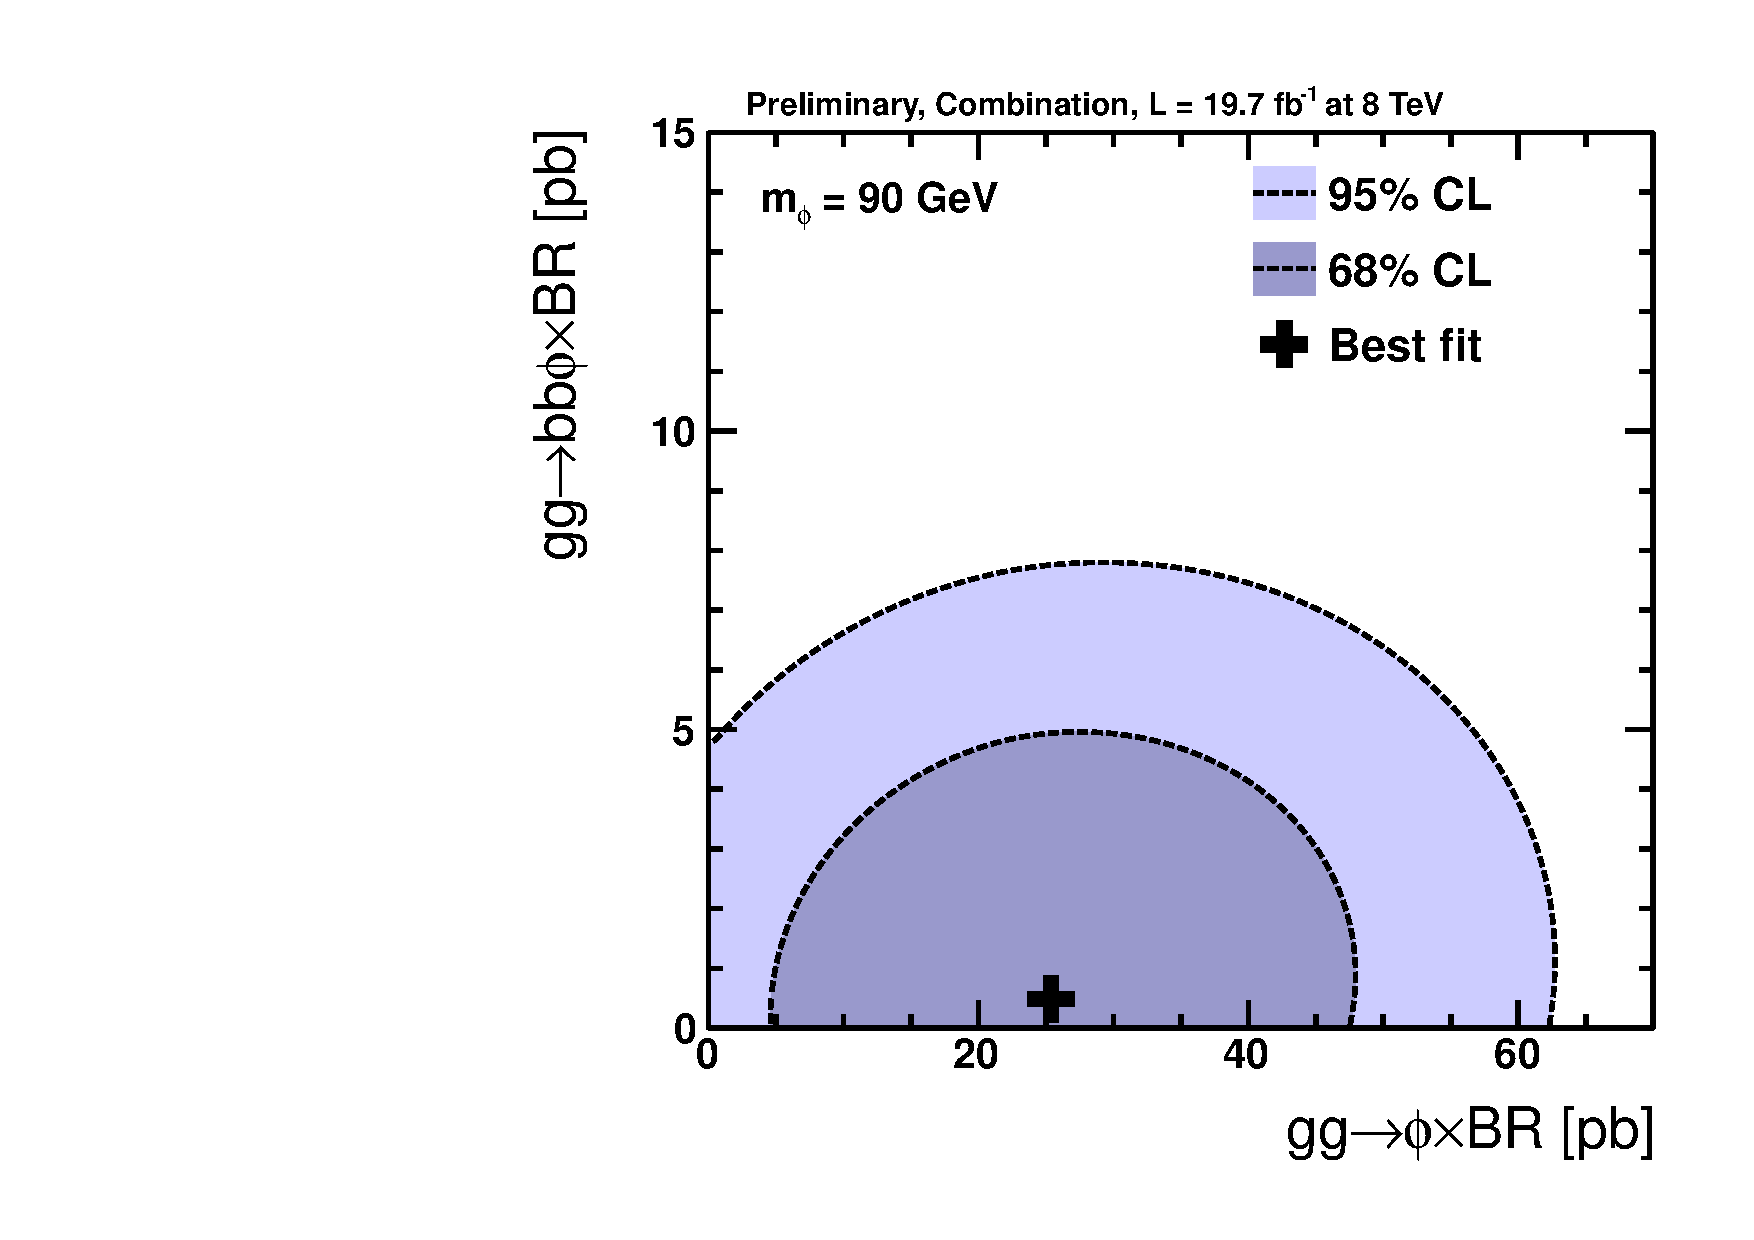
\includegraphics[width=0.45\textwidth]{MSSM/PLOTS/cmb-ggH-bbH-scan-GGH-BBH-90.pdf}
 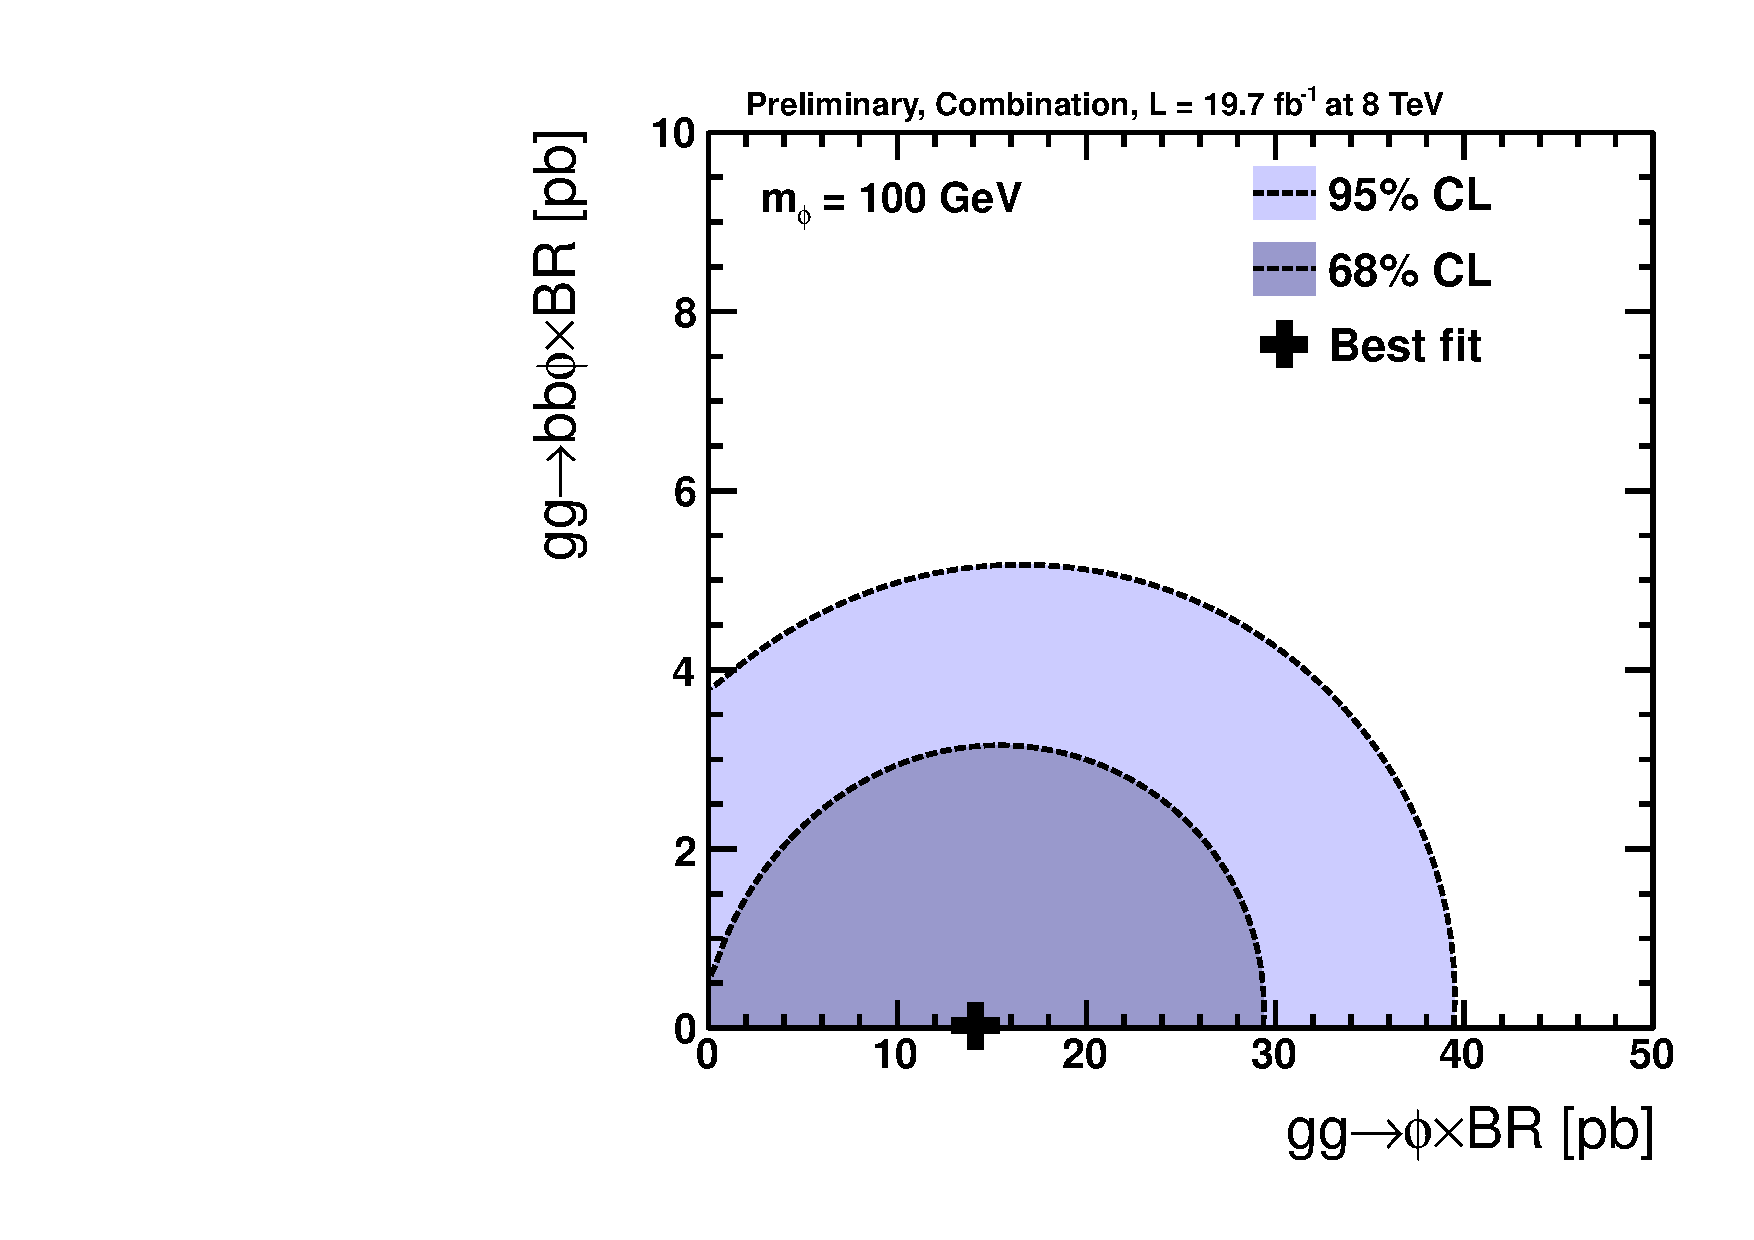
\includegraphics[width=0.45\textwidth]{MSSM/PLOTS/cmb-ggH-bbH-scan-GGH-BBH-100.pdf}
 \caption{Likelihood contours of $\sigma\cdot$BR(gg$\Phi$) and $\sigma\cdot$BR(bb$\Phi$) at 8 TeV center-of-mass energy for different Higgs boson masses}
  \label{fig:contour1}\end{center}\end{figure*}






\begin{figure*}[!h]\begin{center}
 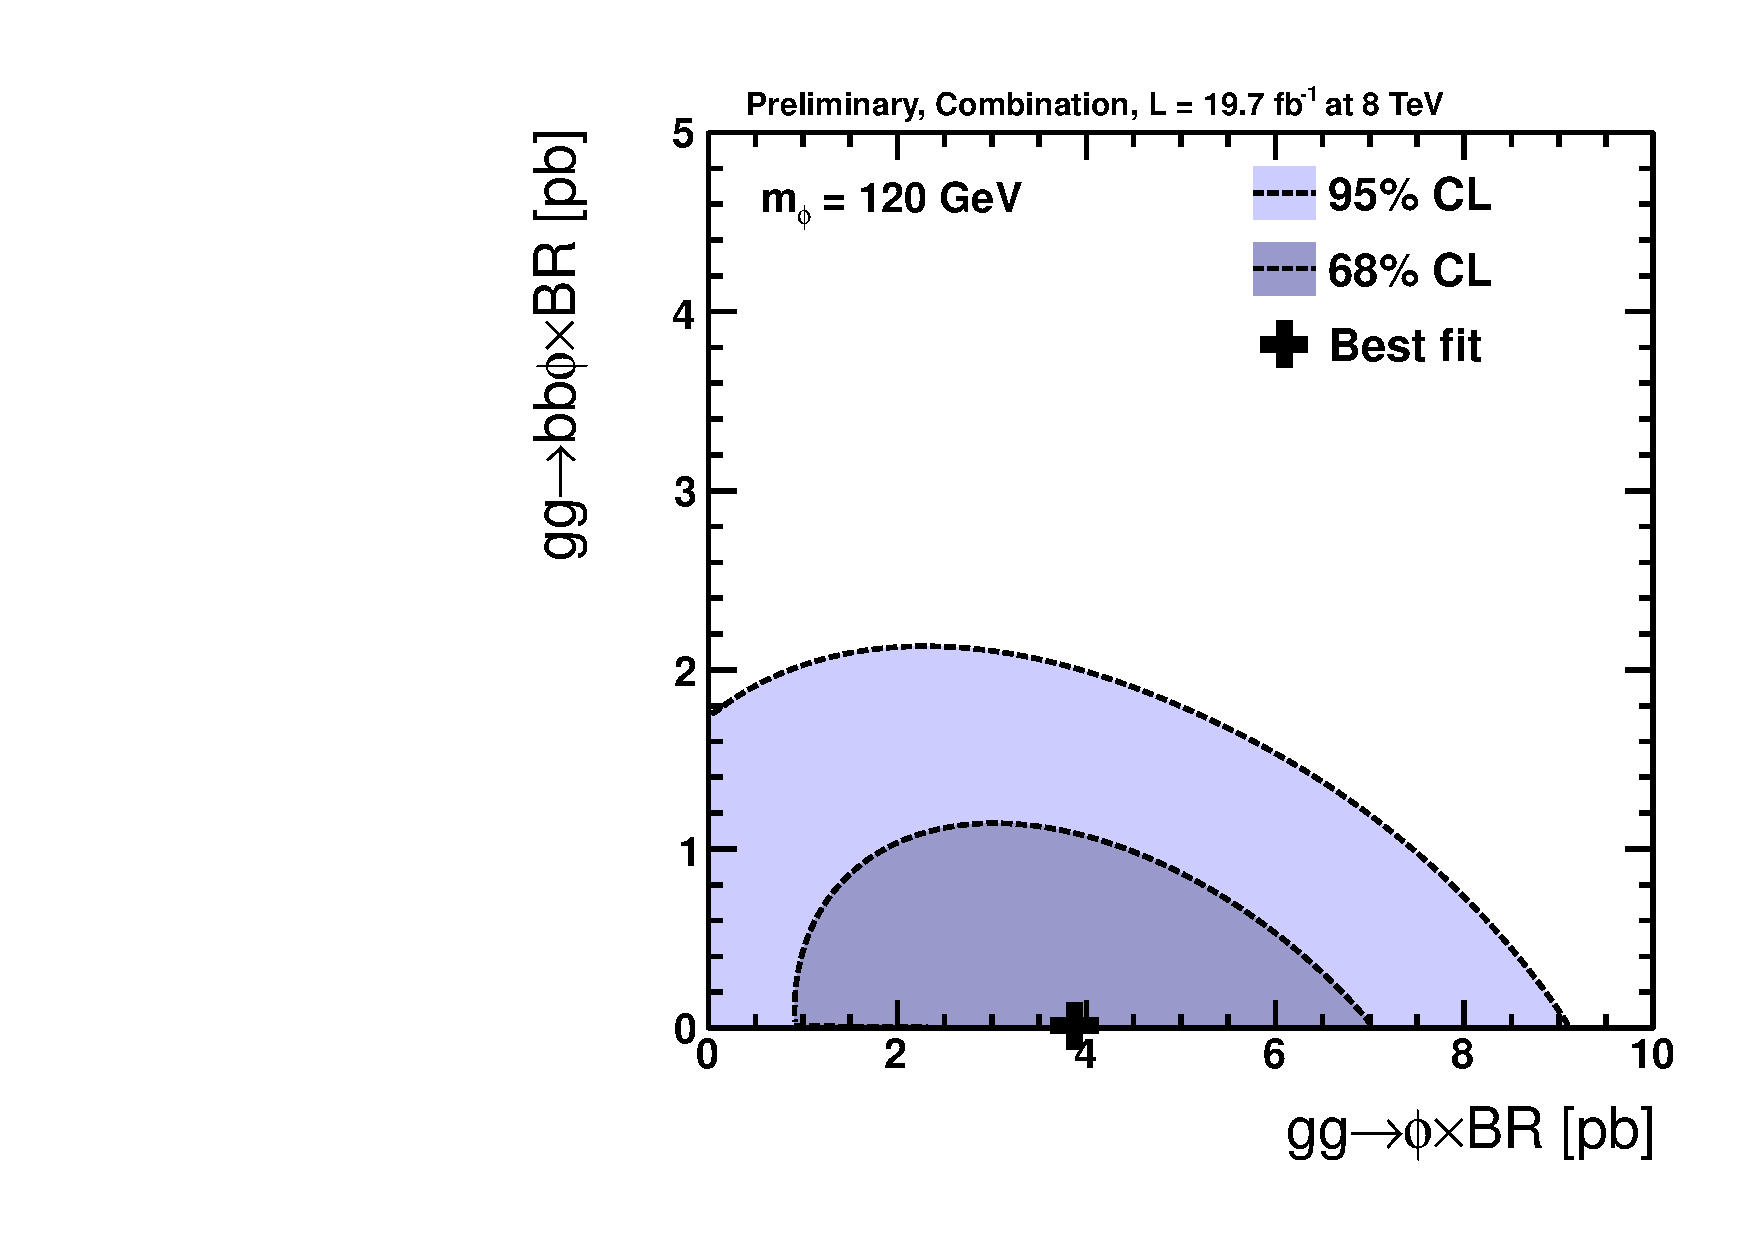
\includegraphics[width=0.45\textwidth]{MSSM/PLOTS/cmb-ggH-bbH-scan-GGH-BBH-120.pdf}
 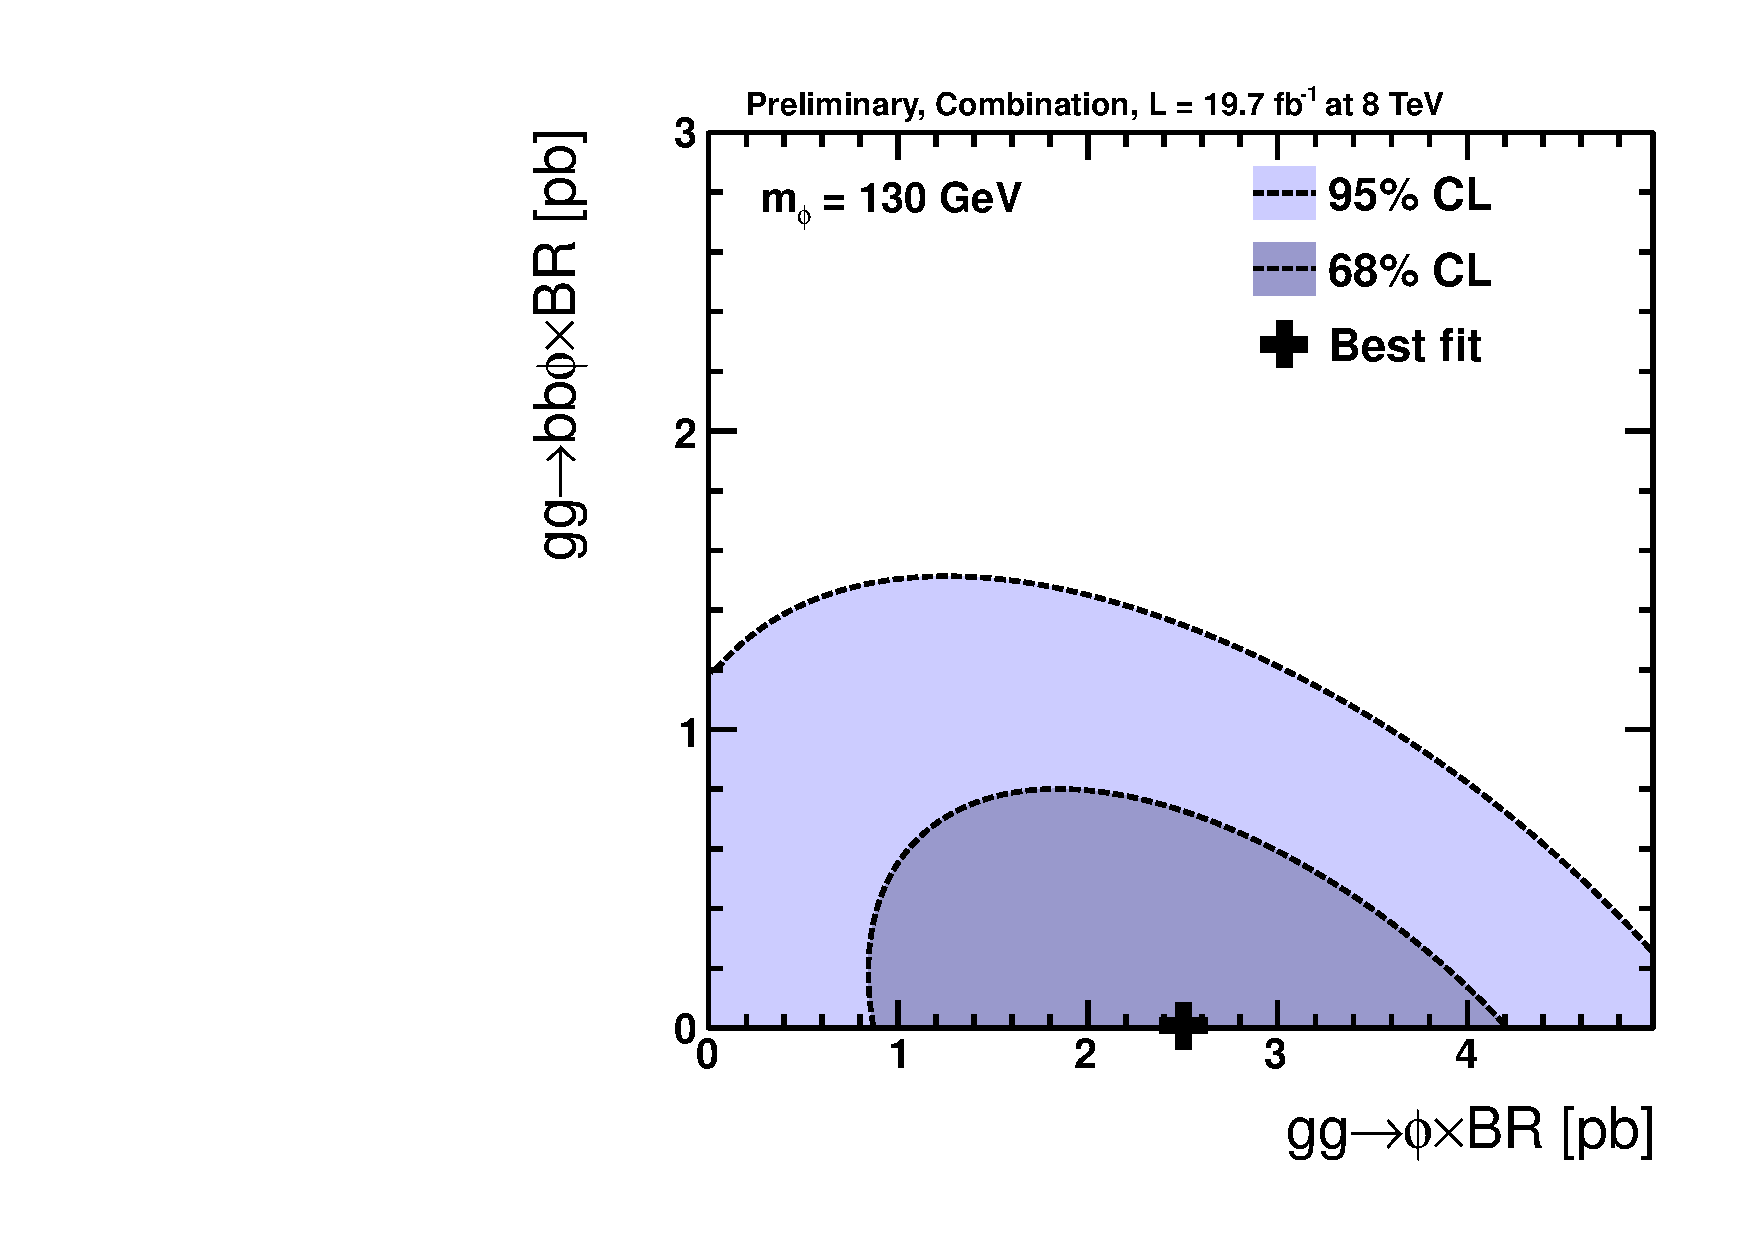
\includegraphics[width=0.45\textwidth]{MSSM/PLOTS/cmb-ggH-bbH-scan-GGH-BBH-130.pdf}
 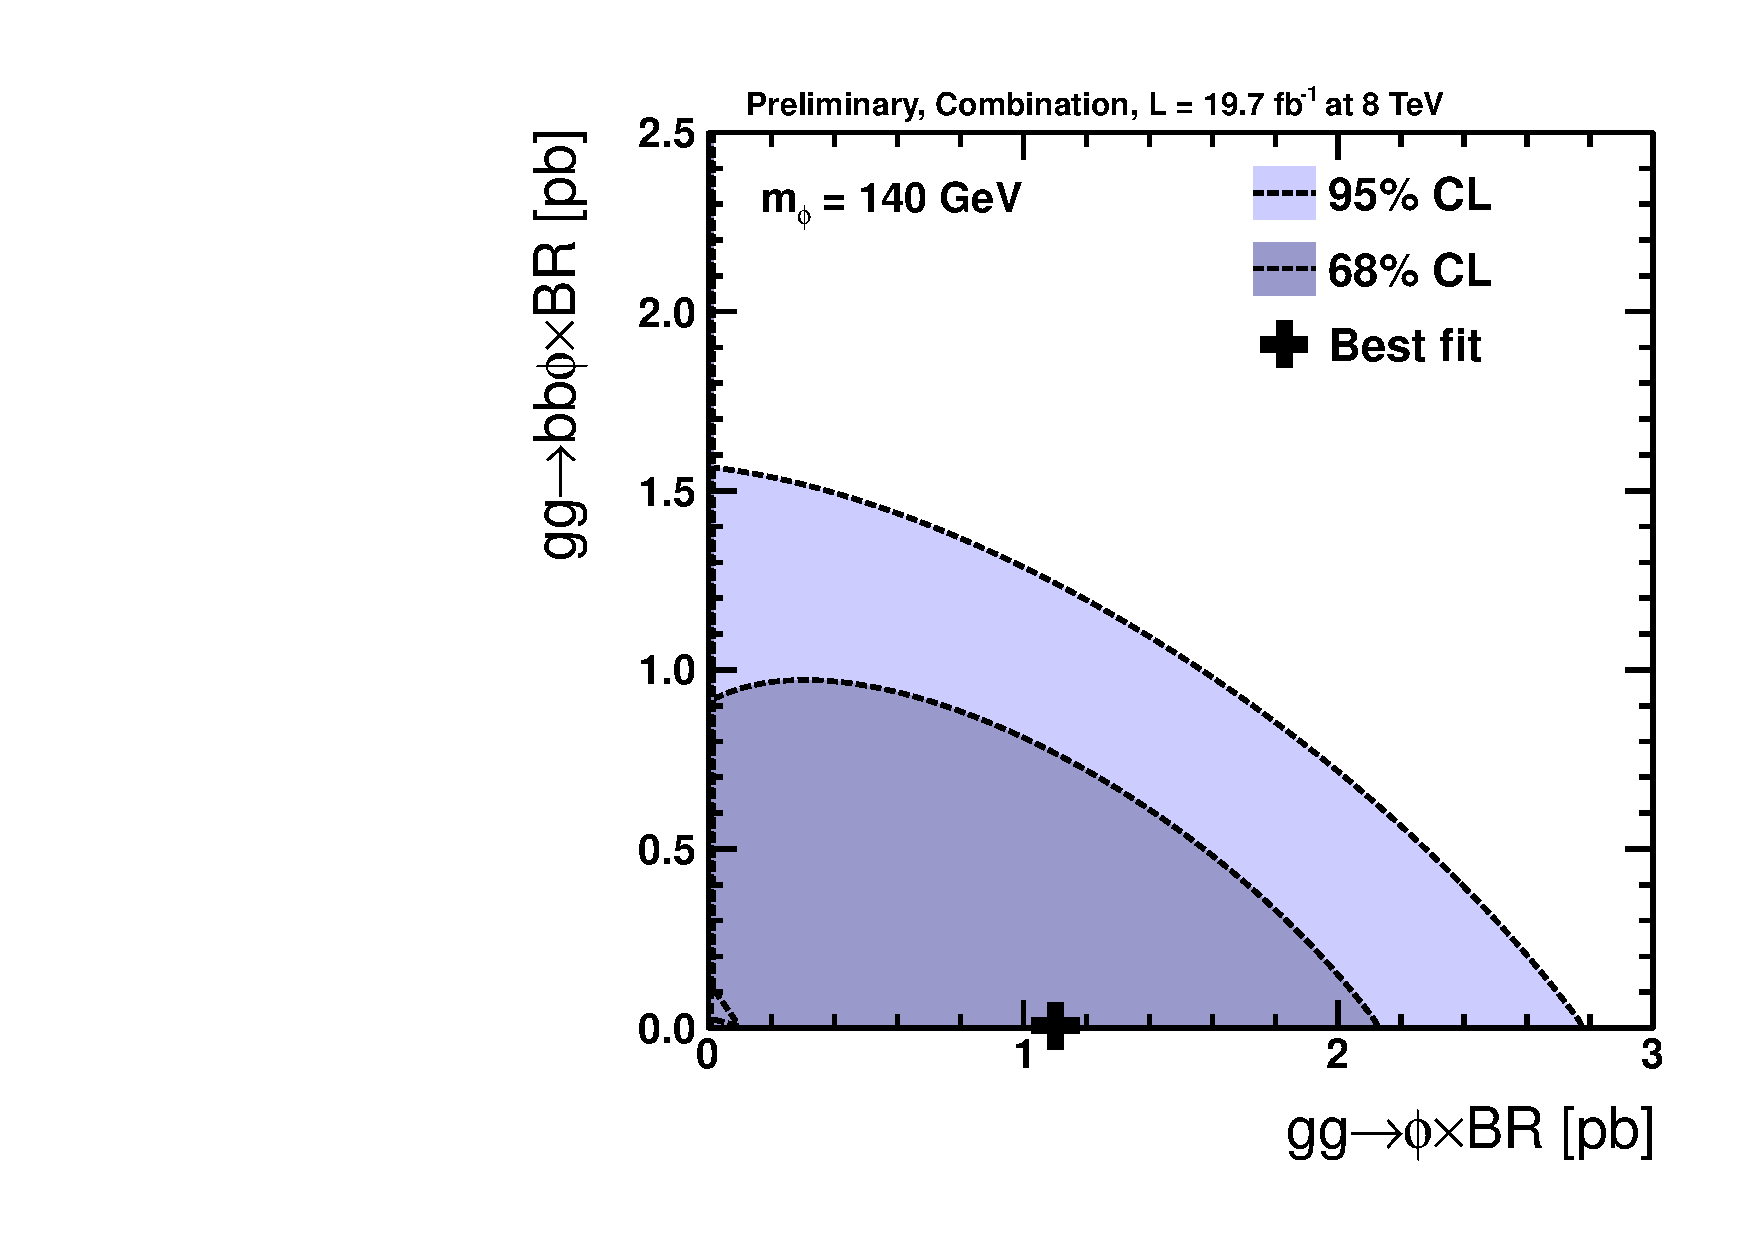
\includegraphics[width=0.45\textwidth]{MSSM/PLOTS/cmb-ggH-bbH-scan-GGH-BBH-140.pdf}
 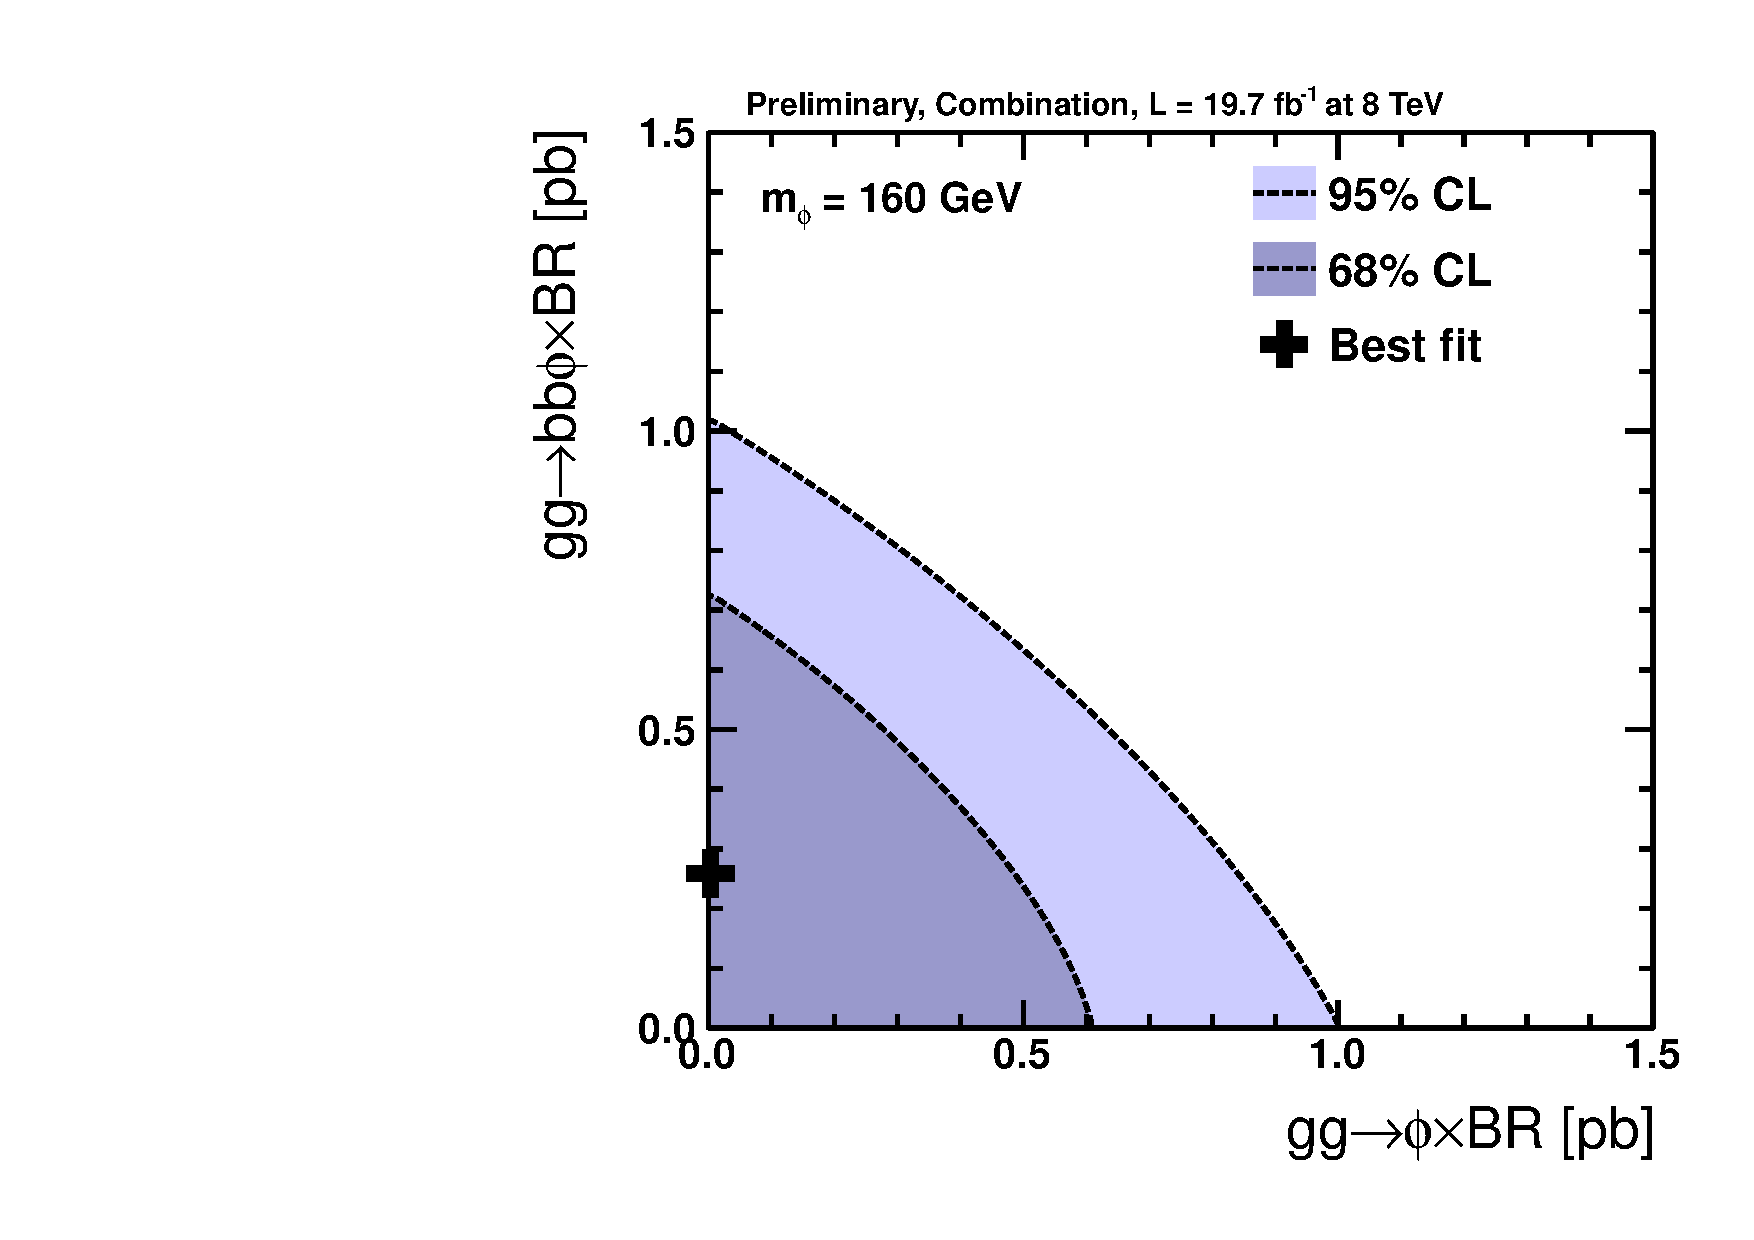
\includegraphics[width=0.45\textwidth]{MSSM/PLOTS/cmb-ggH-bbH-scan-GGH-BBH-160.pdf}
 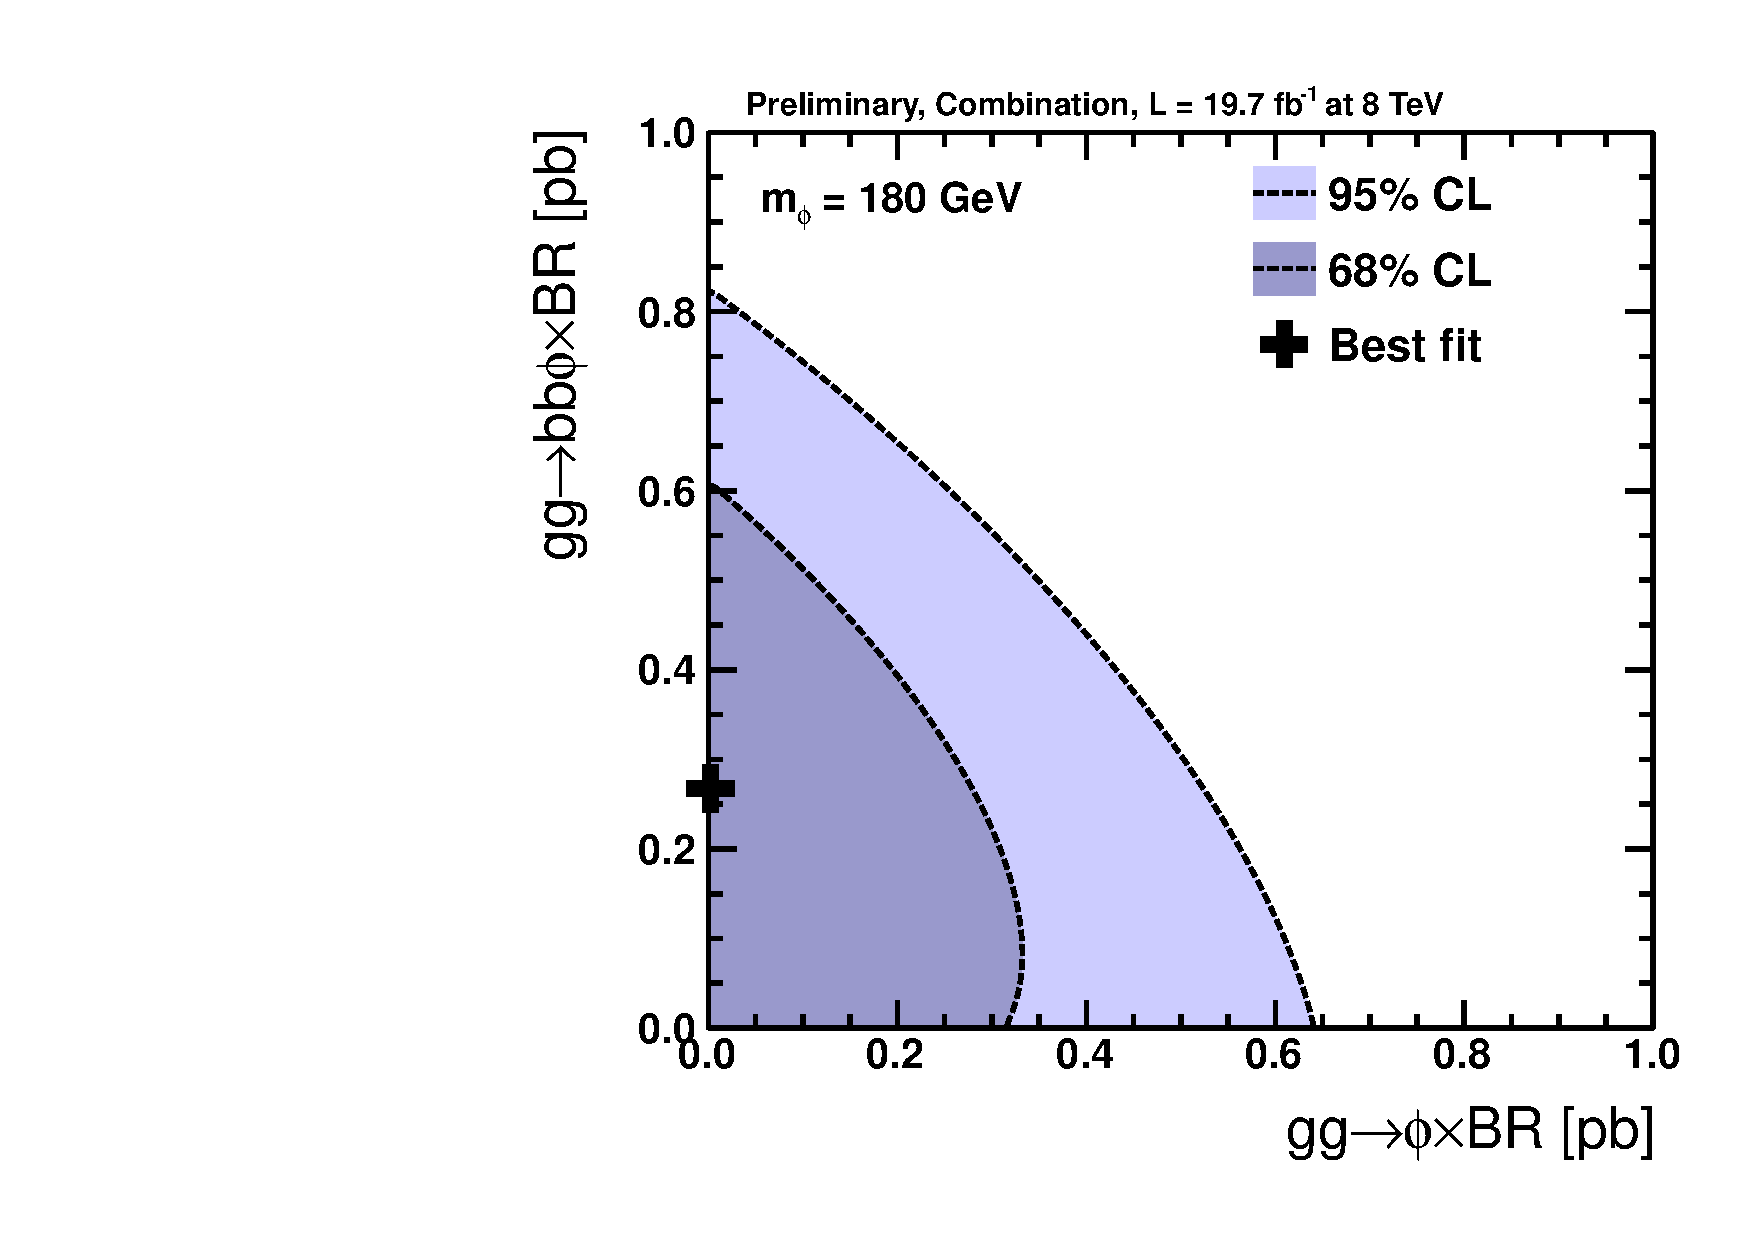
\includegraphics[width=0.45\textwidth]{MSSM/PLOTS/cmb-ggH-bbH-scan-GGH-BBH-180.pdf}
 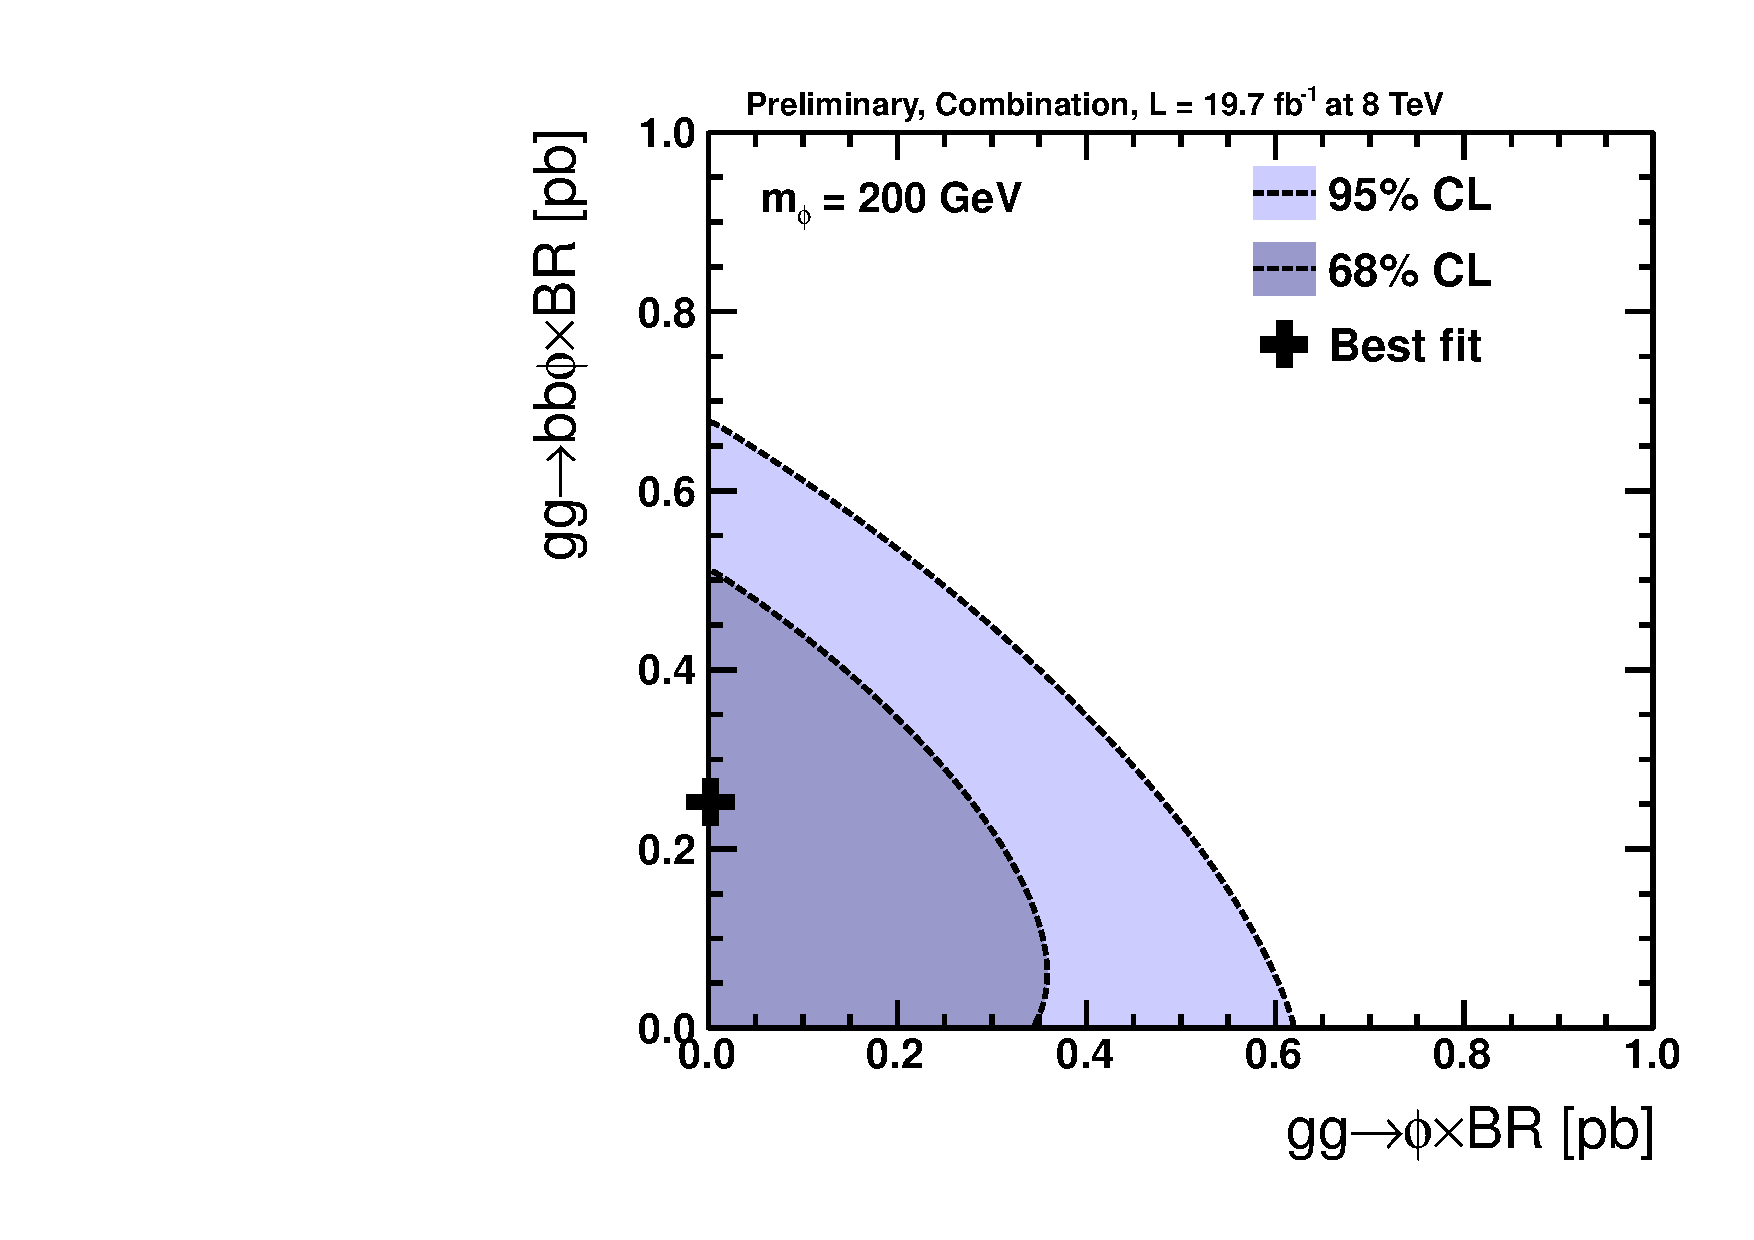
\includegraphics[width=0.45\textwidth]{MSSM/PLOTS/cmb-ggH-bbH-scan-GGH-BBH-200.pdf}
 \caption{Likelihood contours of $\sigma\cdot$BR(gg$\Phi$) and $\sigma\cdot$BR(bb$\Phi$) at 8 TeV center-of-mass energy for different Higgs boson masses}
  \label{fig:contour2}\end{center}\end{figure*}


\begin{figure*}[!h]\begin{center}
 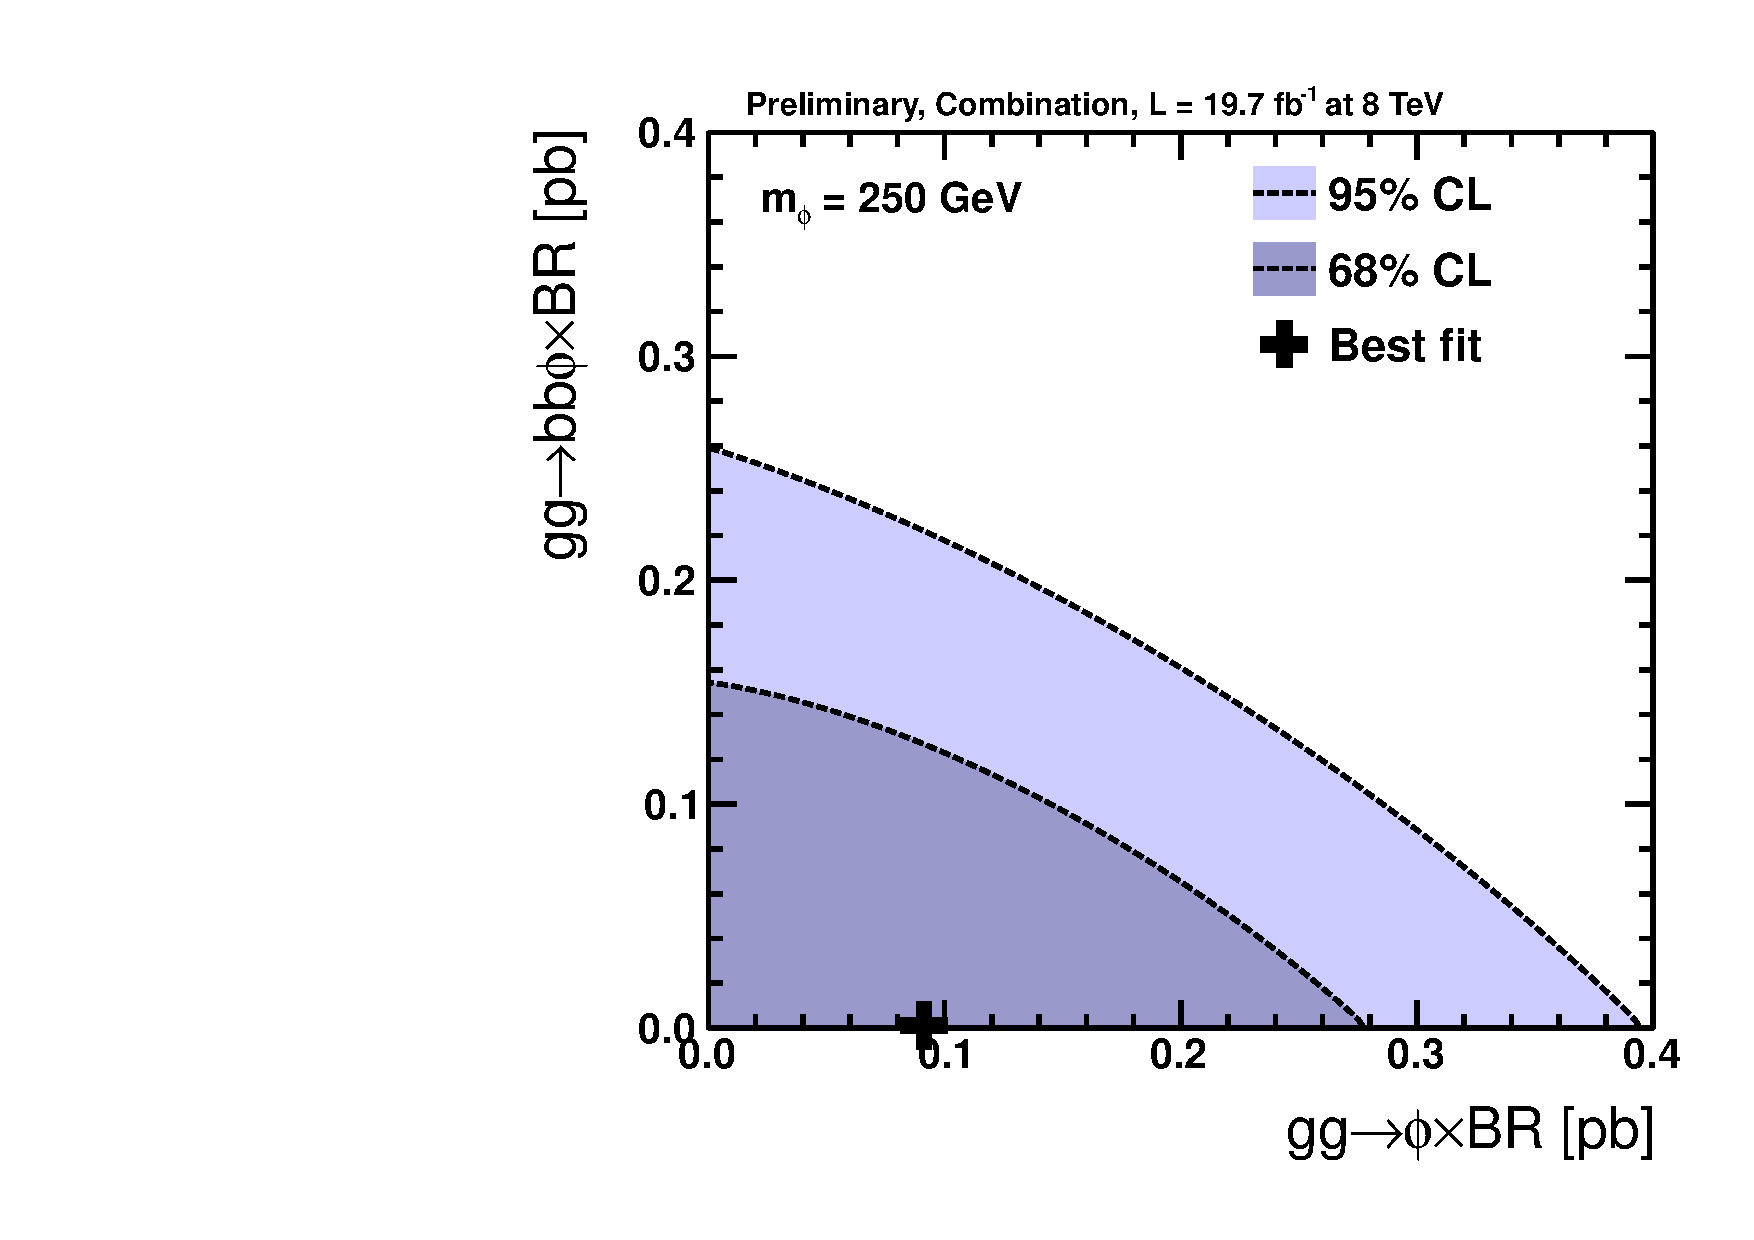
\includegraphics[width=0.45\textwidth]{MSSM/PLOTS/cmb-ggH-bbH-scan-GGH-BBH-250.pdf}
 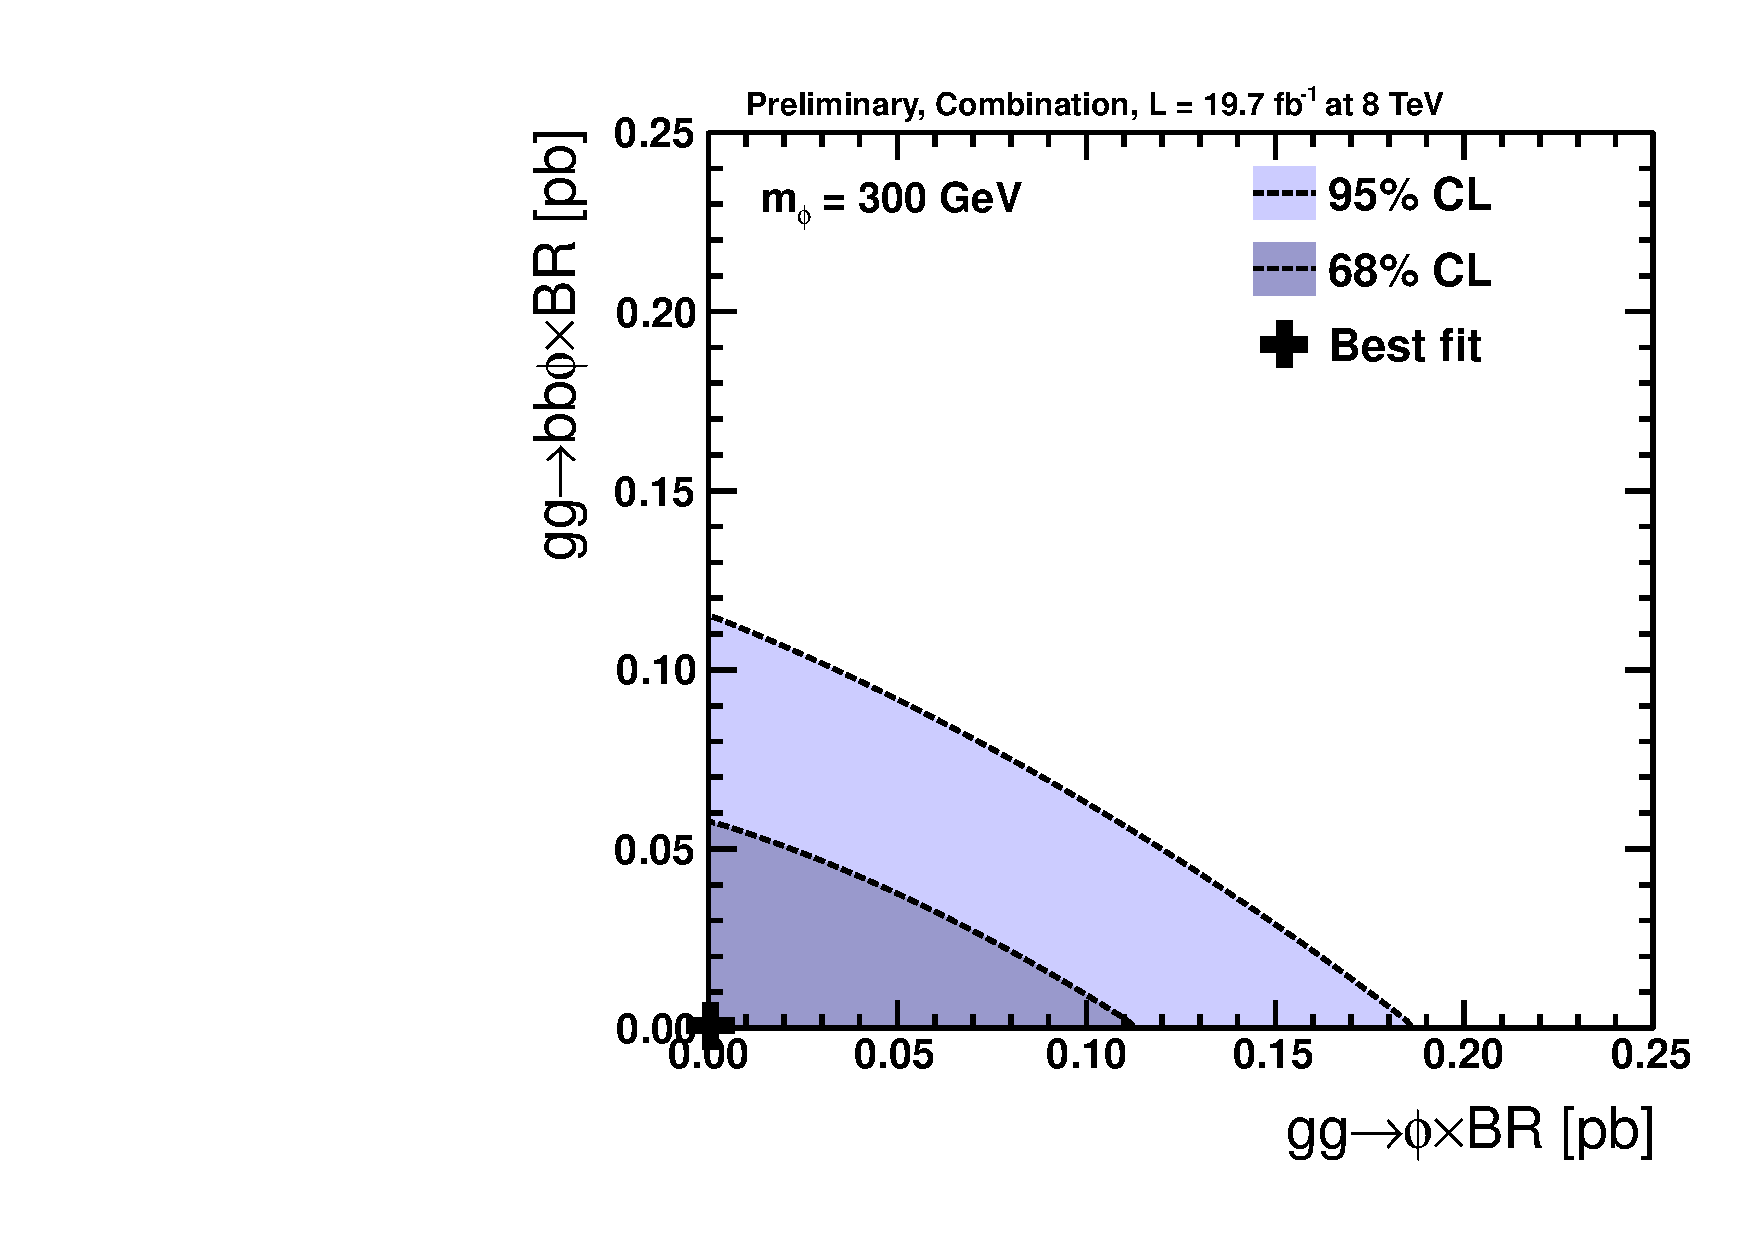
\includegraphics[width=0.45\textwidth]{MSSM/PLOTS/cmb-ggH-bbH-scan-GGH-BBH-300.pdf}
 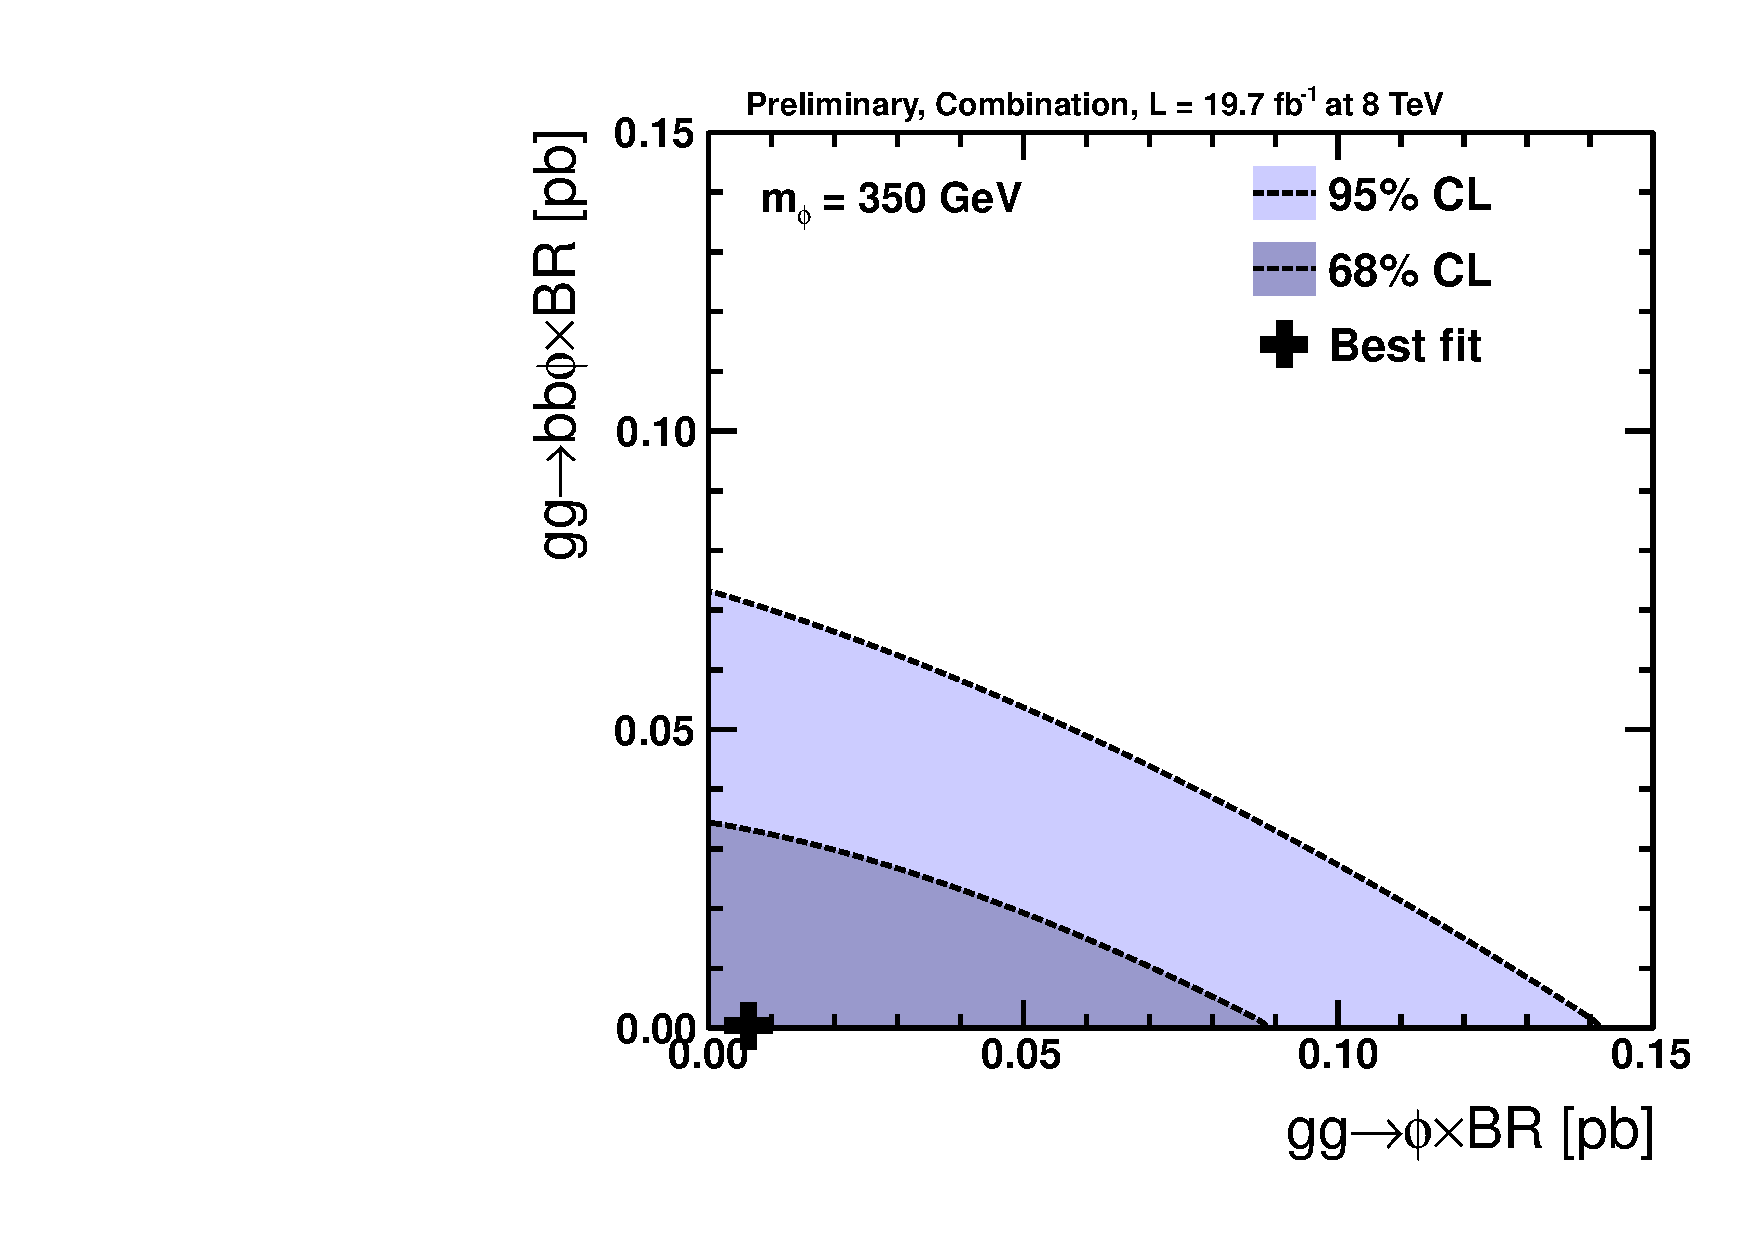
\includegraphics[width=0.45\textwidth]{MSSM/PLOTS/cmb-ggH-bbH-scan-GGH-BBH-350.pdf}
 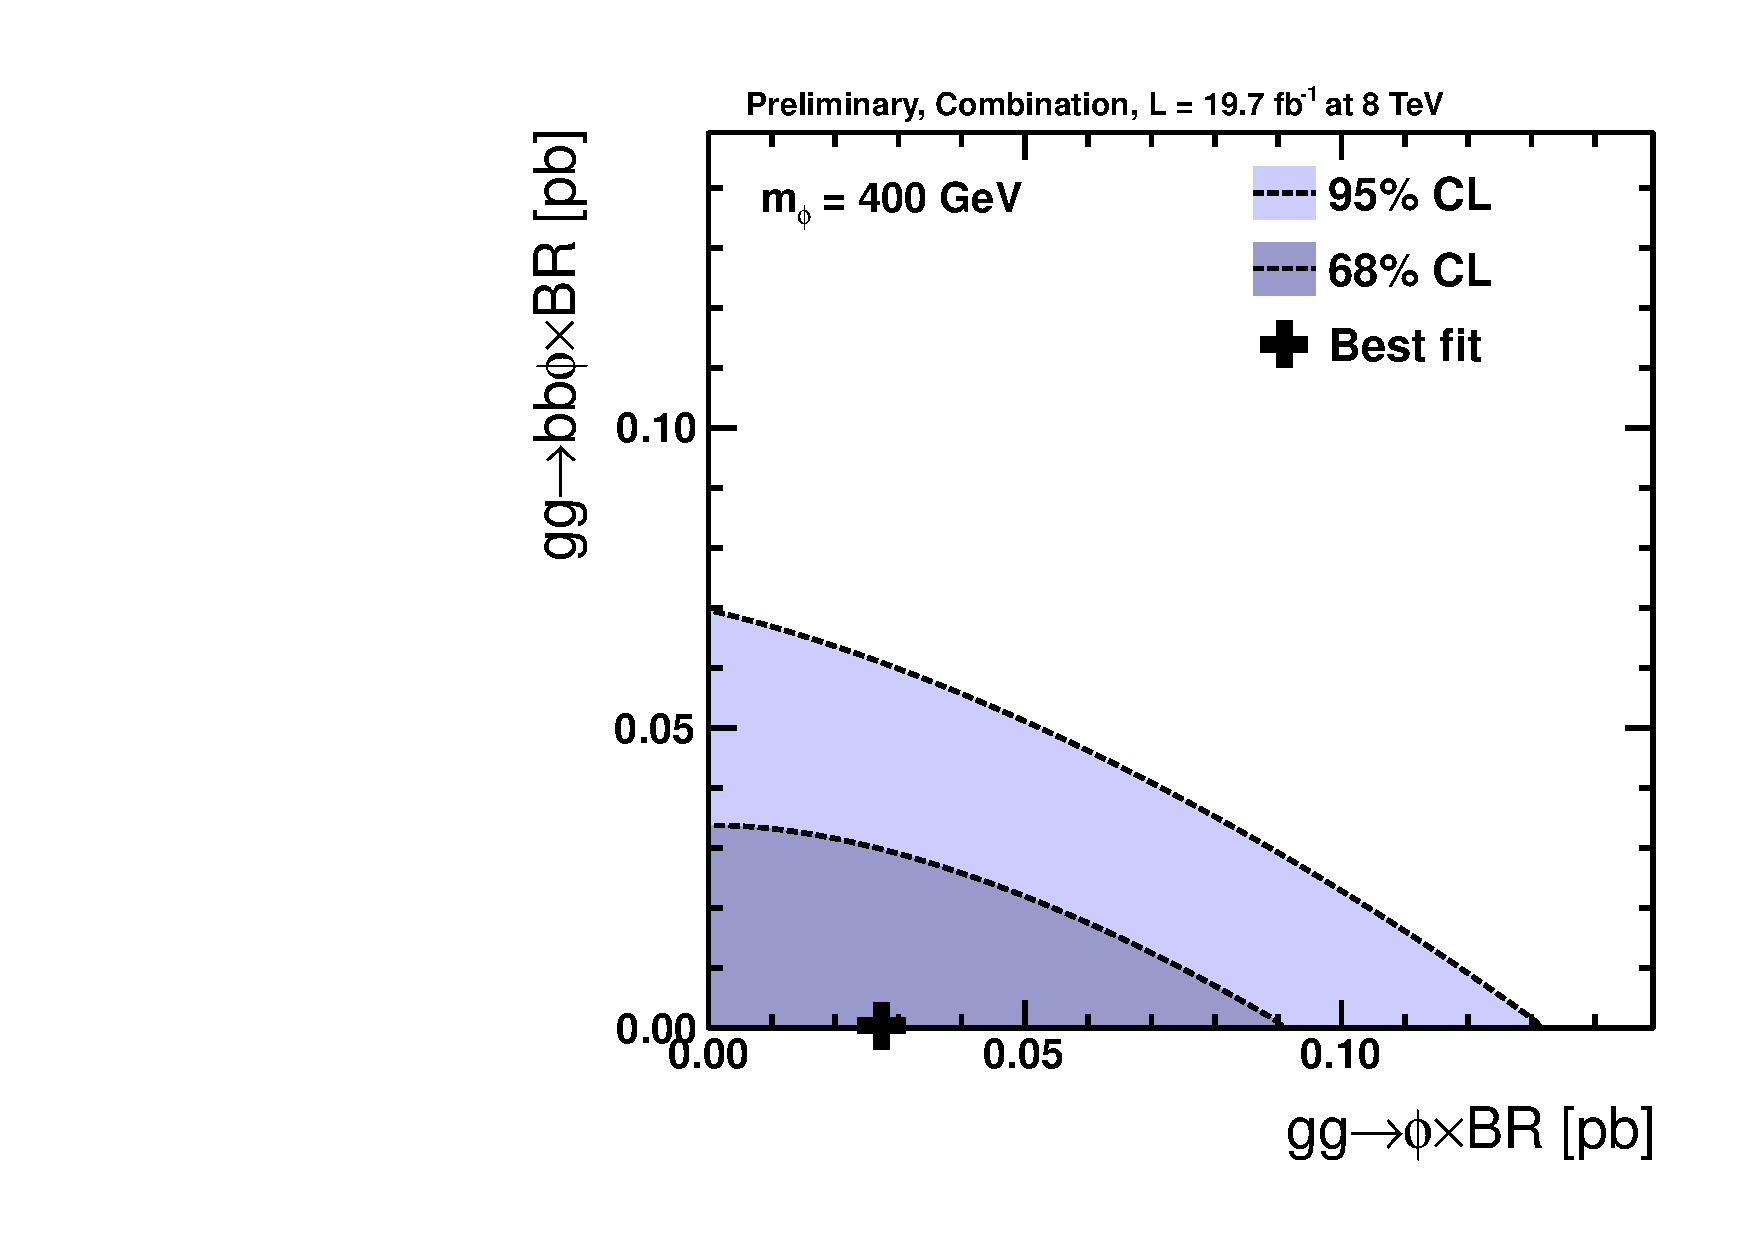
\includegraphics[width=0.45\textwidth]{MSSM/PLOTS/cmb-ggH-bbH-scan-GGH-BBH-400.pdf}
 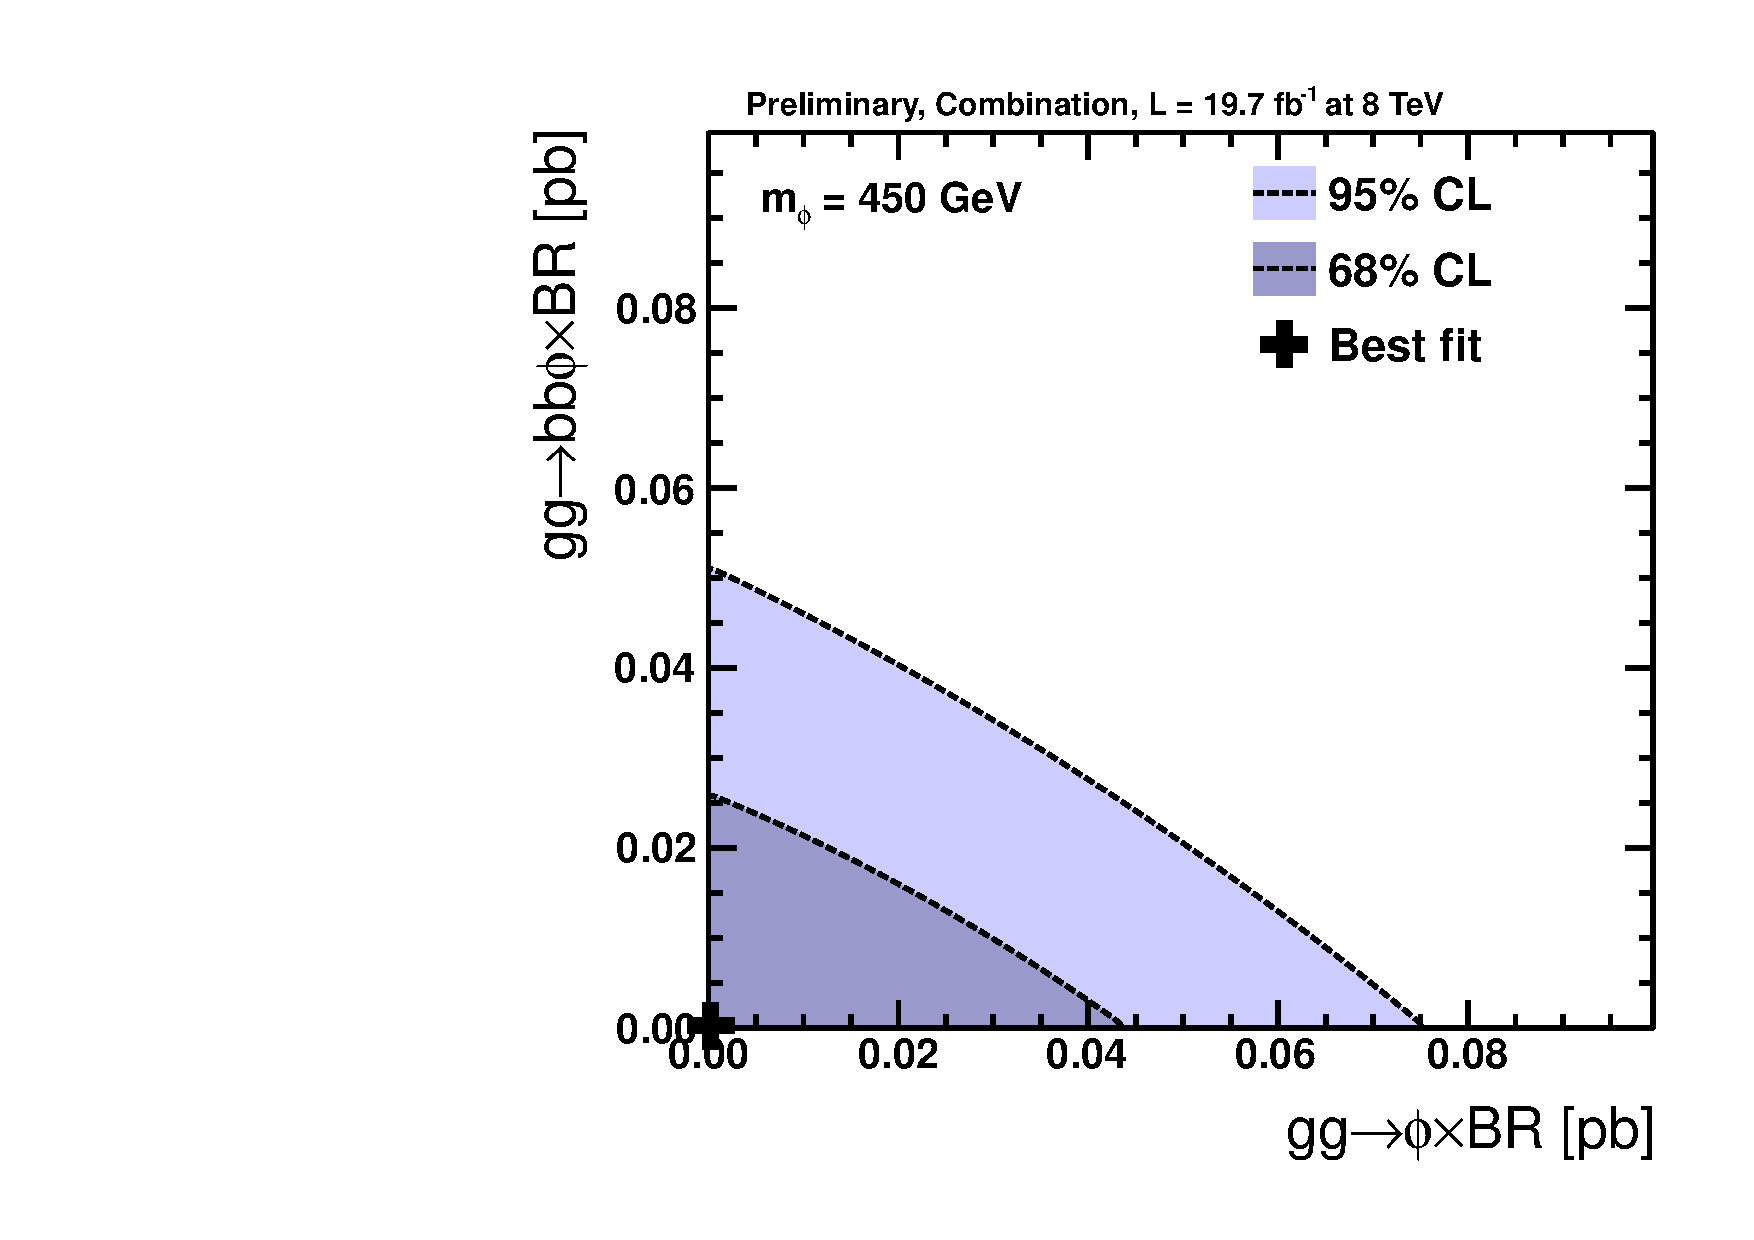
\includegraphics[width=0.45\textwidth]{MSSM/PLOTS/cmb-ggH-bbH-scan-GGH-BBH-450.pdf}
 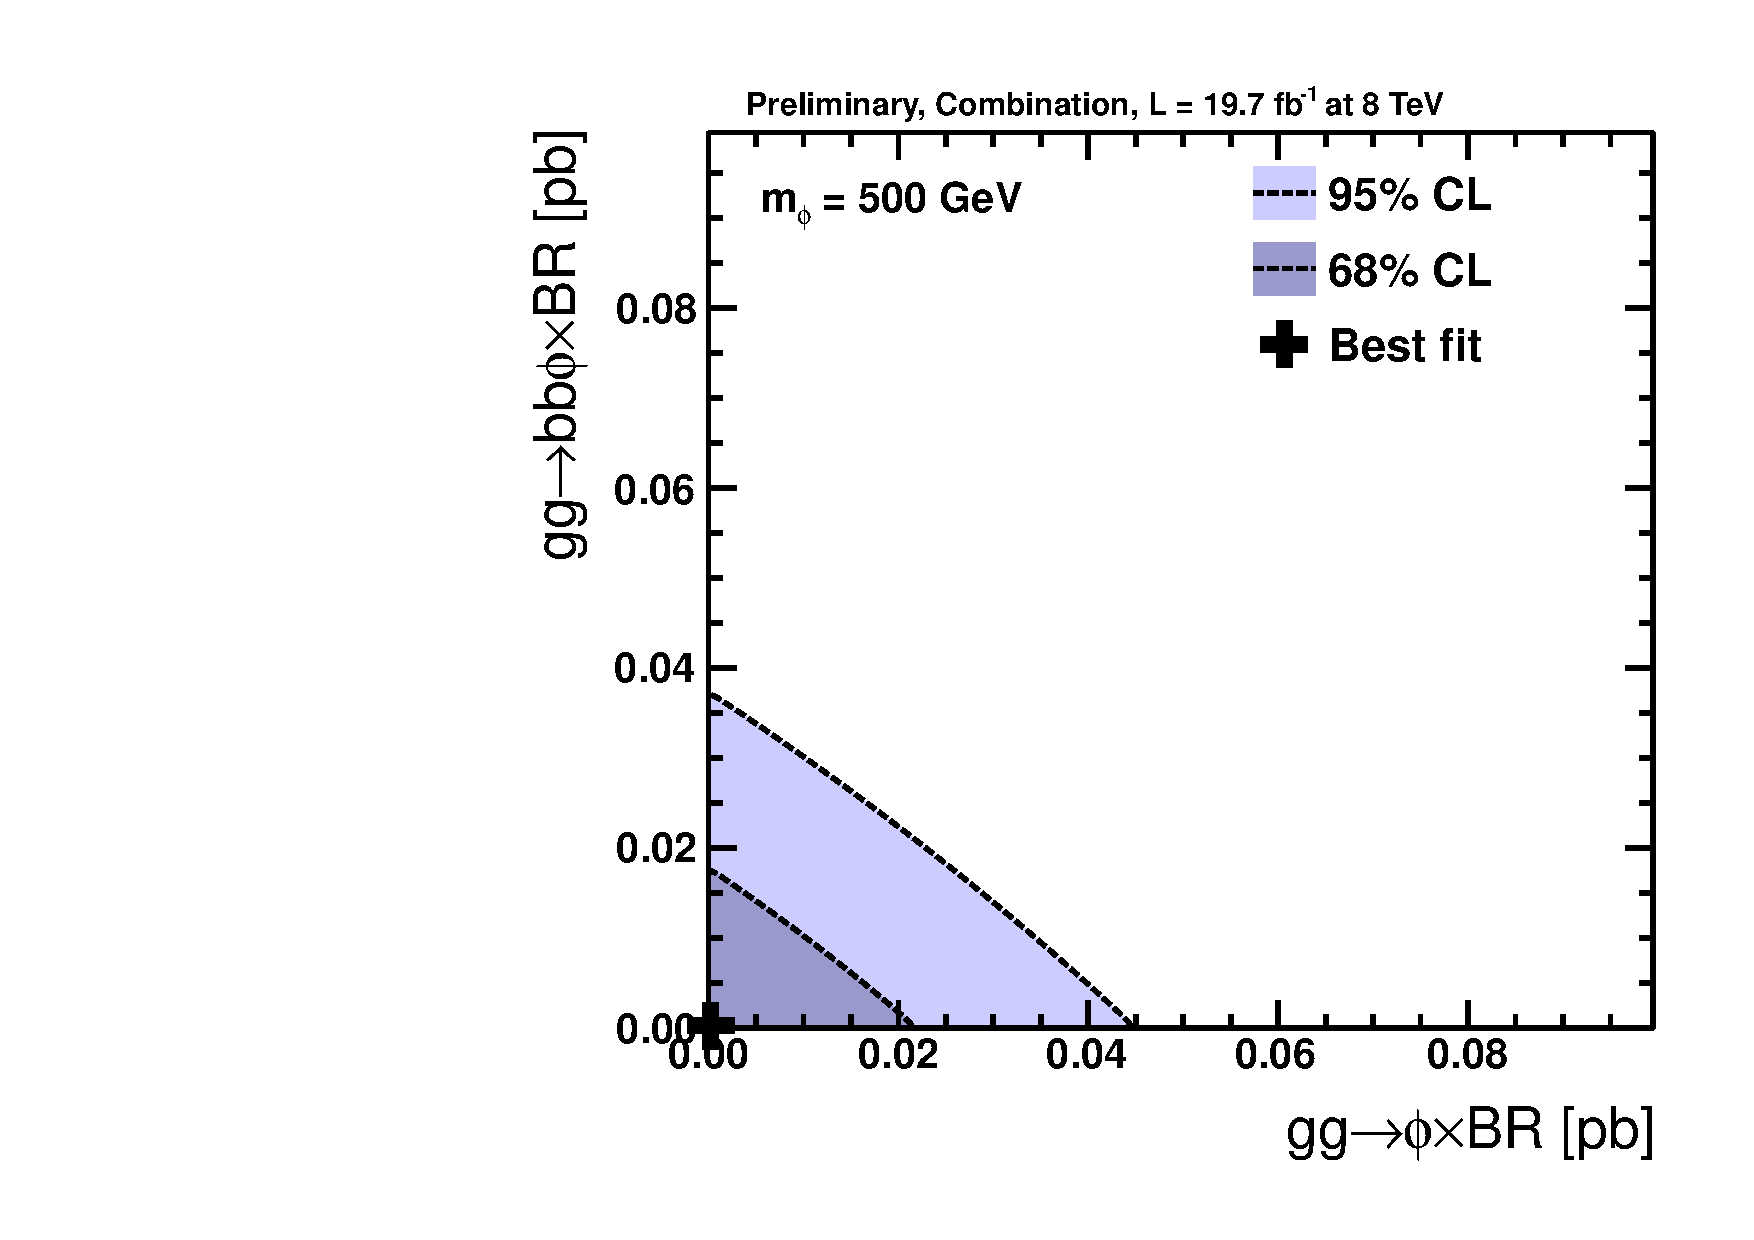
\includegraphics[width=0.45\textwidth]{MSSM/PLOTS/cmb-ggH-bbH-scan-GGH-BBH-500.pdf}
 \caption{Likelihood contours of $\sigma\cdot$BR(gg$\Phi$) and $\sigma\cdot$BR(bb$\Phi$) at 8 TeV center-of-mass energy for different Higgs boson masses}
  \label{fig:contour3}\end{center}\end{figure*}


\begin{figure*}[!h]\begin{center}
 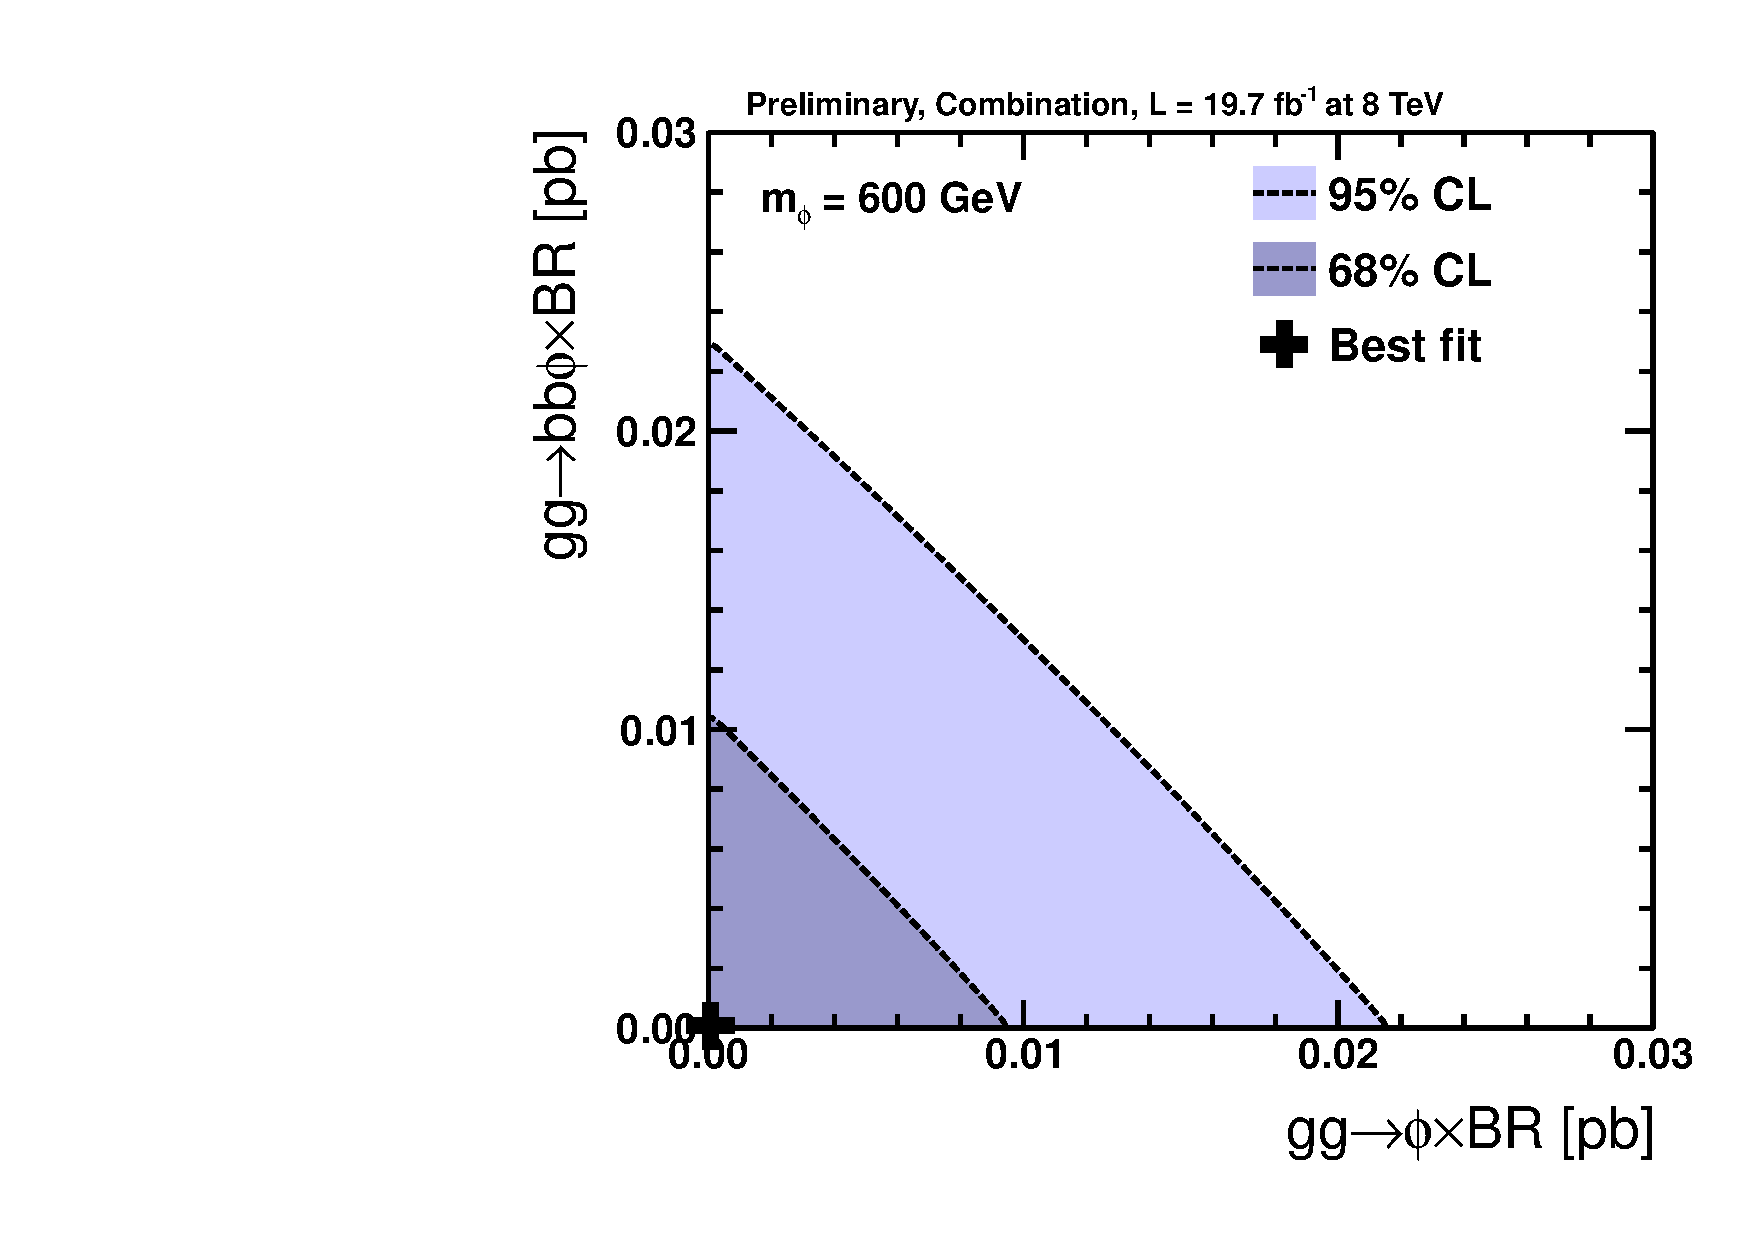
\includegraphics[width=0.45\textwidth]{MSSM/PLOTS/cmb-ggH-bbH-scan-GGH-BBH-600.pdf}
 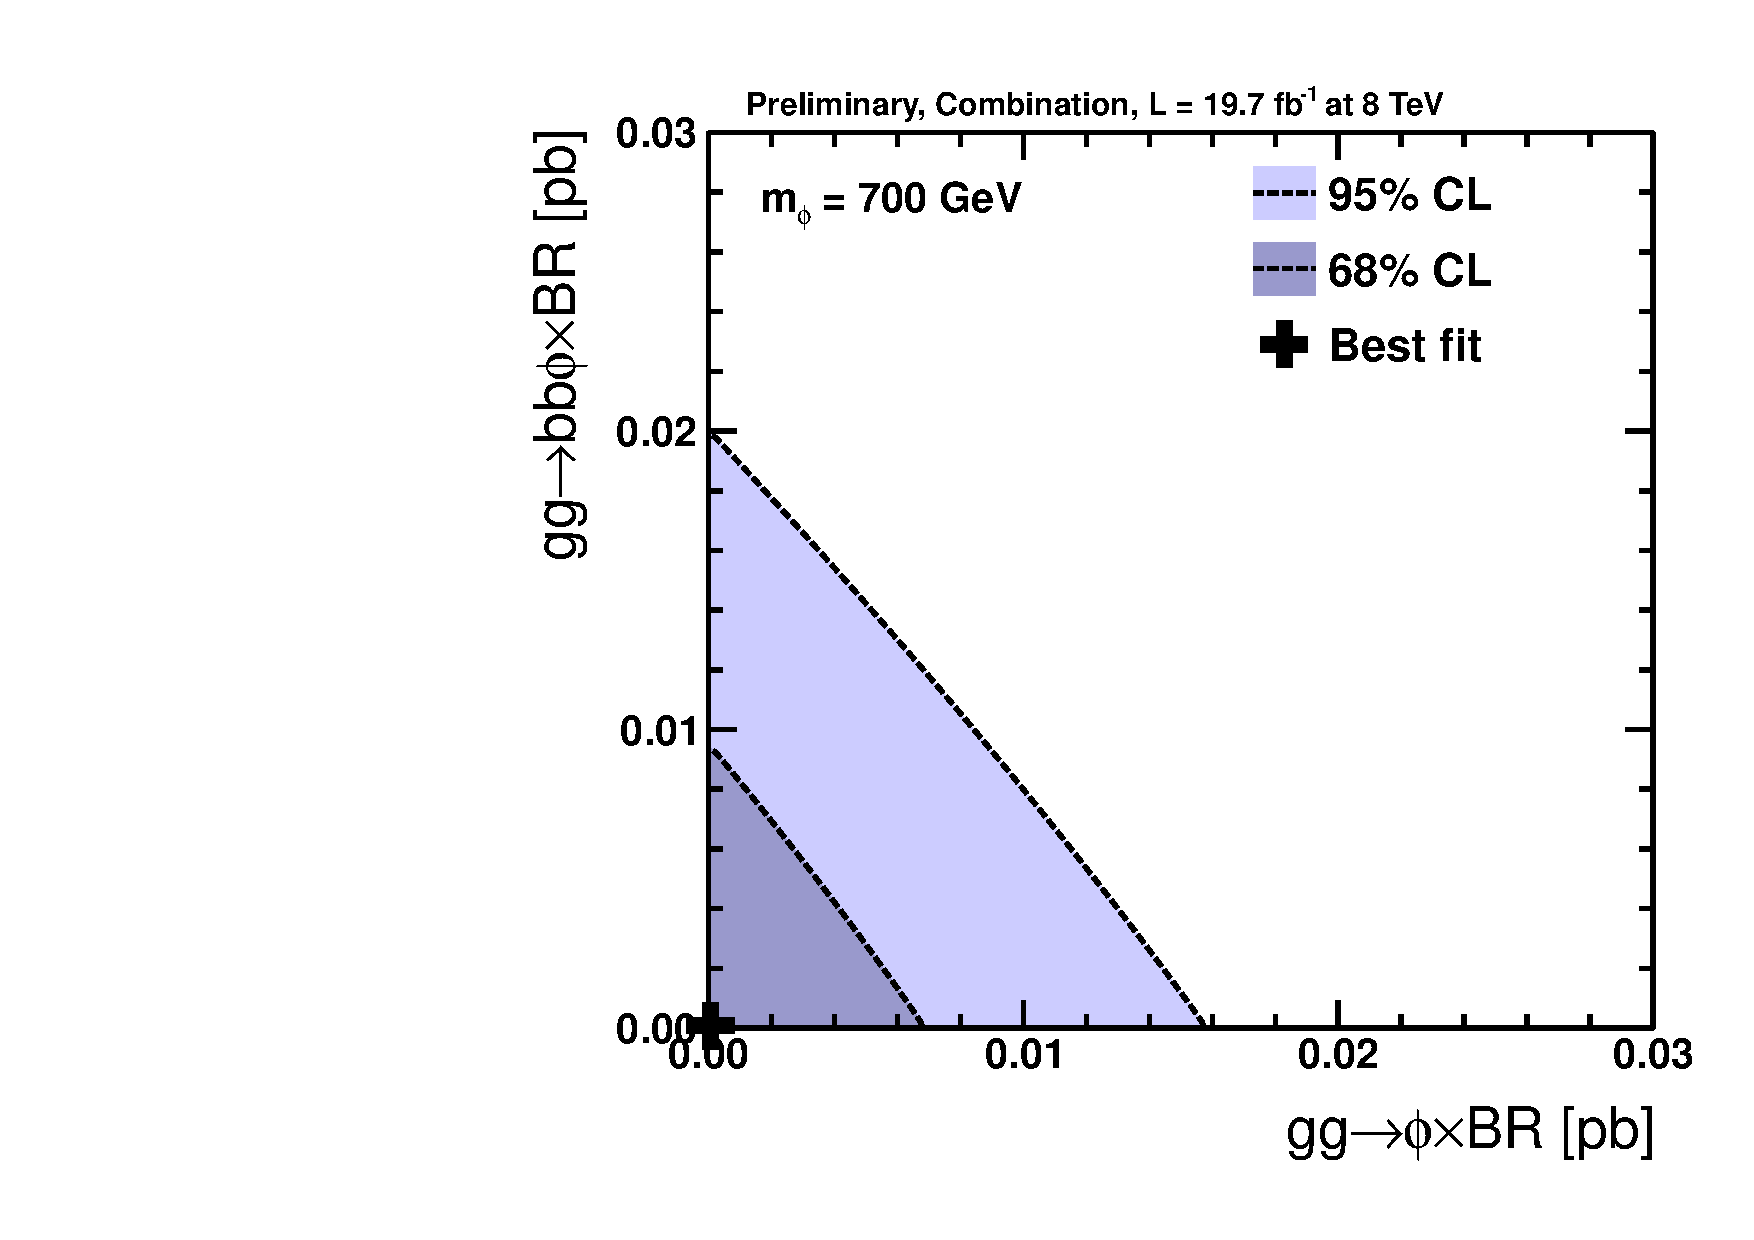
\includegraphics[width=0.45\textwidth]{MSSM/PLOTS/cmb-ggH-bbH-scan-GGH-BBH-700.pdf}
 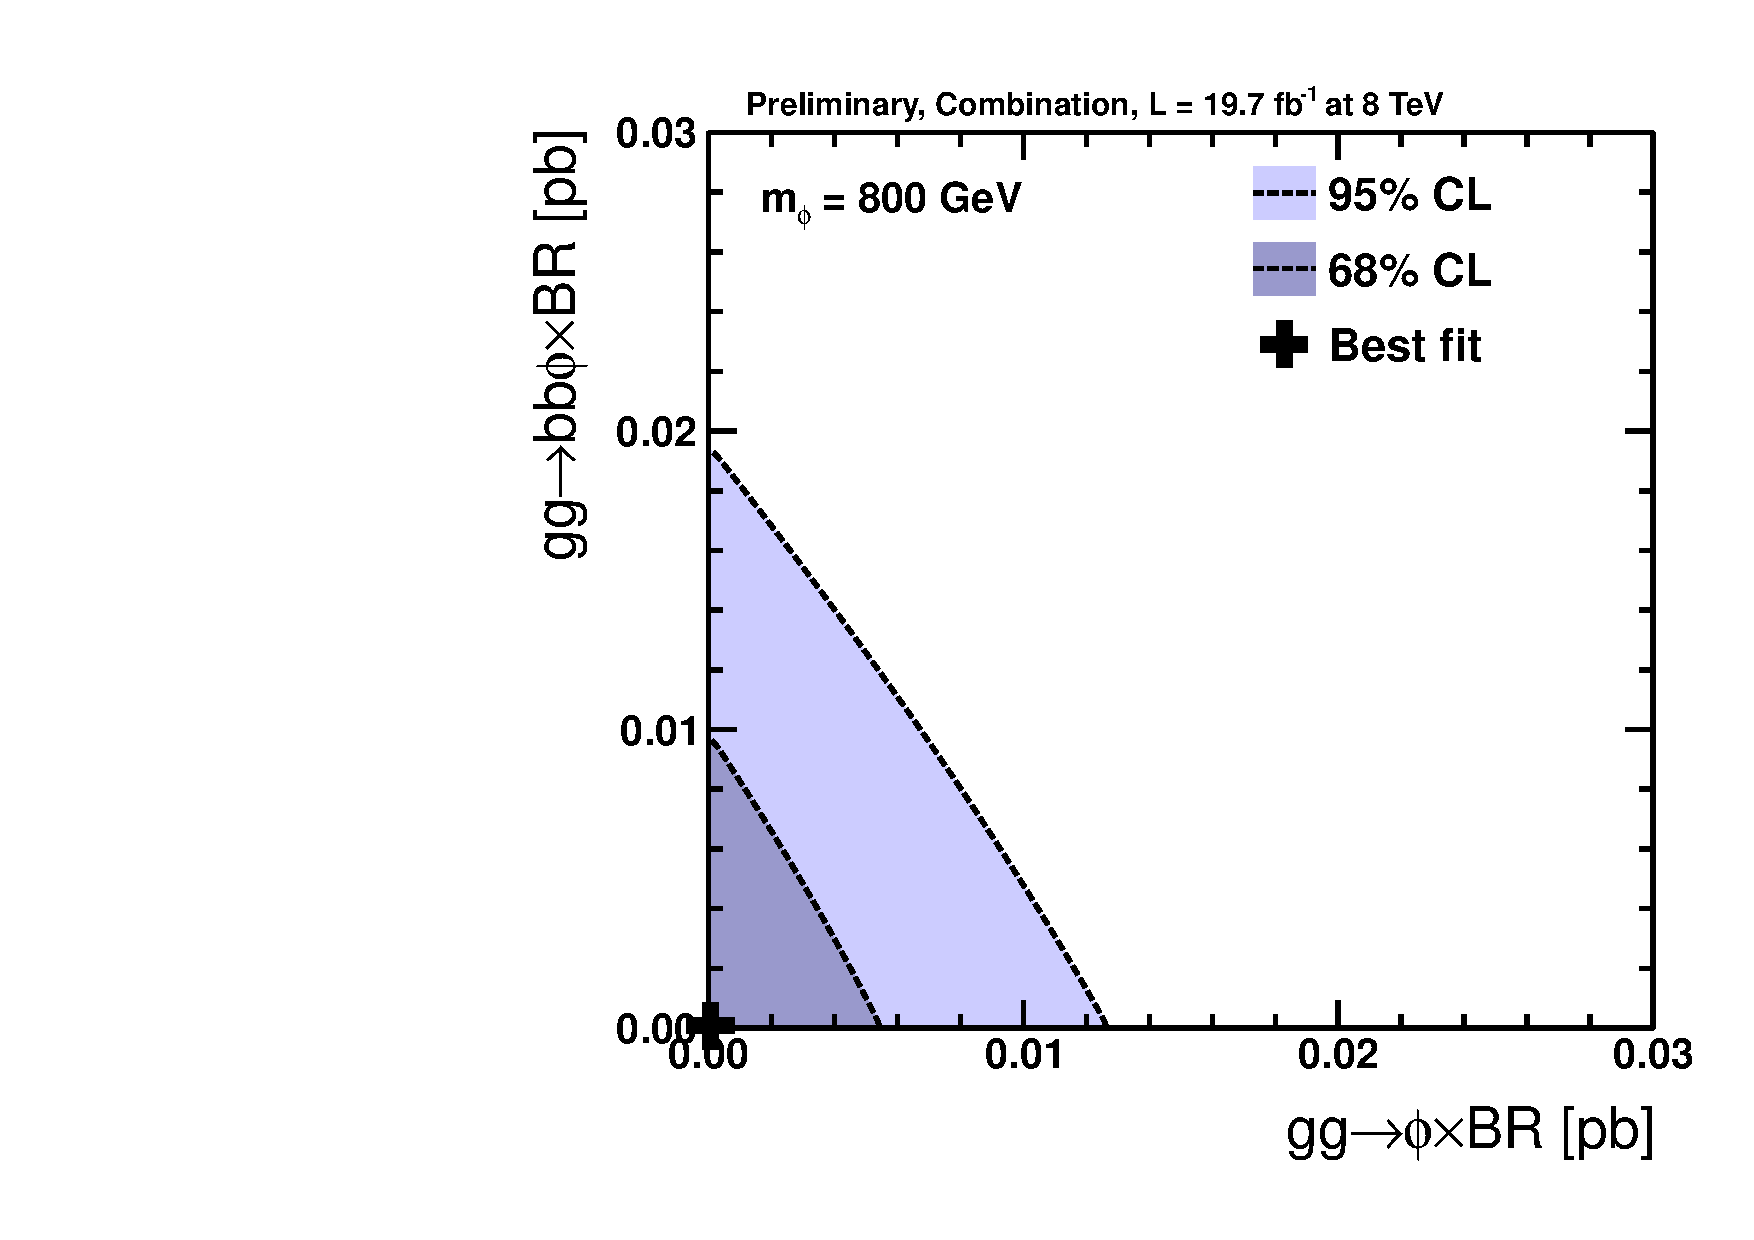
\includegraphics[width=0.45\textwidth]{MSSM/PLOTS/cmb-ggH-bbH-scan-GGH-BBH-800.pdf}
 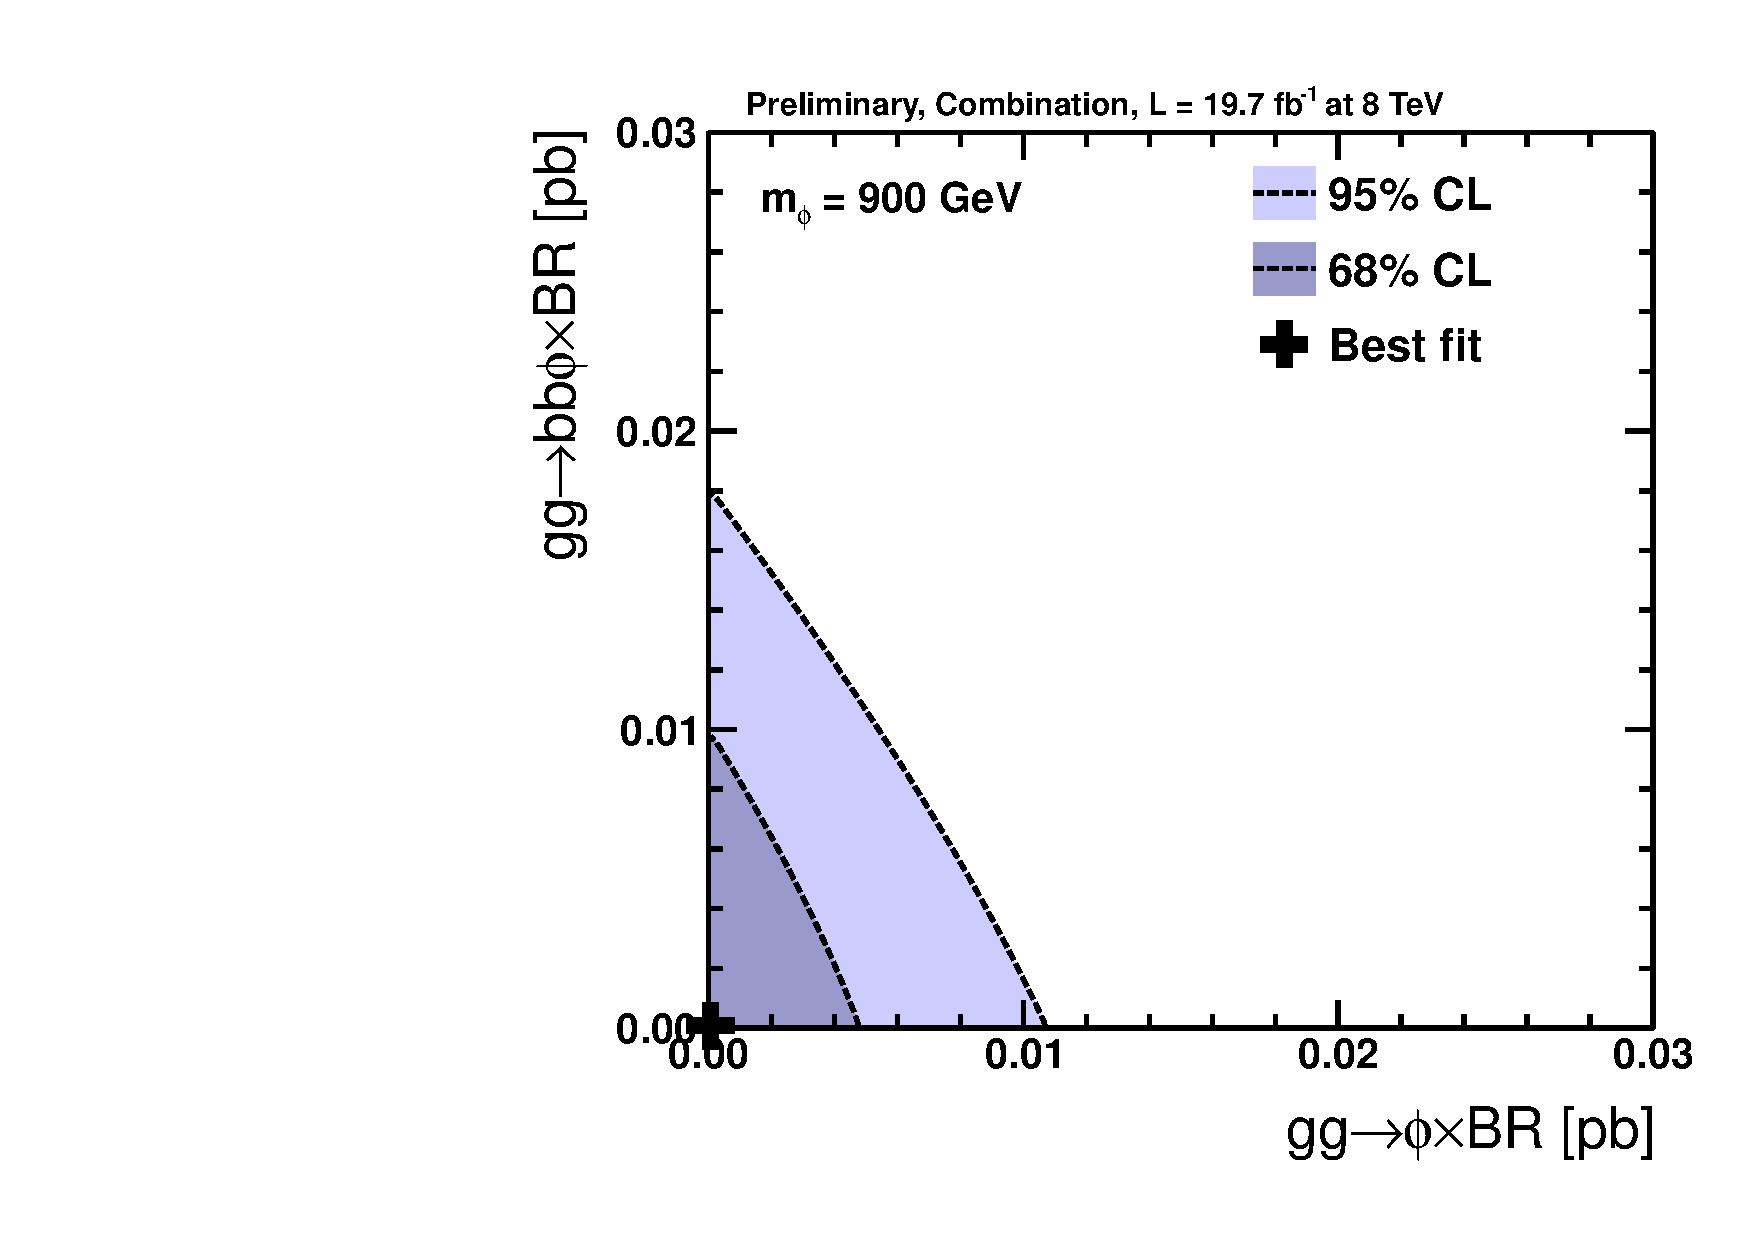
\includegraphics[width=0.45\textwidth]{MSSM/PLOTS/cmb-ggH-bbH-scan-GGH-BBH-900.pdf}
 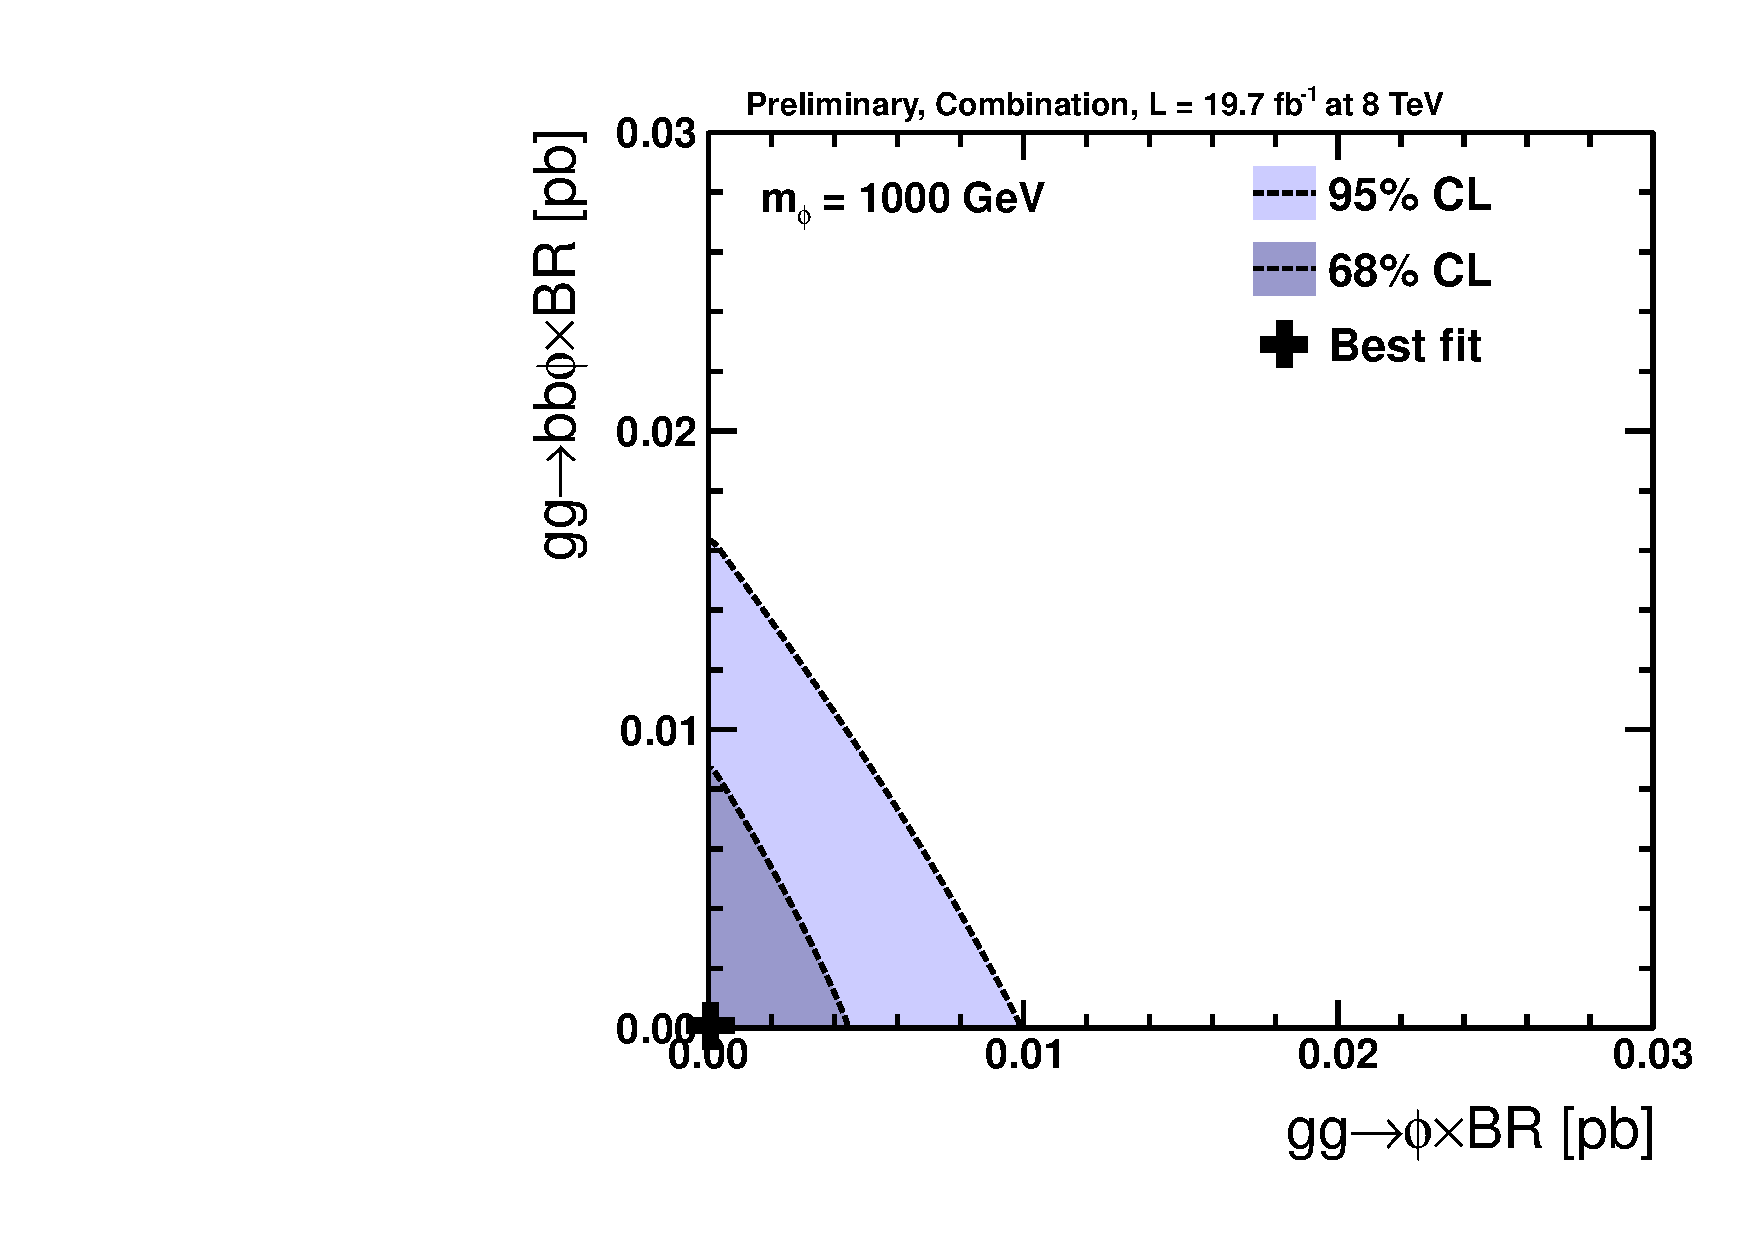
\includegraphics[width=0.45\textwidth]{MSSM/PLOTS/cmb-ggH-bbH-scan-GGH-BBH-1000.pdf}
 \caption{Likelihood contours of $\sigma\times$ BR(gg$\Phi$) and $\sigma\times$ BR(bb$\Phi$) at 8 TeV center-of-mass energy for different Higgs boson masses}
  \label{fig:contour4}\end{center}\end{figure*}

\clearpage

\section{Summary}
A search for neutral Higgs bosons decaying to tau pairs has been performed using events recorded by the CMS experiment at the LHC
in 2011 and 2012 at a center-of-mass energy of 7 TeV and 8 TeV respectively. The dataset corresponds to an integrated luminosity of 24.6 fb$^{-1}$, with 4.9 fb$^{-1}$ at 7 TeV and 19.7 fb$^{-1}$ at 8 TeV. Five different $\Pgt\Pgt$ final states are studied: $\Pe\Pgt_{h}, \Pgm\Pgt_{h}, \Pe\Pgm$, $\Pgm\Pgm$ and $\Pgt_{h}\Pgt_{h}$. 
To enhance the sensitivity to neutral Higgs bosons from the minimal supersymmetric extension of the standard model (MSSM), 
events containing zero and and events containing one b-tagged jet are analyzed in separate categories.
No excess is observed in the tau-pair invariant-mass spectrum. Exclusion limits in the MSSM parameter space have been obtained for the $m_h^{\rm max}$ scenario. This search extends previous results to larger values of $M_A$ and excluded values of tan$\beta$ as low as $4.2$ at $M_A=140$~$\GeV$. 
Model independent upper limits on the Higgs boson production cross section times branching fraction for gluon-gluon fusion and b-associated production are also given.





